\chapter{Design and evaluation of the Paper Prototype}


This chapter describes the design and the evaluation of the paper prototype. The design was done on paper and with the knowledge of usability issues in mind. The existing approaches of eco-feedback applications have been evaluated in the section~\ref{sec:approaches}. Especially the design principles were the basis for the hand-sketched drafts. The evaluation was done in a paper prototype session with the users found with the questionnaire. The workshops were held not only done to test usability but first and foremost to answer 

\textbf{RQ 4: Do the characteristics of user groups correlate with the users' preferred type of visualization?}

The mobile application of ASCR will be investigated in particular and will be the basis for the paper prototypes.

As described before in \ref{section:paperprototyping} we follow the Step-by-Step guide of Arnowitz et al. \cite{arnowitz2010effective} to create a Paper Prototype. The first task of the Step-by-Step guide is to define the tasks in a scenario narration.

\textbf{Scenario narration} \quad The main goal of the mobile application for which the paper prototype is sketched is to give eco-feedback. This feedback shall primarily focus on the consumption of electricity, water and heating and the emission of carbon-dioxide. So the history consumption rate of these data shall be available to look into. A comparison of the consumption during different time intervals shall also be possible. This comparison can be drawn to one's own consumption but also to a comparable household, to an average consumption rate of the neighbours, the city or the European Union. On a dashboard the current measured values, the consumption of the day and some current settings shall be shown. The management of the home automation system shall also be available via the app. Tips for saving money by saving energy shall also be given. Energy saving-tips shall be tailored to the characteristics of a user type. Especially for Hedonists the menu item "Project" will be interesting. Here projects are listed, which show possible further home automation items that can help at energy saving. A user can read frequently asked questions in the FAQ section.

\section{Design of Paper Prototype}
Having in mind the above mentioned tasks we designed multiple versions of the paper prototypes that resulted from several runs through the Step-by-Step guide for the creation of a paper prototype of Arnowitz et al. \cite{arnowitz2010effective}. The outcomes of these process are described below. For better readability we describe the user interfaces followed by the results of the paper prototyping sessions.

\section{Menu navigation}

We developed a navigation drawer and adapted it to the requirements of each user type, as shown in Figure ~\ref{fig:drawer}. The sorting of the menu items was adapted to the main motivation why a user uses the app.

\textbf{Improvements} \quad The test user from the Optimizer and Indifferent user section stated that a drag and drop function to resort the items would be a nice-to-have feature. One Optimizer suggested to use a different colour for each menu item to make it visually more appealing. Also the use of icons was highly recommended.

\begin{figure}[h]
	\centering
	\begin{subfigure}[b]{0.24\columnwidth}
		\centering
		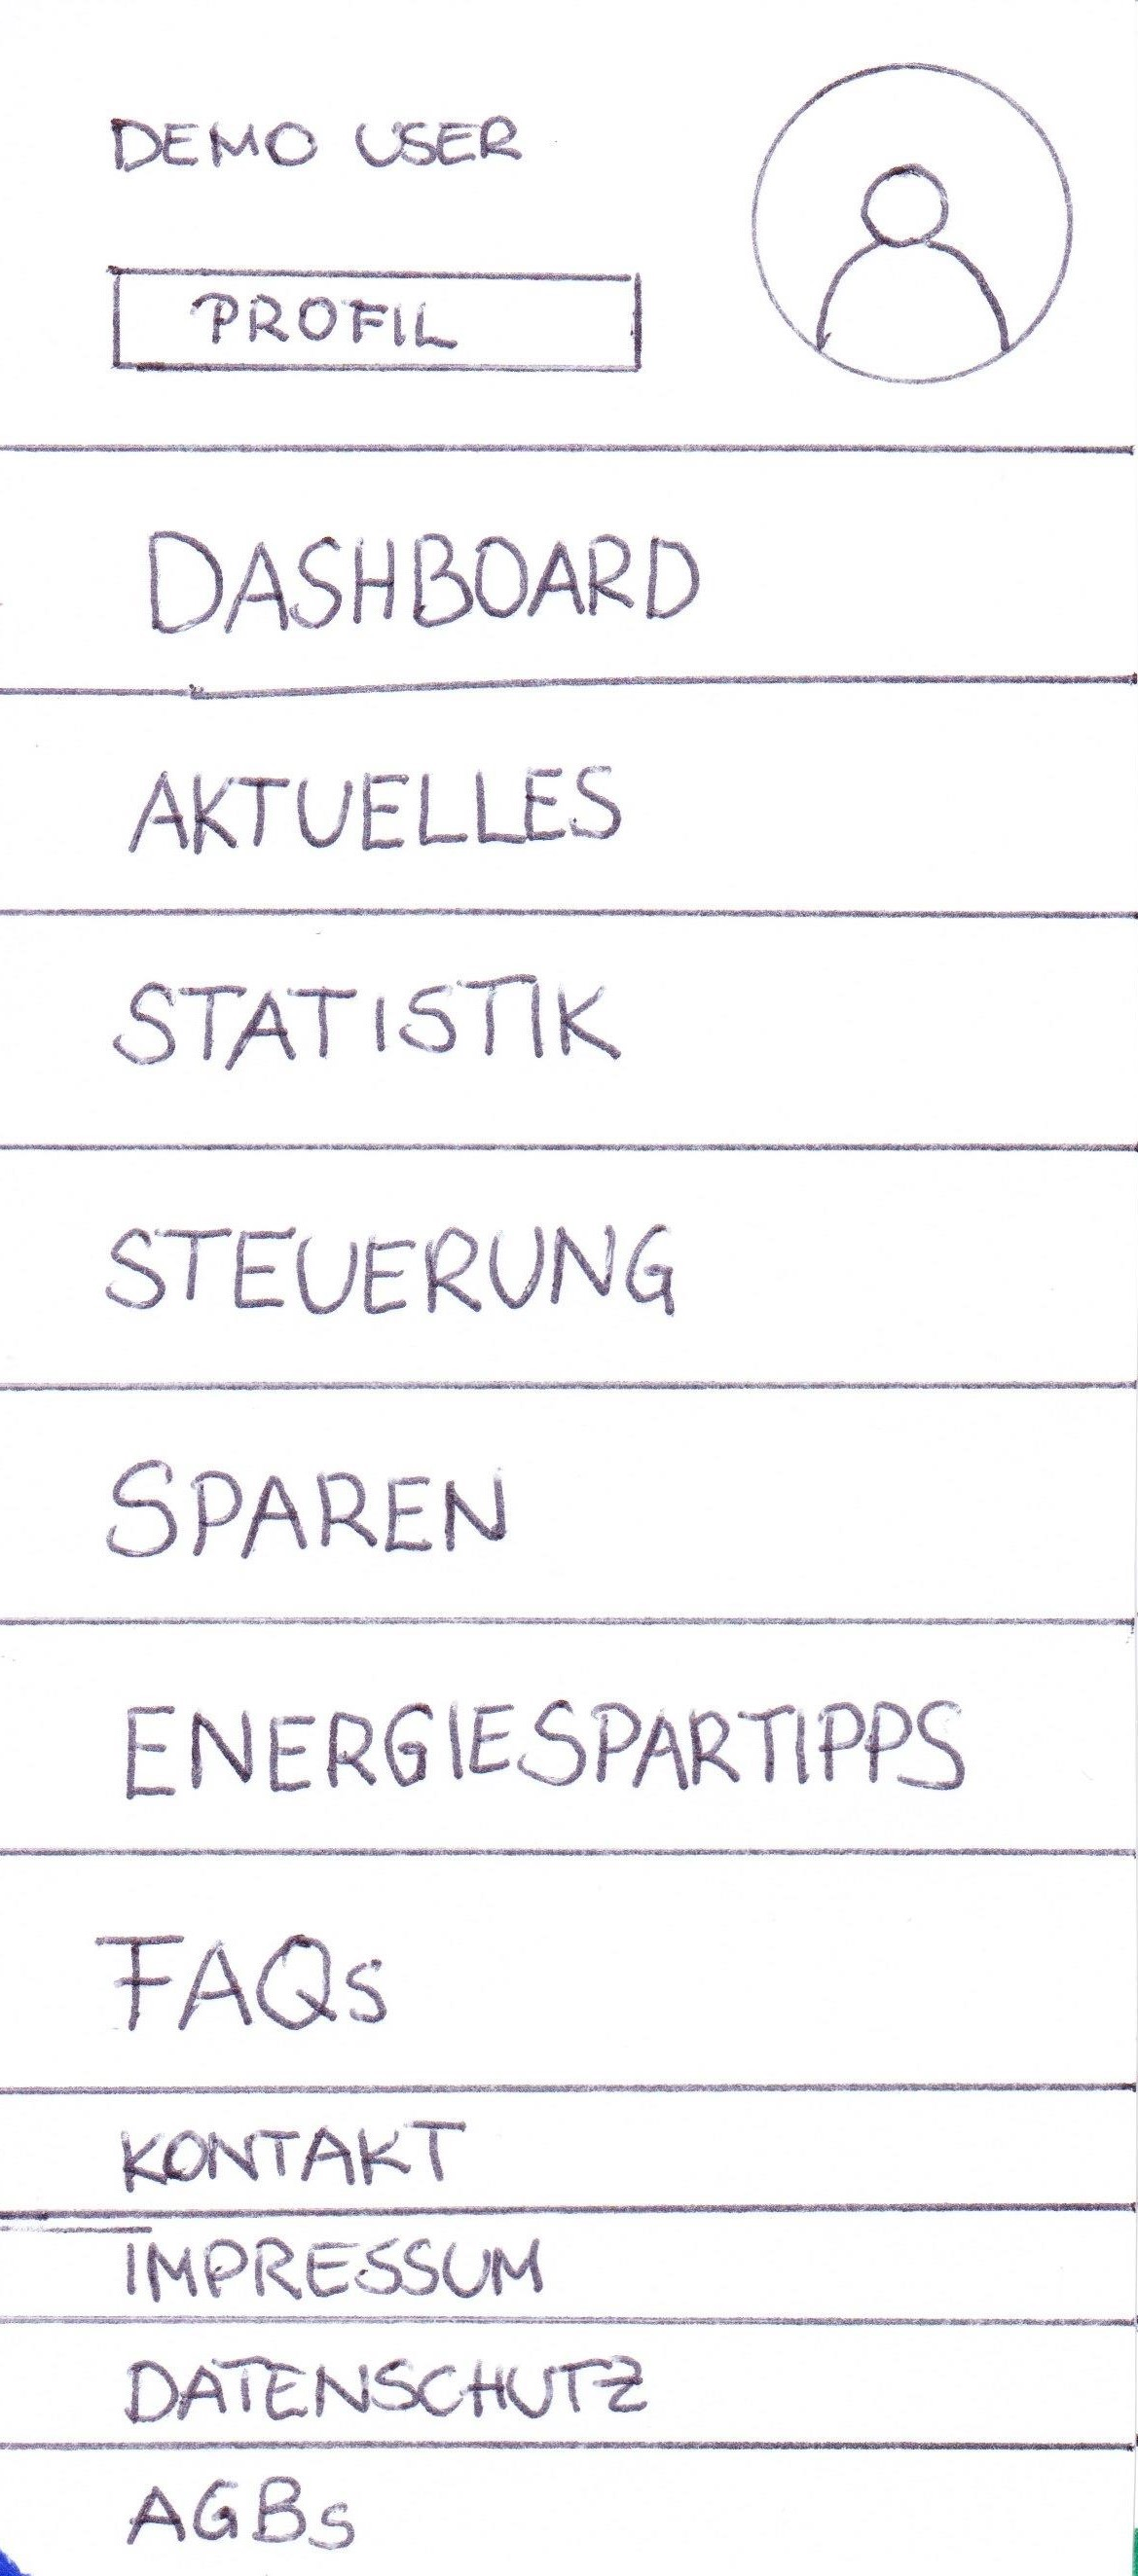
\includegraphics[width=\textwidth]{screens/drawer_1}
		\subcaption{Professional}
		\label{fig:drawer:professional}
	\end{subfigure}
	\begin{subfigure}[b]{0.24\columnwidth}
		\centering
		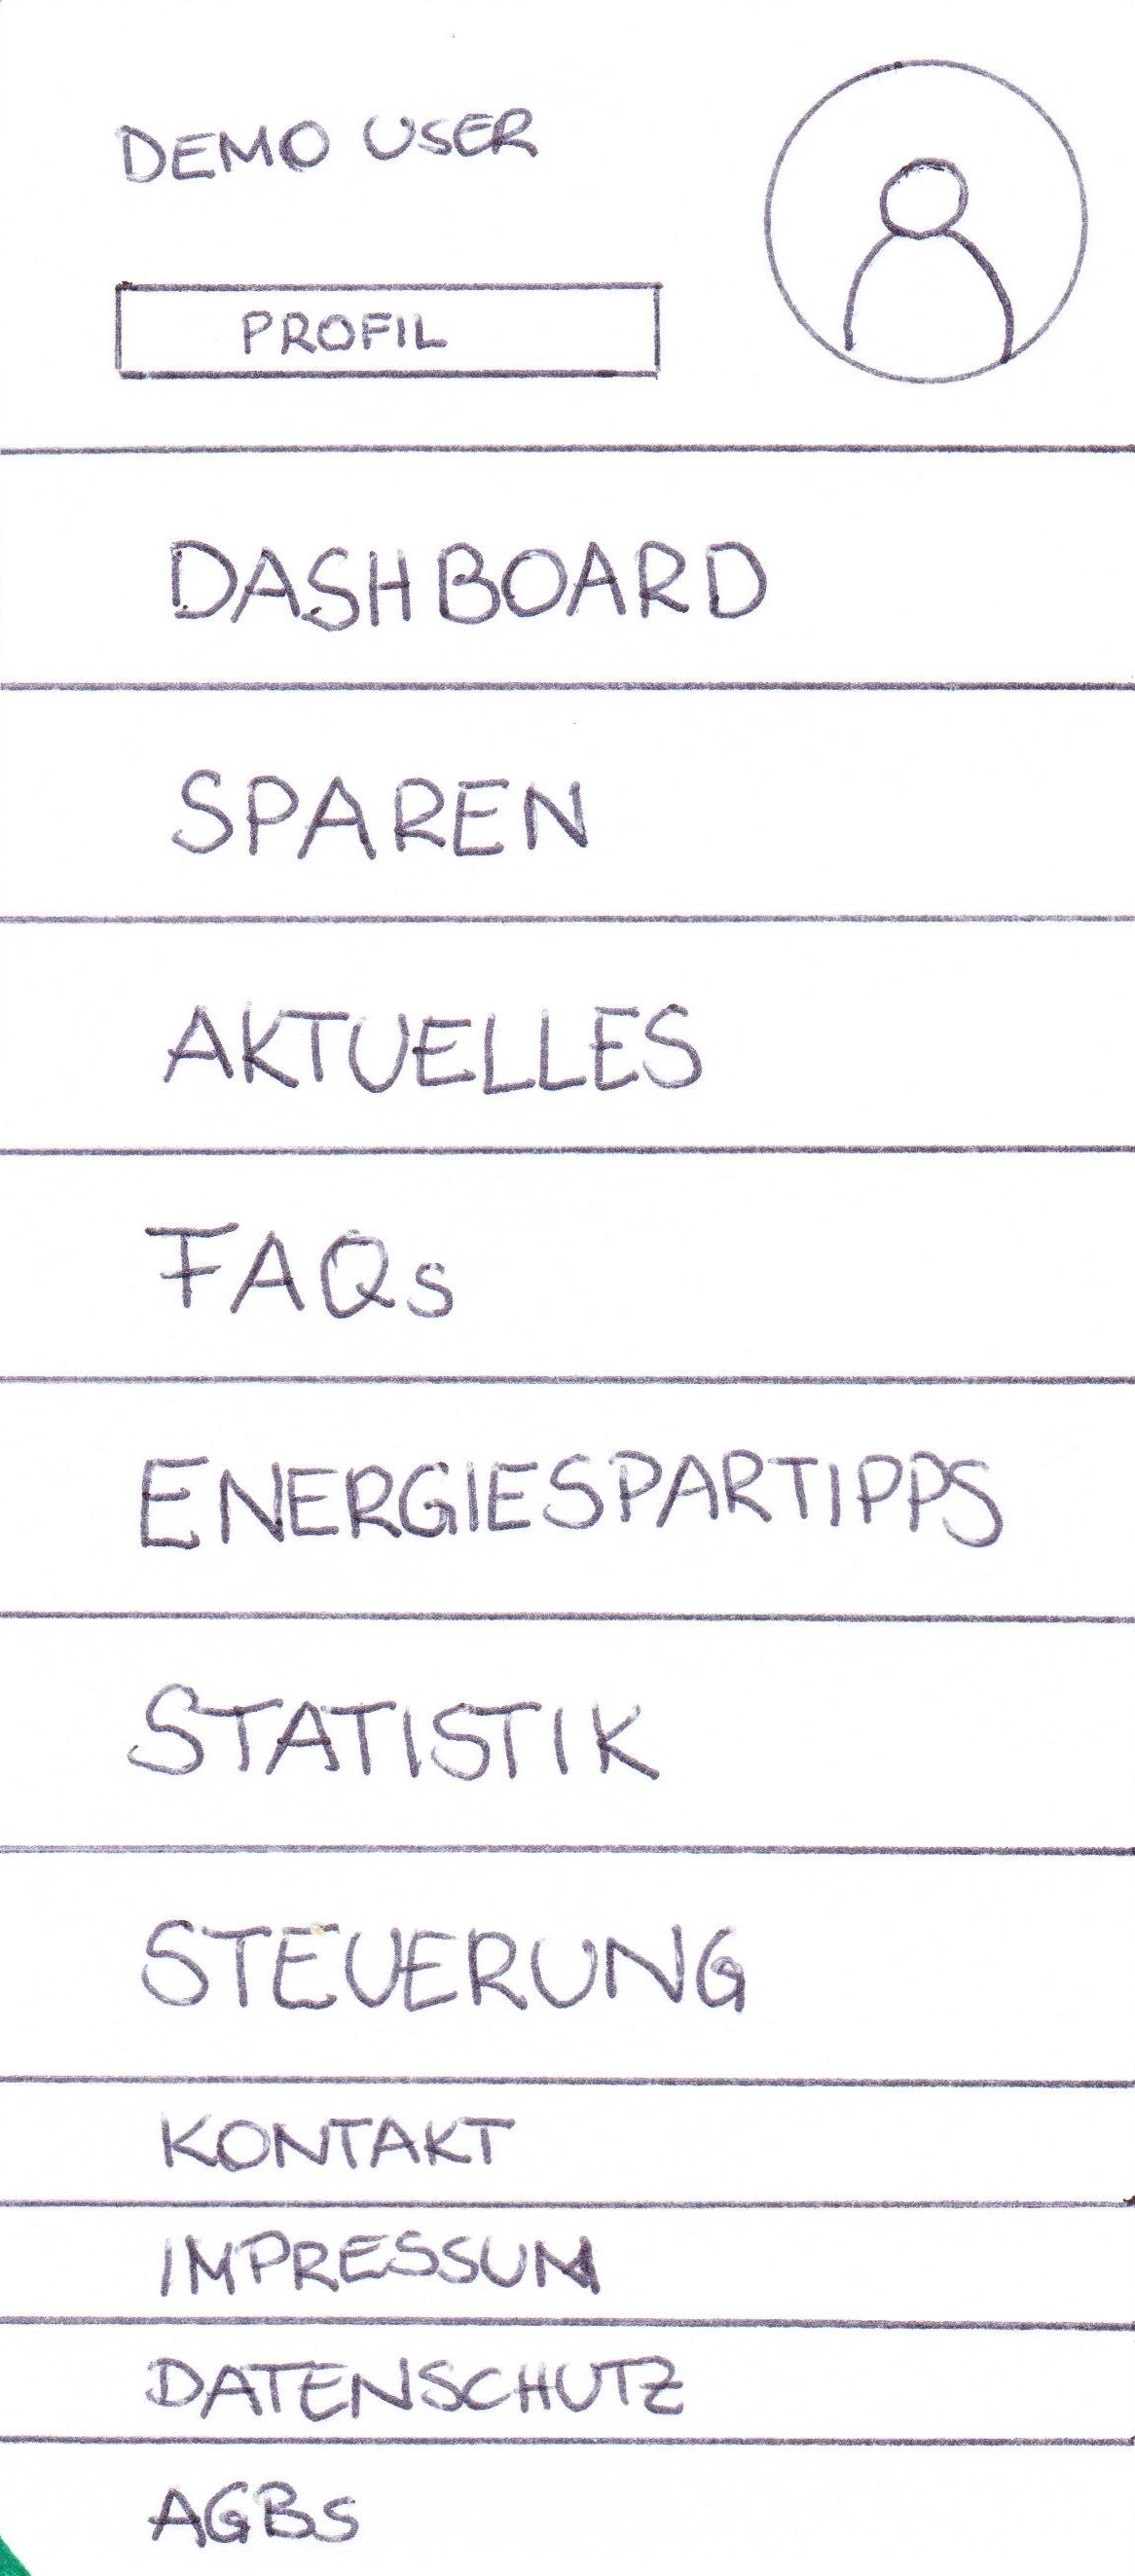
\includegraphics[width=\textwidth]{screens/drawer_2}
		\subcaption{Optimizer}
		\label{fig:drawer:optimizer}
	\end{subfigure}
	\begin{subfigure}[b]{0.24\columnwidth}
		\centering
		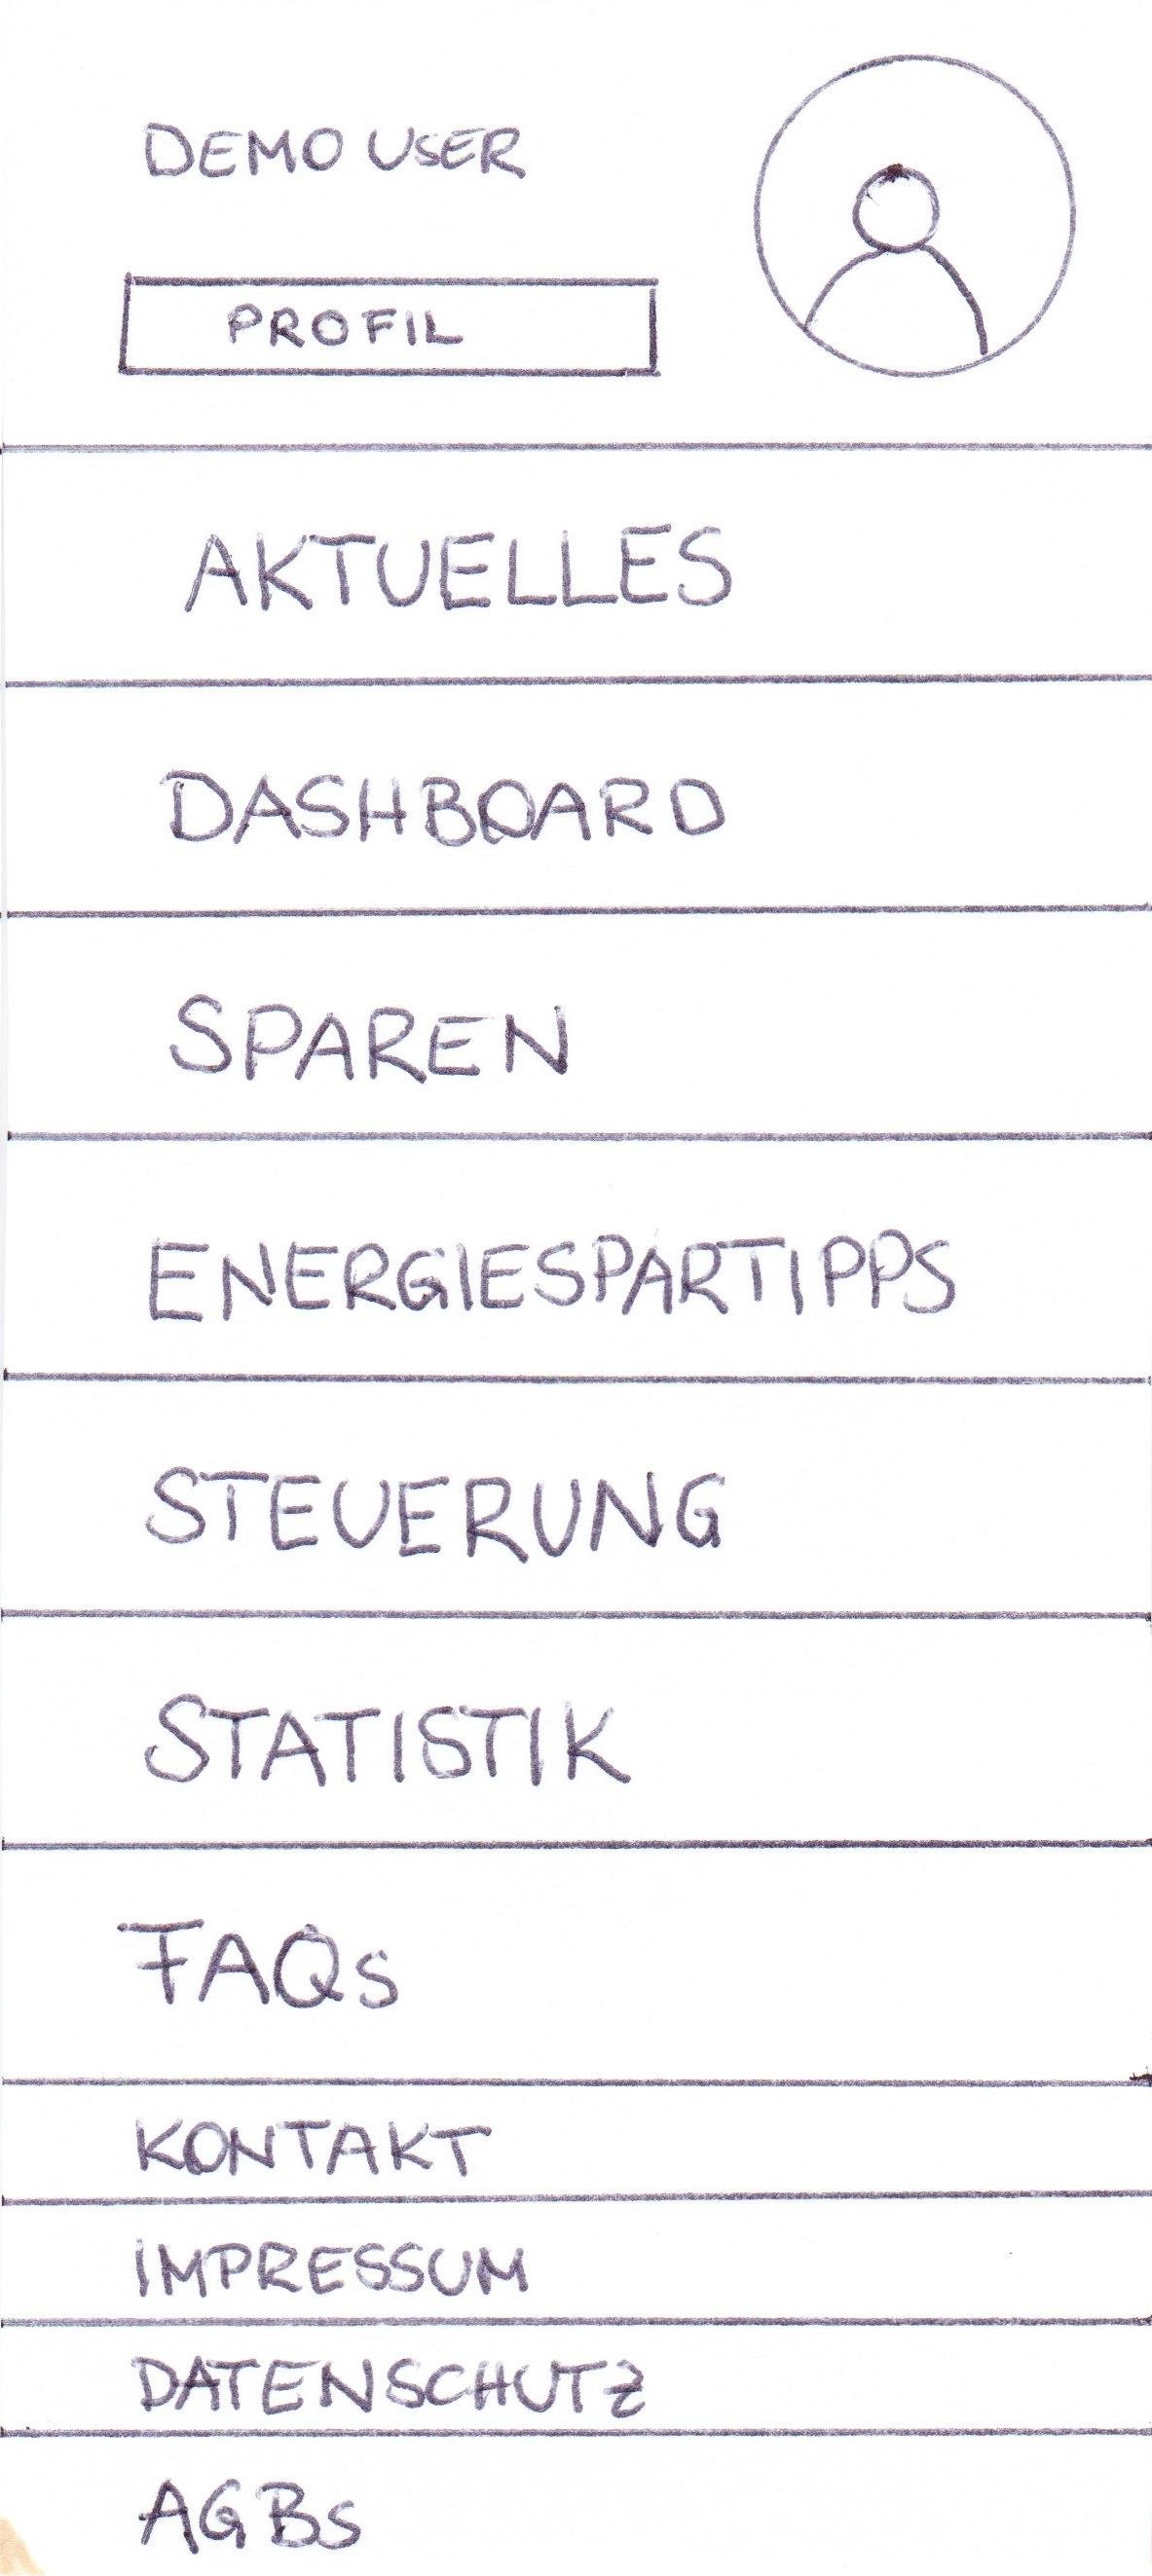
\includegraphics[width=\textwidth]{screens/drawer_3}
		\subcaption{Indifferent}
		\label{fig:drawer:indifferent}
	\end{subfigure}
	\begin{subfigure}[b]{0.24\columnwidth}
		\centering
		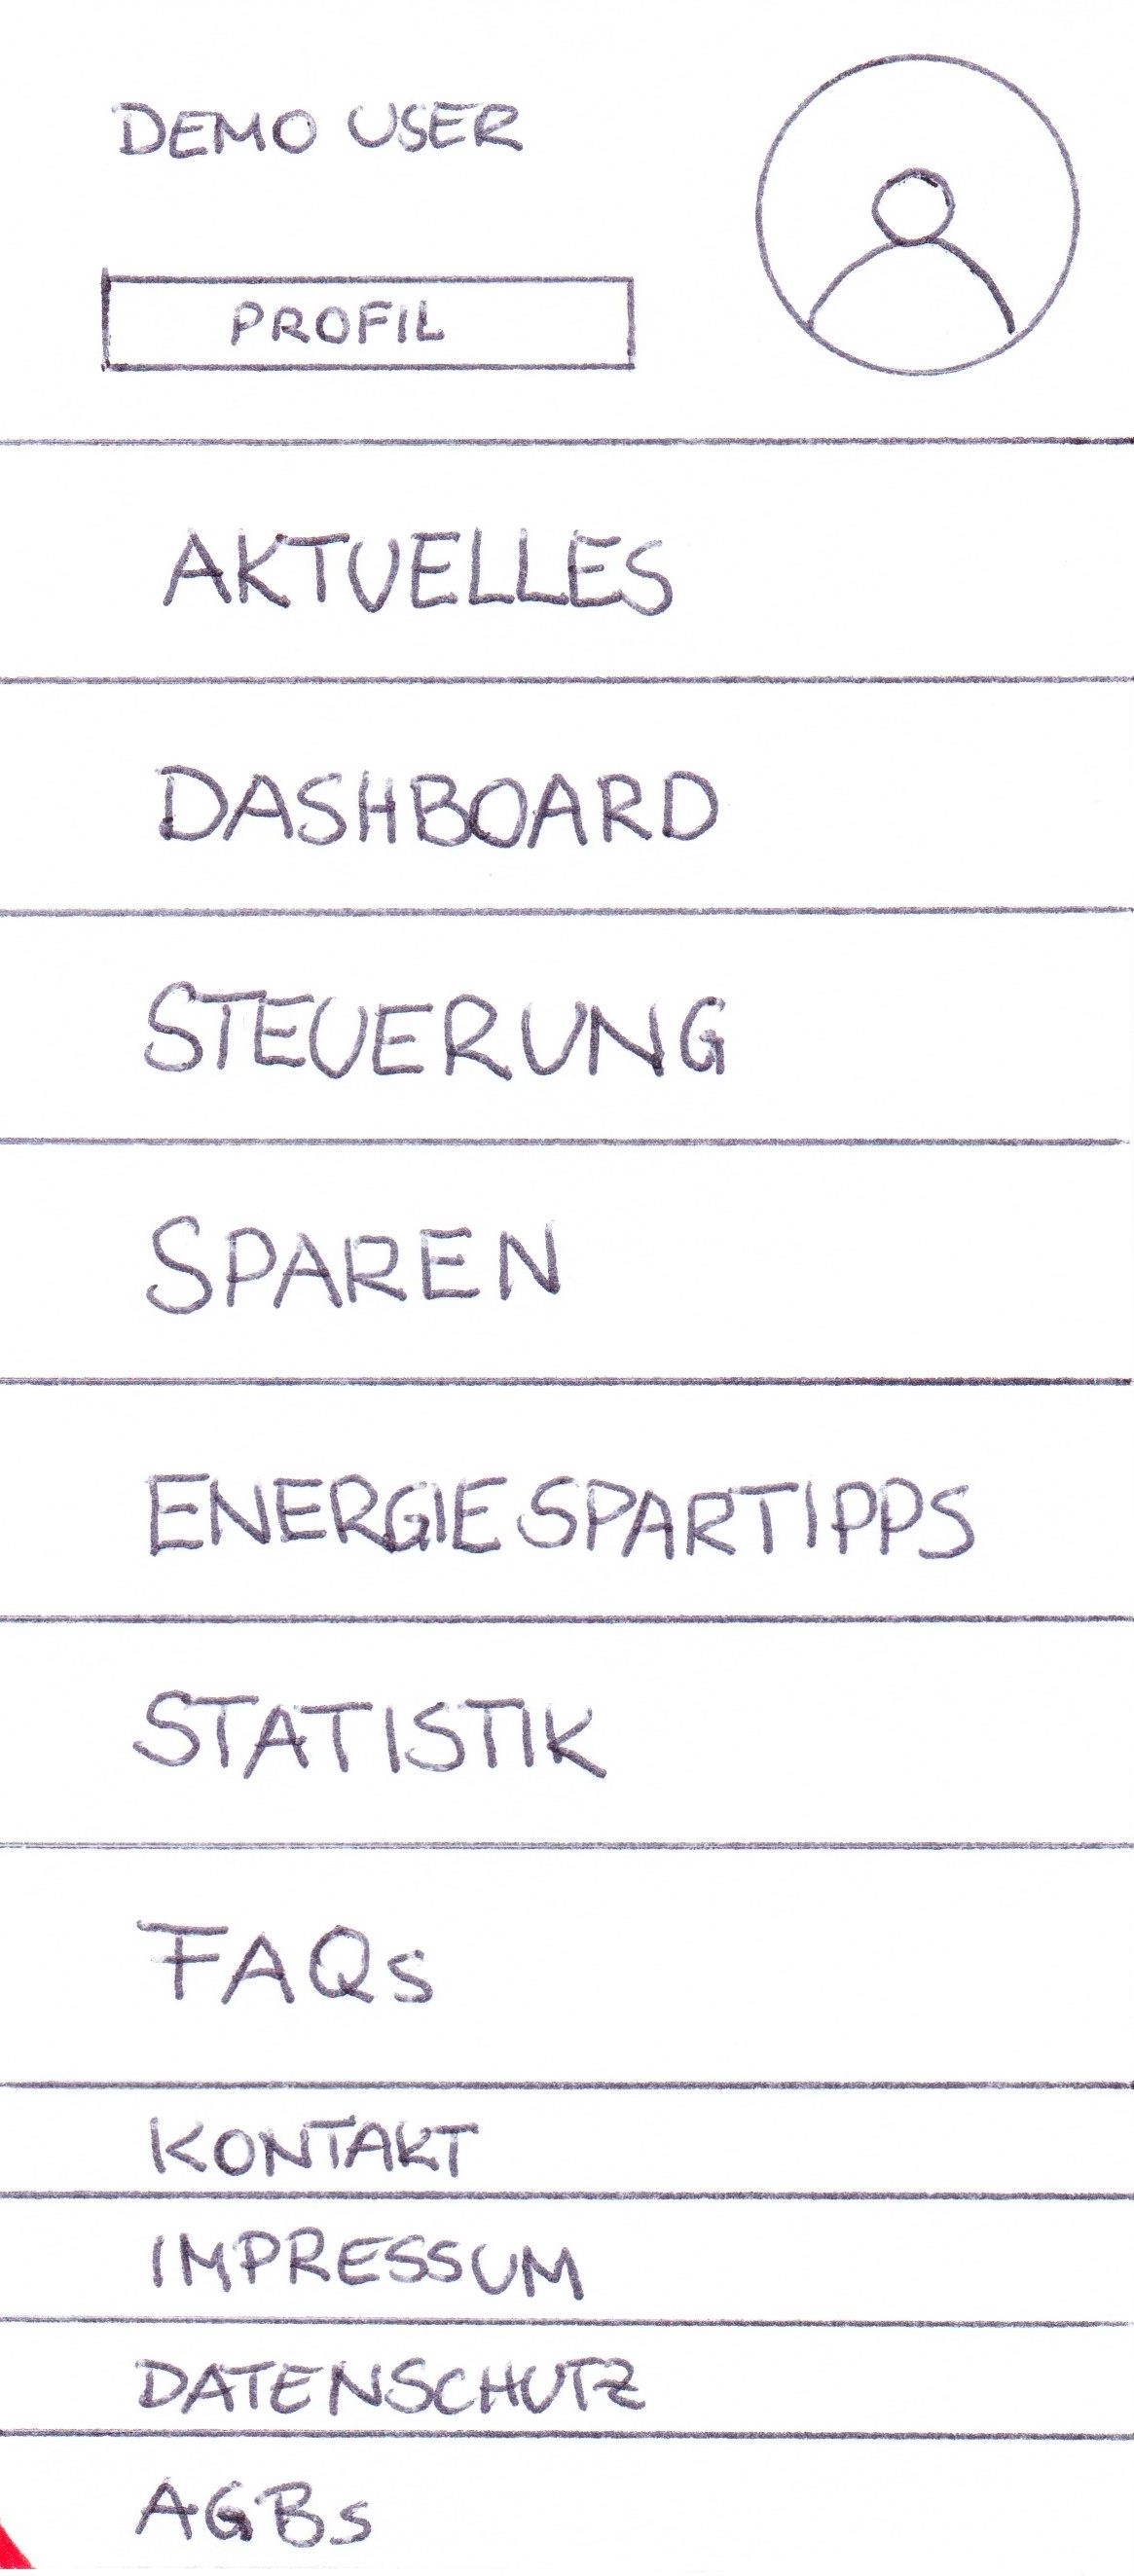
\includegraphics[width=\textwidth]{screens/drawer_4}
		\subcaption{Hedonist}
		\label{fig:drawer:hedonist}
	\end{subfigure}
	\caption{Proposed screens for the navigation drawer}
	\label{fig:drawer} % \label has to be placed AFTER \caption (or \subcaption) to produce correct cross-references.
\end{figure}


\subsection*{Guideline 1: Adapt navigation drawer to requirements of user type}

 Sort the items of the navigation drawer according to the motivation of a user type. An effect would be that a user can quickly interact with the app as the preferred items are on top. The sorting reduces the time a user has to search for his/her primary task. However, the different sorting can be irritating when a user compares the app to a user who is a different type of energy user and therefore has another look of the app.
 
\textbf{Evidence} \quad The paper prototype session with the professionals has shown that Professionals primarily use the app for monitoring their consumption rate, therefore the Dashboard is the first menu item. The main motivation for Optimizer is to save money with the app. Indifferents primarily use the app because it makes fun which means that their main motivation is supported by the gamification approach. Hedonists' are especially motivated to use the app, when their drive for programming projects is picked up. The gamification approach and the projects are shown in the first menu item, for that reason the Dashboard is on second place for Hedonists and Indifferents. The following user stories were tested in the paper prototype session with the according user types and were proven to appropriate:
\begin{itemize}
	\item As a Professional I primarily use the app to monitor my consumption rate.
	\item As an Optimizer I primarily use the app to save money.
	\item As an Indifferent I primarily use the app for fun.
	\item As a Hedonist I primarily use the app to manage my home automation gadgets.
\end{itemize}


\section{Measurements}

The dashboard was based on the one from the ASCR application. As visible in~\ref{fig:dashboard}, the main difference is the use of kWh for Professionals and Hedonists and the use of Euro for Optimizer and Indifferents. Especially the scale of the air humidity was stated as appealing from the test users.

\textbf{Improvements} \quad One critic from a Professional was, that the screen misses, how the quality of the air can be improved. Grouping the measured values to one side and the values that can be controlled to the other side was also suggested by a Professional. The Optimizer again wished for more colours and symbols. A similar scale for CO2 as for the air humidity was mentioned by the Indifferent segment of test users. An extra pop up window for the adjustable values was desired from the Hedonist test user.

\begin{figure}[h]
	\centering
	\begin{subfigure}[b]{0.24\columnwidth}
		\centering
		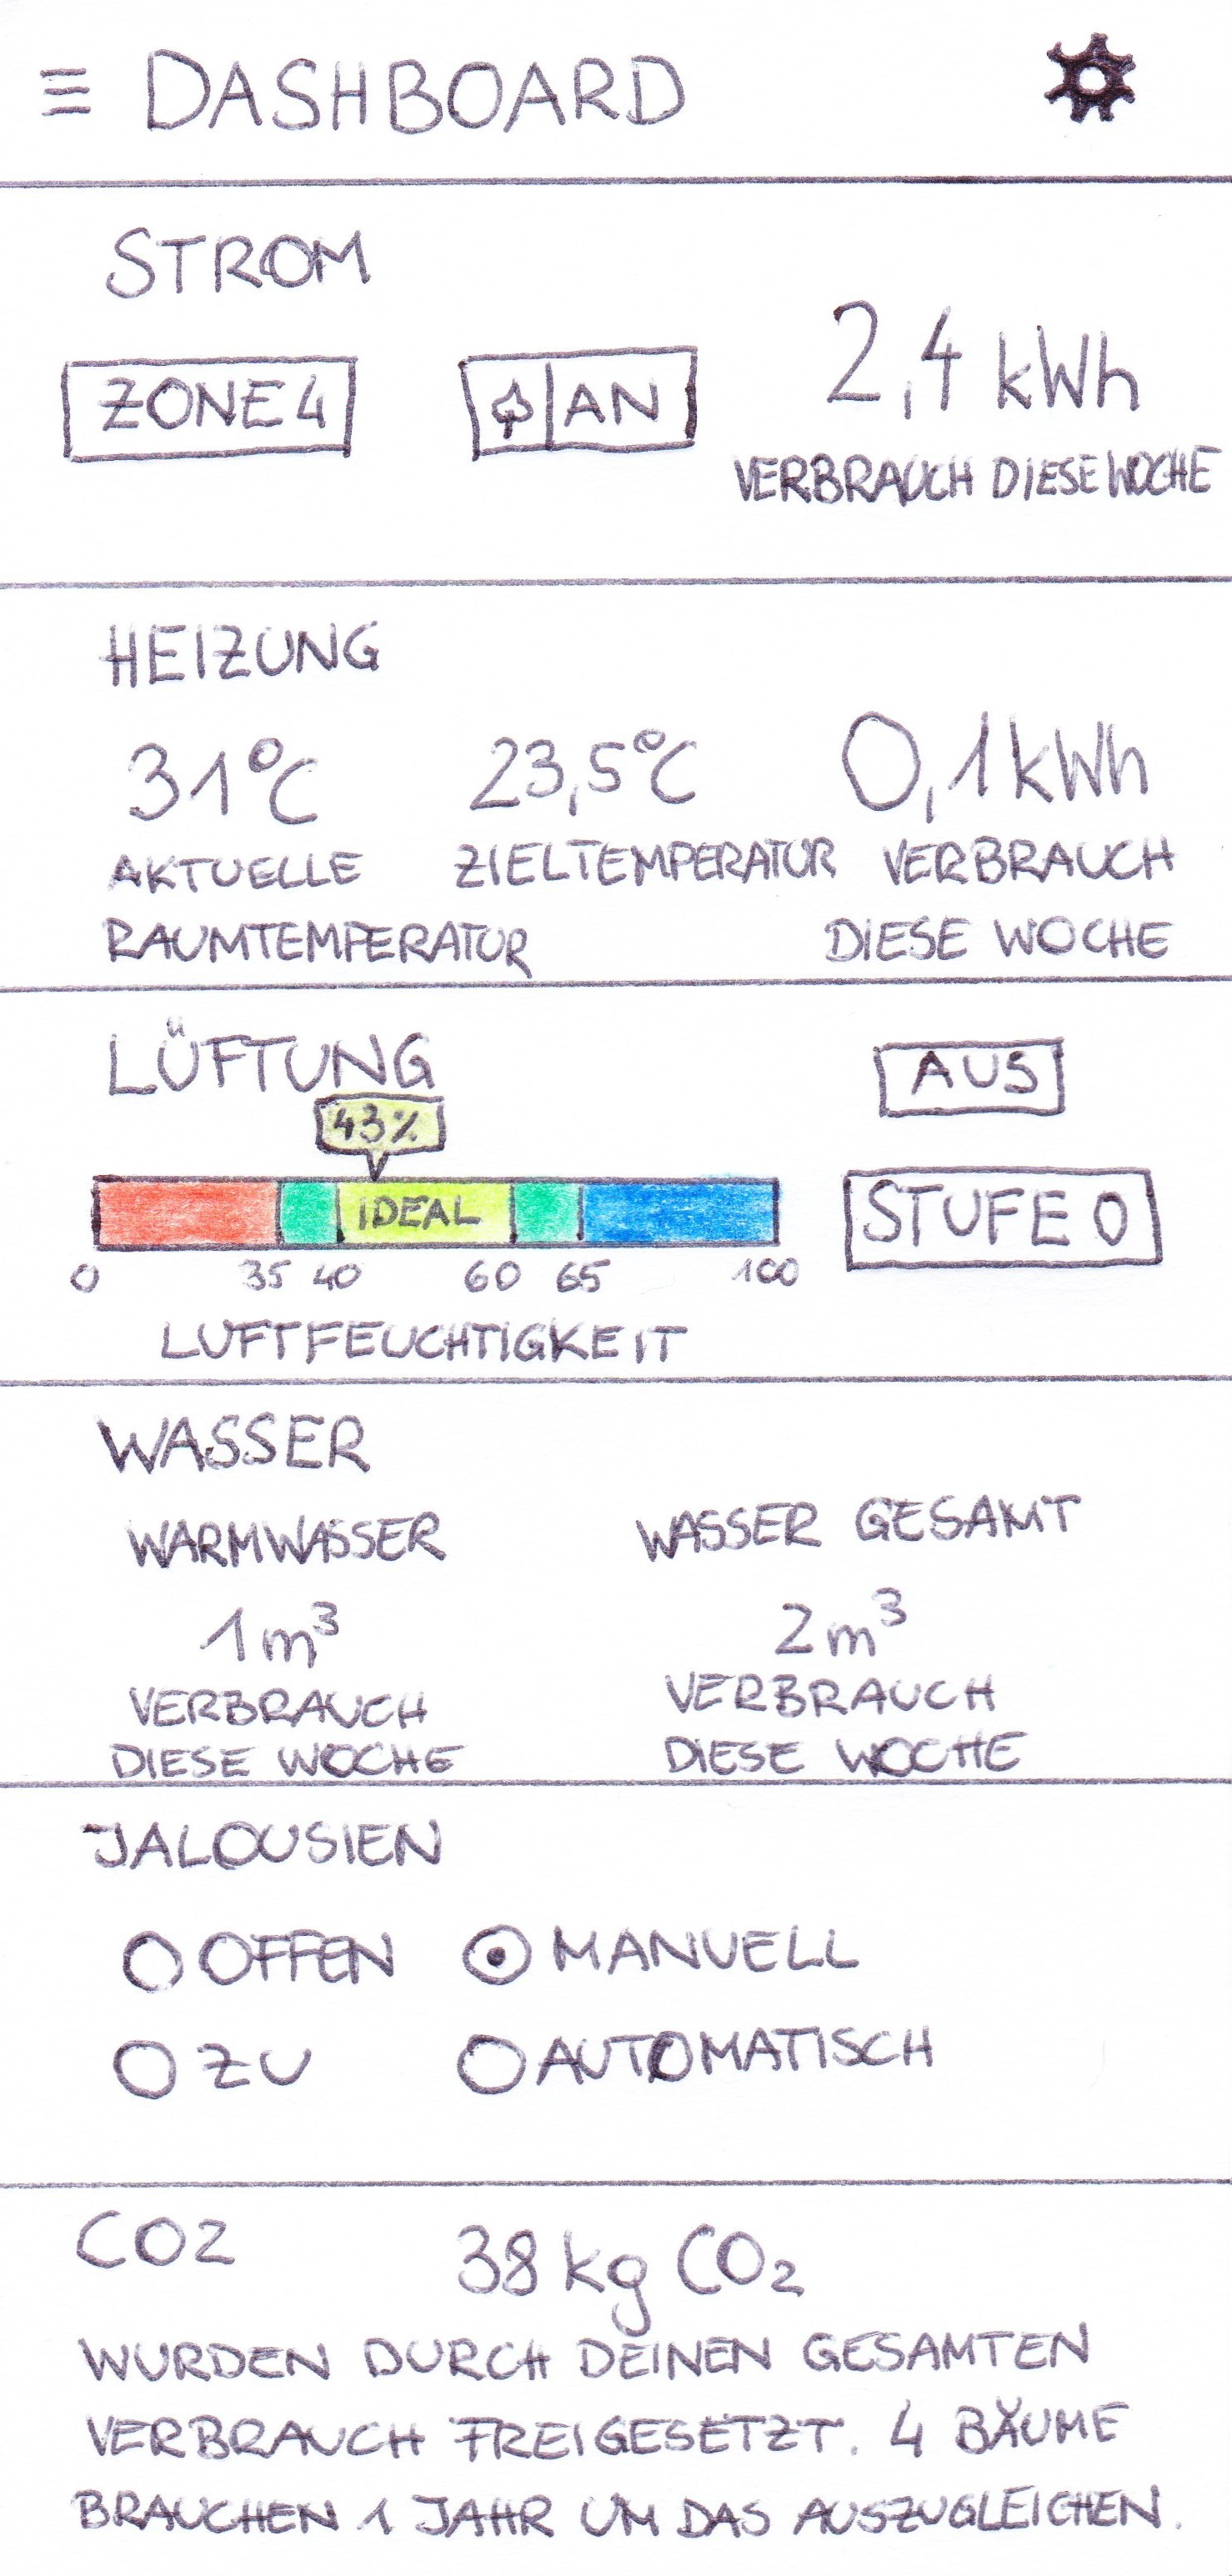
\includegraphics[width=\textwidth]{screens/dashboard_14}
		\subcaption{Professional and Hedonist}
		\label{fig:dasboard:professional}
	\end{subfigure}
	\begin{subfigure}[b]{0.24\columnwidth}
		\centering
		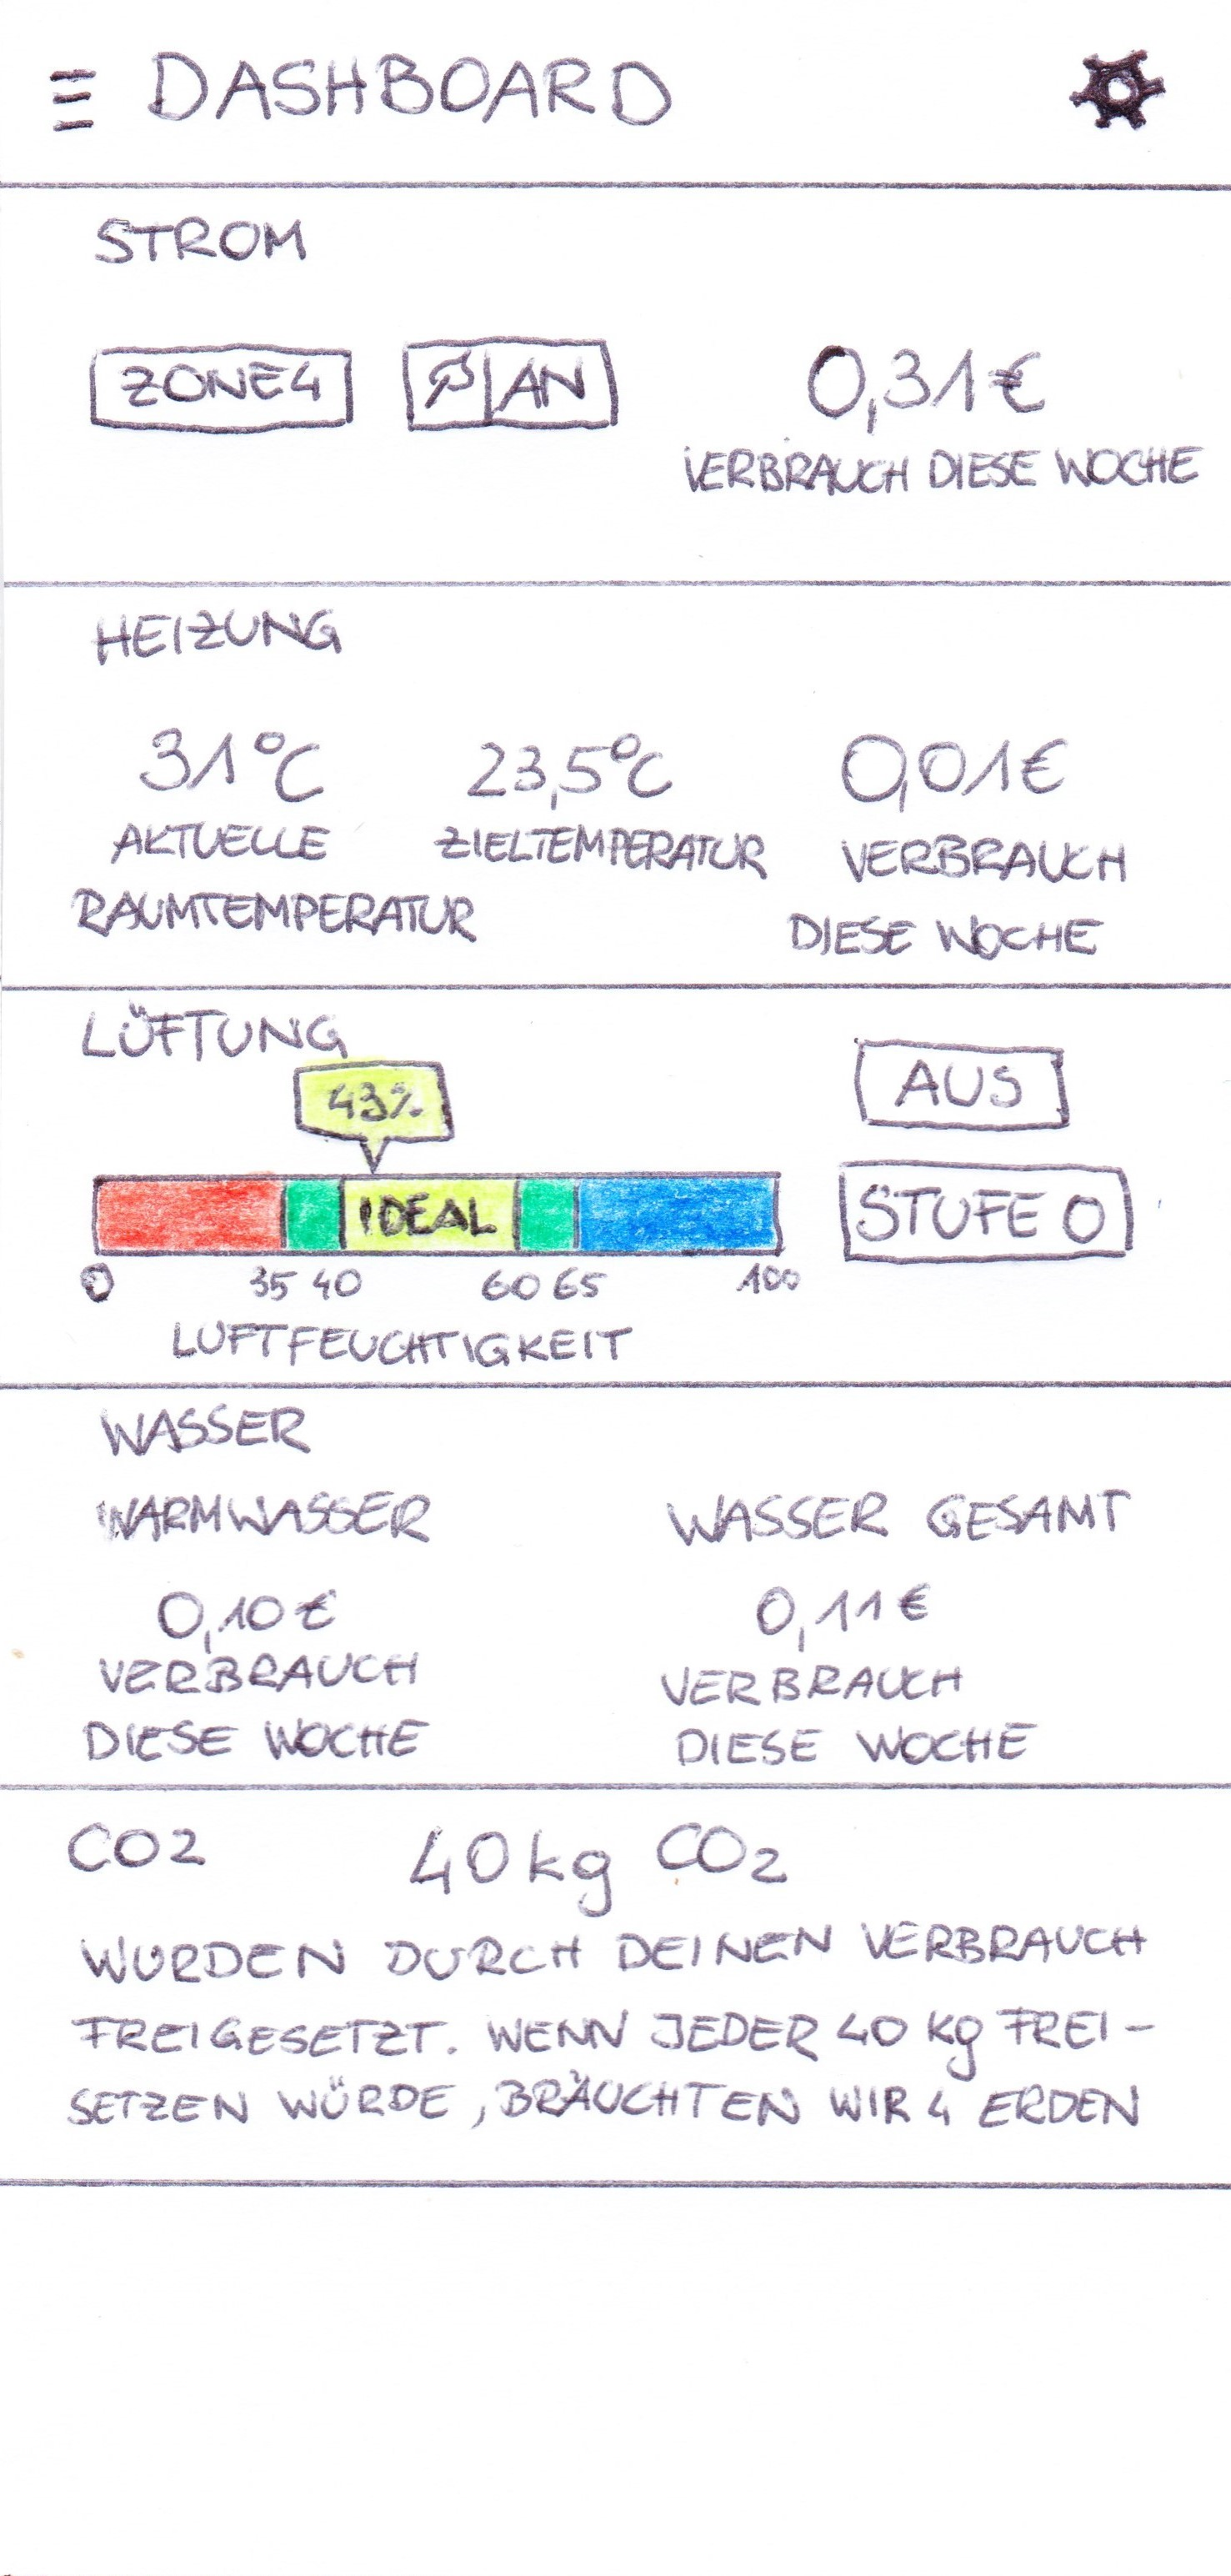
\includegraphics[width=\textwidth]{screens/dashboard_23}
		\subcaption{Optimizer and Indifferent}
		\label{fig:dashboard:optimizer}
	\end{subfigure}
	\caption{Sketches of the dashboard}
	\label{fig:dashboard} % \label has to be placed AFTER \caption (or \subcaption) to produce correct cross-references.
\end{figure}

\subsection*{Guideline 2: Use monetary units for Optimizers and Indifferents and units of energy or consumption for Professionals and Hedonists}

Depending on the user type the measurement unit is changed and the value converted accordingly. The electricity and heating consumption is shown in kWh for Professionals and Hedonists and in Euro for Optimizers and Indifferents. The same counts for consumption of water. Optimizers and Indifferents prefer the measurement unit Euro to cubic meter.

\textbf{Evidence} \quad Tailoring, as mentioned before in ~\nameref{subsec:primaryTask}, is beneficial for persuasion. The tailoring of the measurement unit to the preferences was defined as very beneficial by all user types. It was very clear in all testing sessions that the proposed unit for the particular user group was preferred. The following user stories were shown to be true: 

\begin{itemize}
	\item As a Professional I prefer units of energy or consumption to monetary units.
	\item As an Optimizer I prefer monetary units to units of energy or consumption.
	\item As an Indifferent I prefer monetary units to units of energy or consumption.
	\item As a Hedonist I prefer units of energy or consumption to monetary units.
\end{itemize}

\section{Latest topics}

In the latest topics section, shown in Figure~\ref{fig:aktuelles}, a user can see informations that are daily new. Professionals and Hedonists are given the project item and Optimizer and Indifferents have an overview of the current level and the trophies earned. The latest figures such as "Did you know that...", "Figure of the day...", "Energy-saving tip of the day..." and "Lifehack of the day..." shall motivate the user to use the app daily.

\textbf{Improvements} \quad Some test user mentioned that the information given in the daily news should also be tailored to personal consumption figures. One Professional mentioned that a reminder from time to time for the daily figures would be interesting but at a daily basis it would be annoying. The users of the other segments came to the same conclusion. The Hedonist test user group said that for the project overview only the next to-do would be enough and the bread crumbs from the latest steps are not necessary.

\begin{figure}[h]
	\centering
	\begin{subfigure}[b]{0.24\columnwidth}
		\centering
		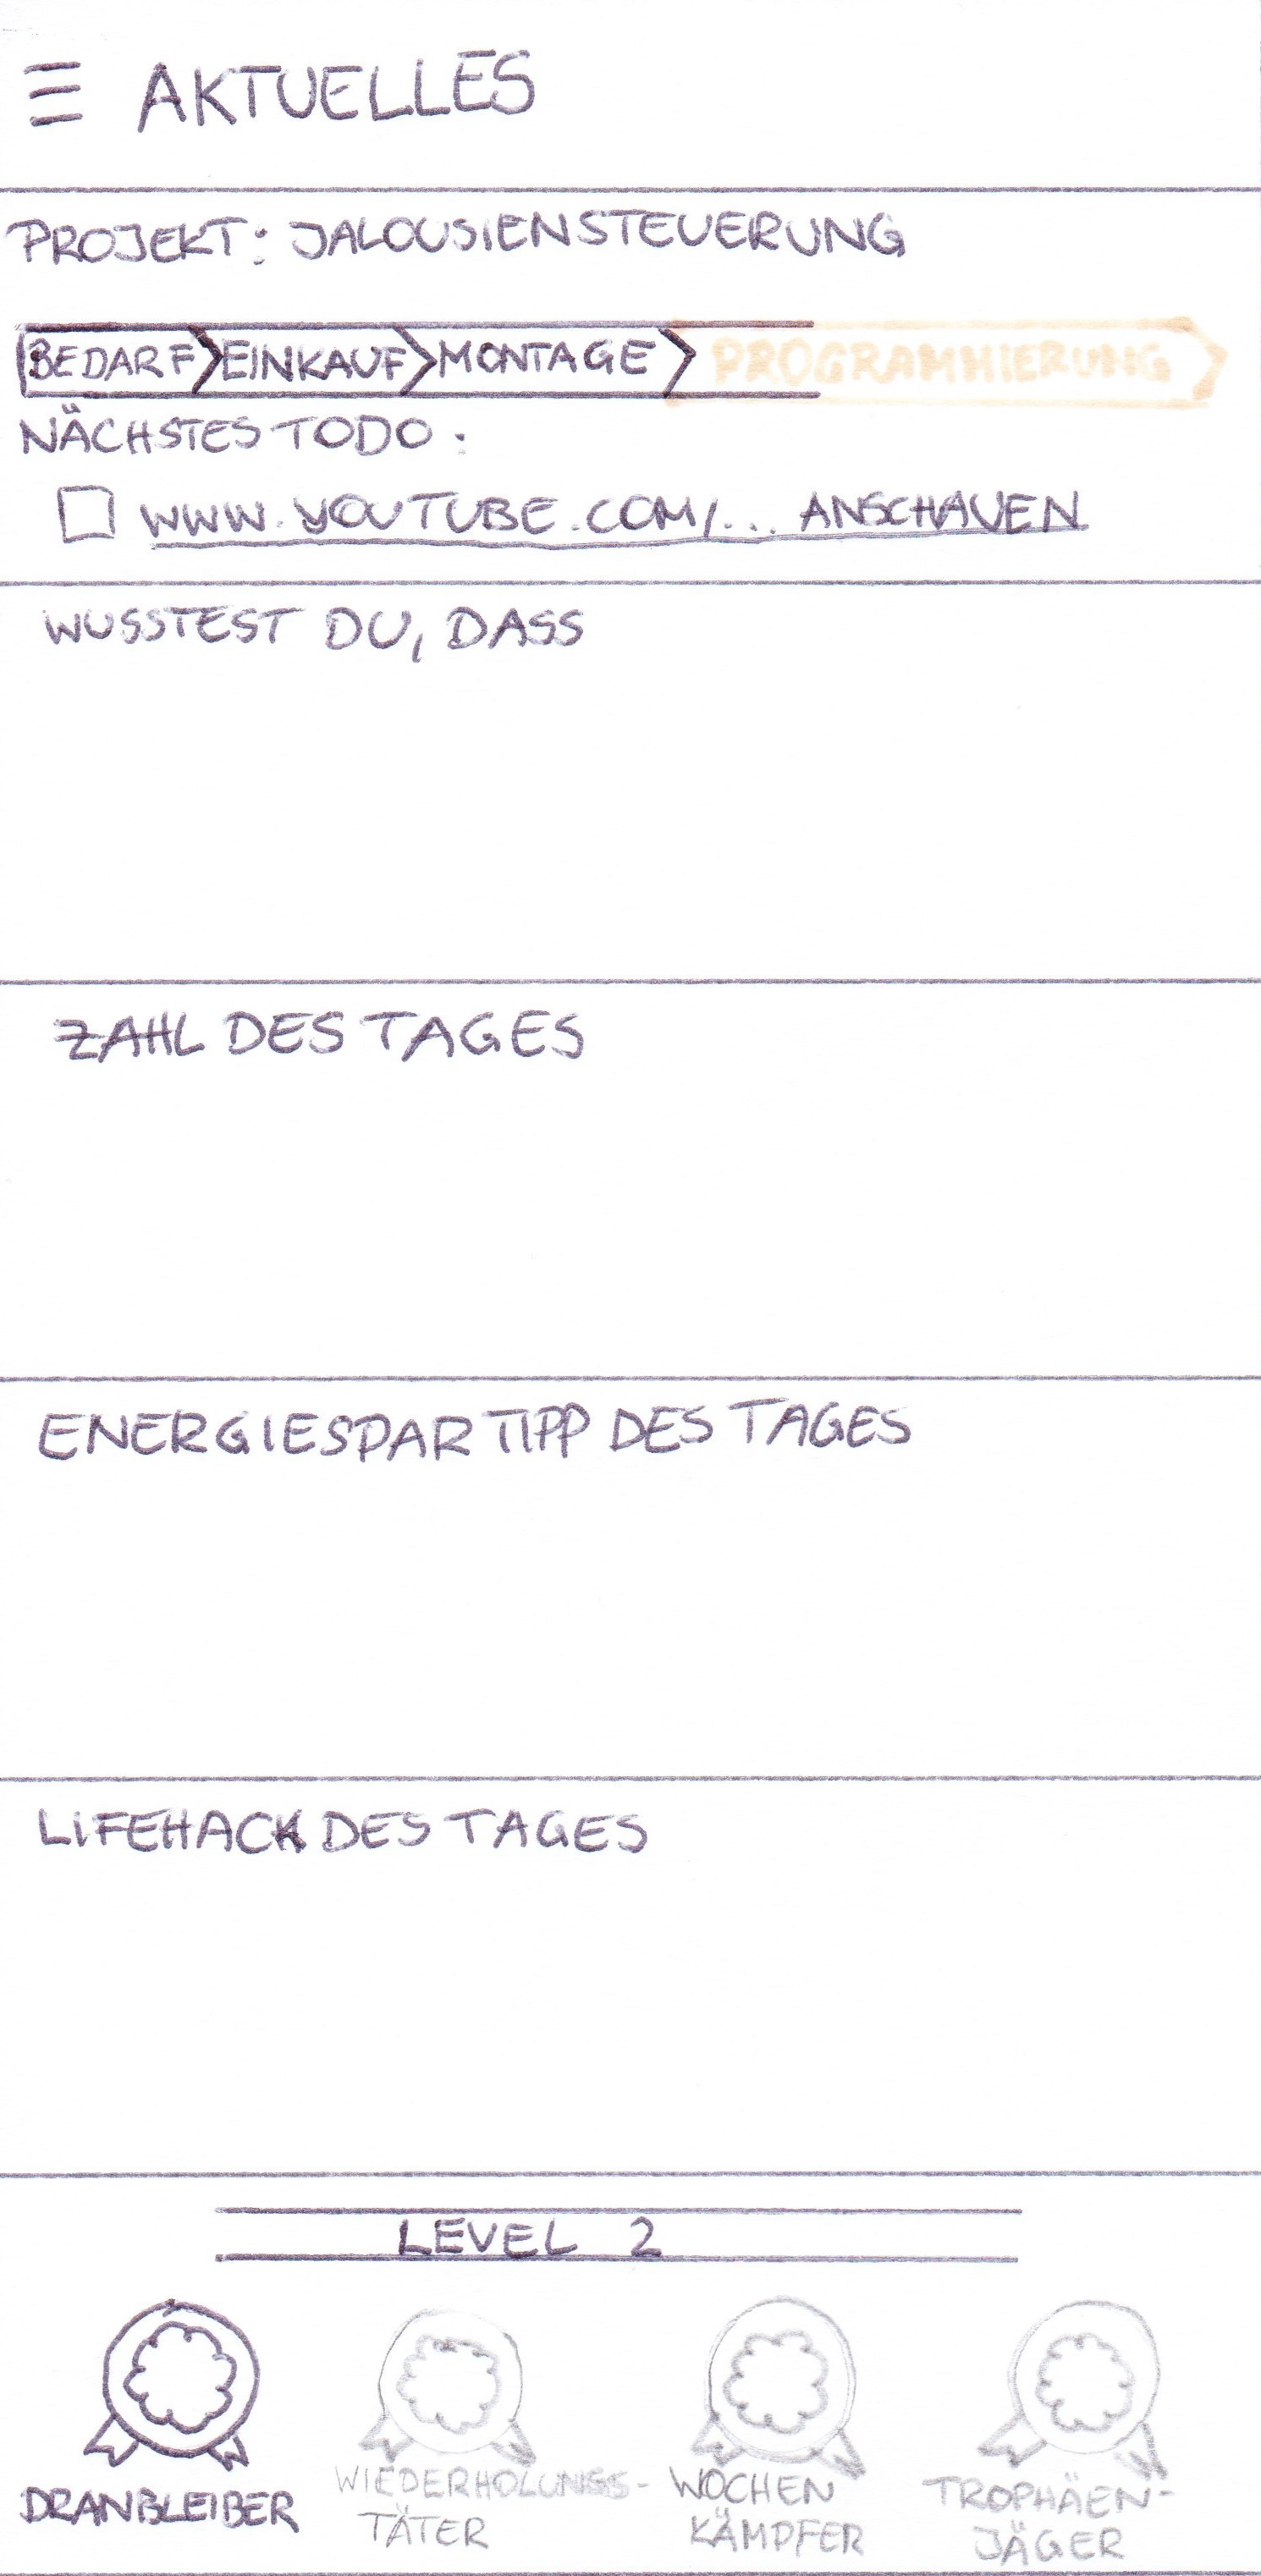
\includegraphics[width=\textwidth]{screens/aktuelles_14}
		\subcaption{Professional and Hedonist}
		\label{fig:aktuelles:professional}
	\end{subfigure}
	\begin{subfigure}[b]{0.24\columnwidth}
		\centering
		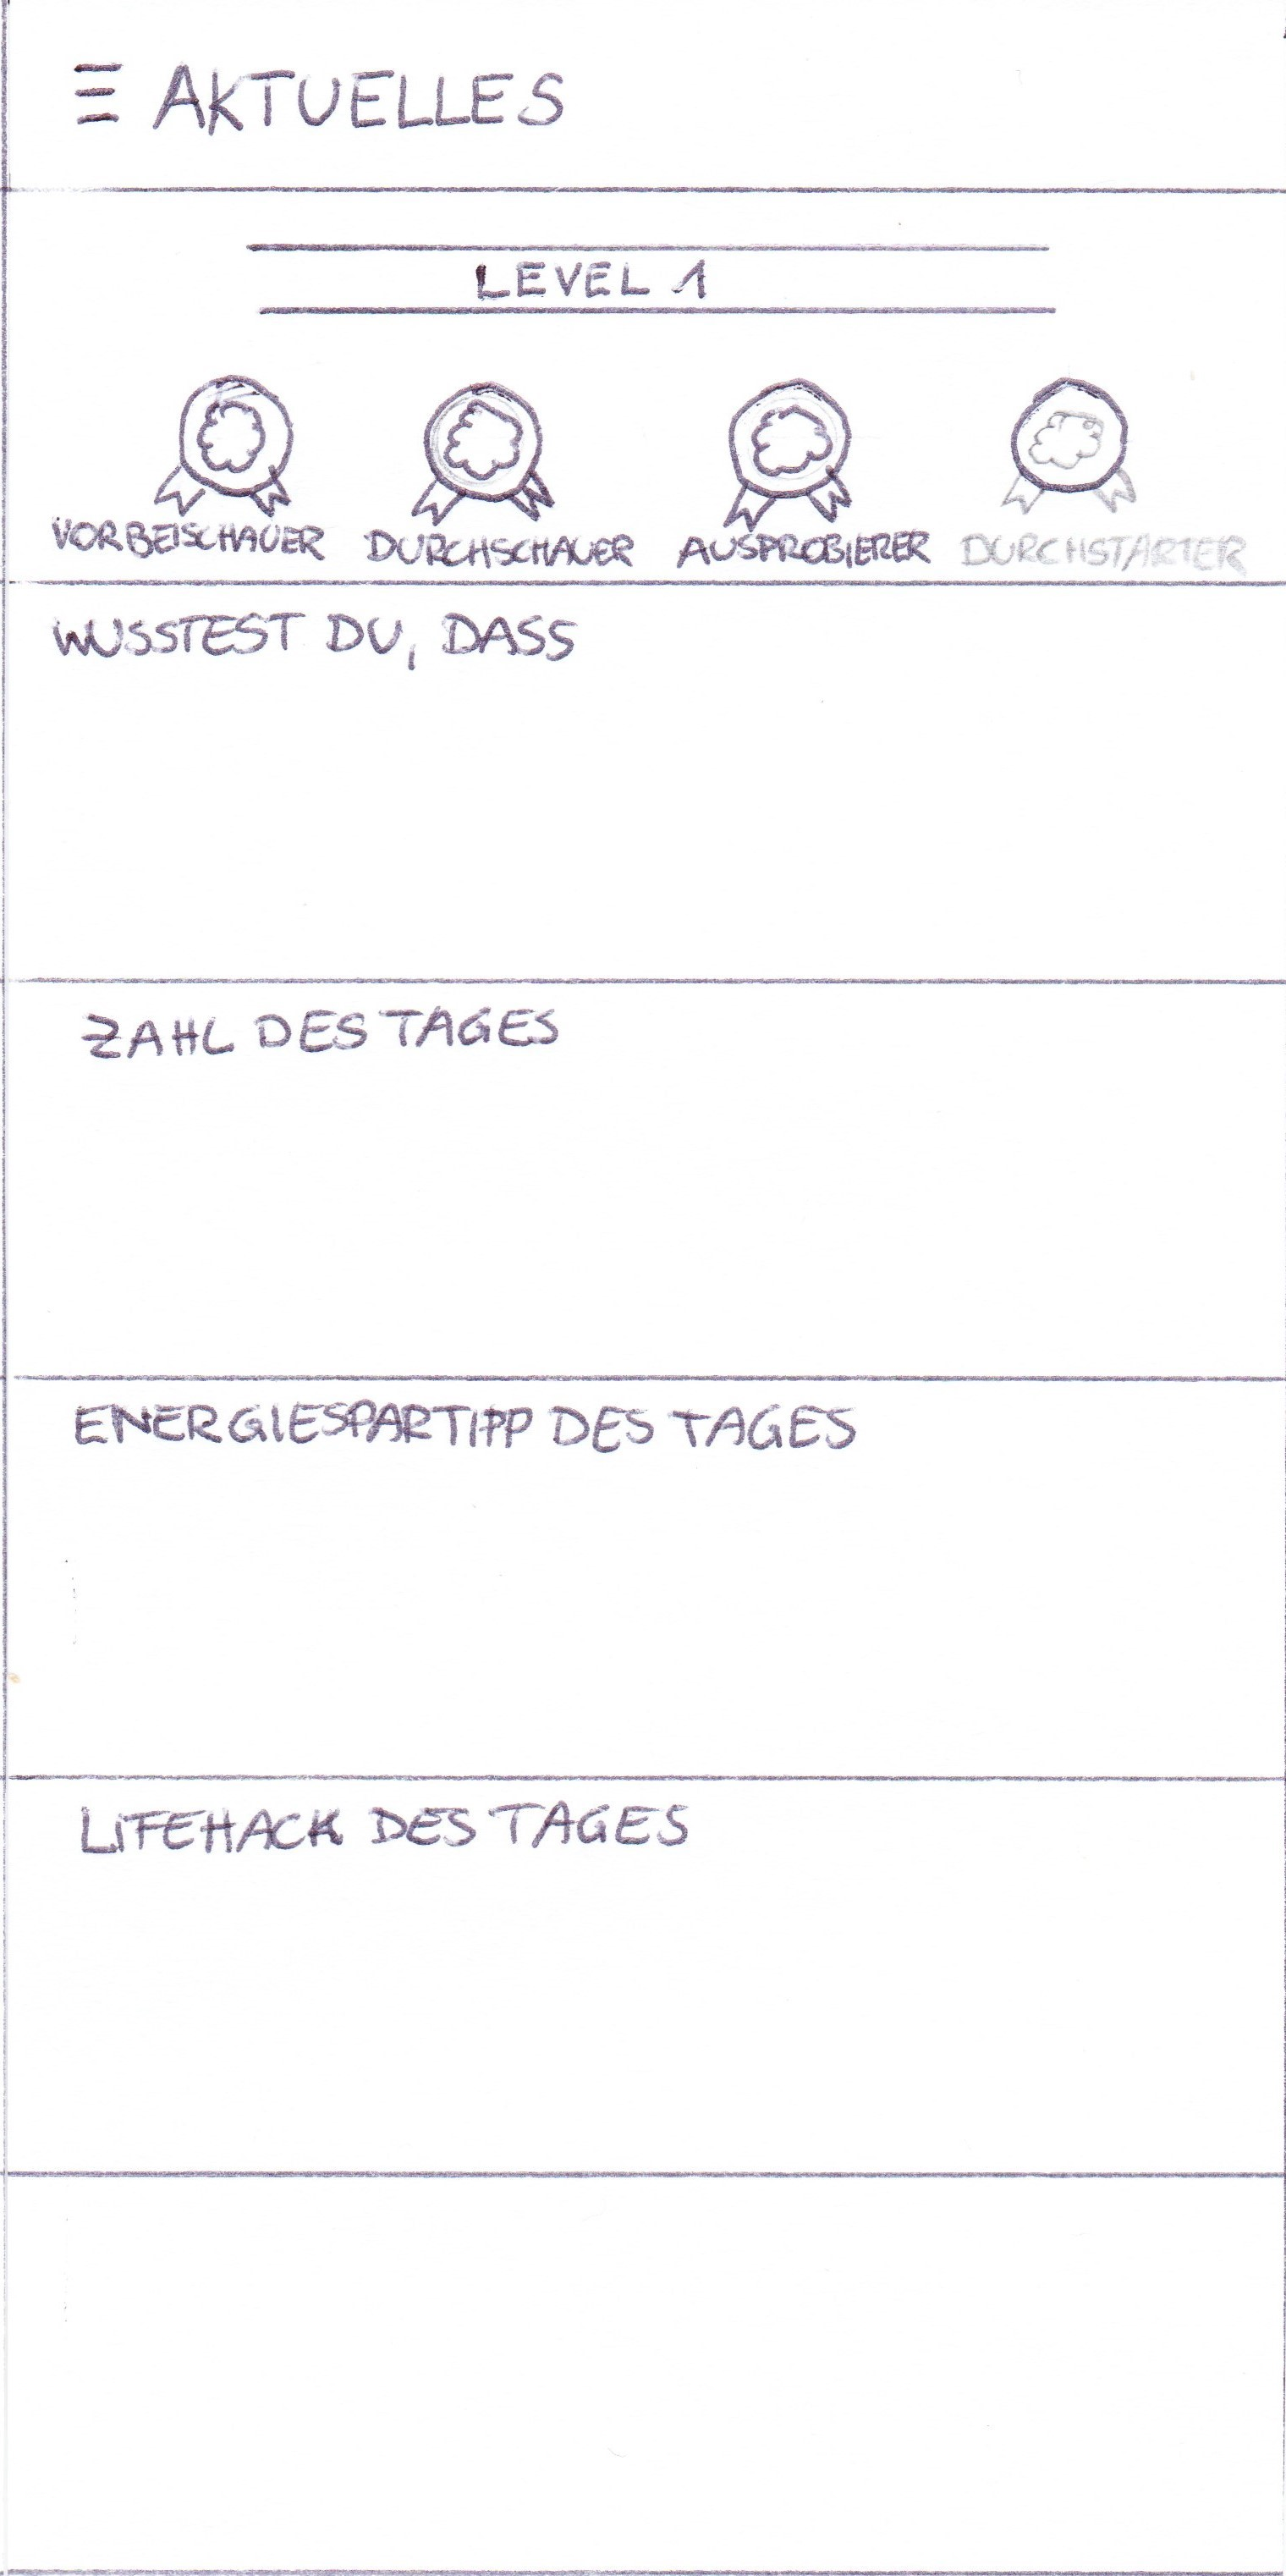
\includegraphics[width=\textwidth]{screens/aktuelles_23}
		\subcaption{Optimizer and Indifferent}
		\label{fig:aktuelles:optimizer}
	\end{subfigure}
	\caption{The proposed screen for the latest topics}
	\label{fig:aktuelles} % \label has to be placed AFTER \caption (or \subcaption) to produce correct cross-references.
\end{figure}

\subsection*{Guideline 3: Use the thrive of Hedonists to program and provide projects for them}

Depending on the user type the measurement unit is changed and the value converted accordingly. The electricity and heating consumption is shown in kWh for Professionals and Hedonists and in Euro for Optimizers and Indifferents. The same counts for consumption of water. Optimizers and Indifferents prefer the measurement unit Euro to cubic meter.

\textbf{Evidence} \quad Tunnelling, as mentioned before in ~\nameref{subsec:primaryTask}, is great because it guides a user through an attitude change process. This design principle is used for the projects, as it shows a Step-by-Step guide of what to do in a project. The test user of the Hedonist user segment very much liked the projects section.

\begin{itemize}
	\item As a Hedonist I love to do projects where I can save energy in the long run.
	\item As a Hedonist I don't like to follow tips that limit my comfort.
\end{itemize}

\section{Statistics}

Figure~\ref{fig:statistik} shows the statistics screens where a user can monitor the latest consumption of electricity, heating, water and the emitted CO2 value. Day, week, month or year are periods of time can be selected. In every period values can be compared to previous consumption rates, see Figure~\ref{fig:statistik:mitvergleich}.

\textbf{Improvements} \quad An improvement mentioned by a Professional was to split up the statistics into consumption statistics and quality statistics. The latest can then e.g. show the room temperature, the air quality in CO2 or the air humidity. The Optimizer wished for a possibility to switch to Euro. Showing an area in the diagram that indicates with colours where the "good" and the "bad" range lies, was wished by an Indifferent test user.

\begin{figure}[h]
	\centering
	\begin{subfigure}[b]{0.24\columnwidth}
		\centering
		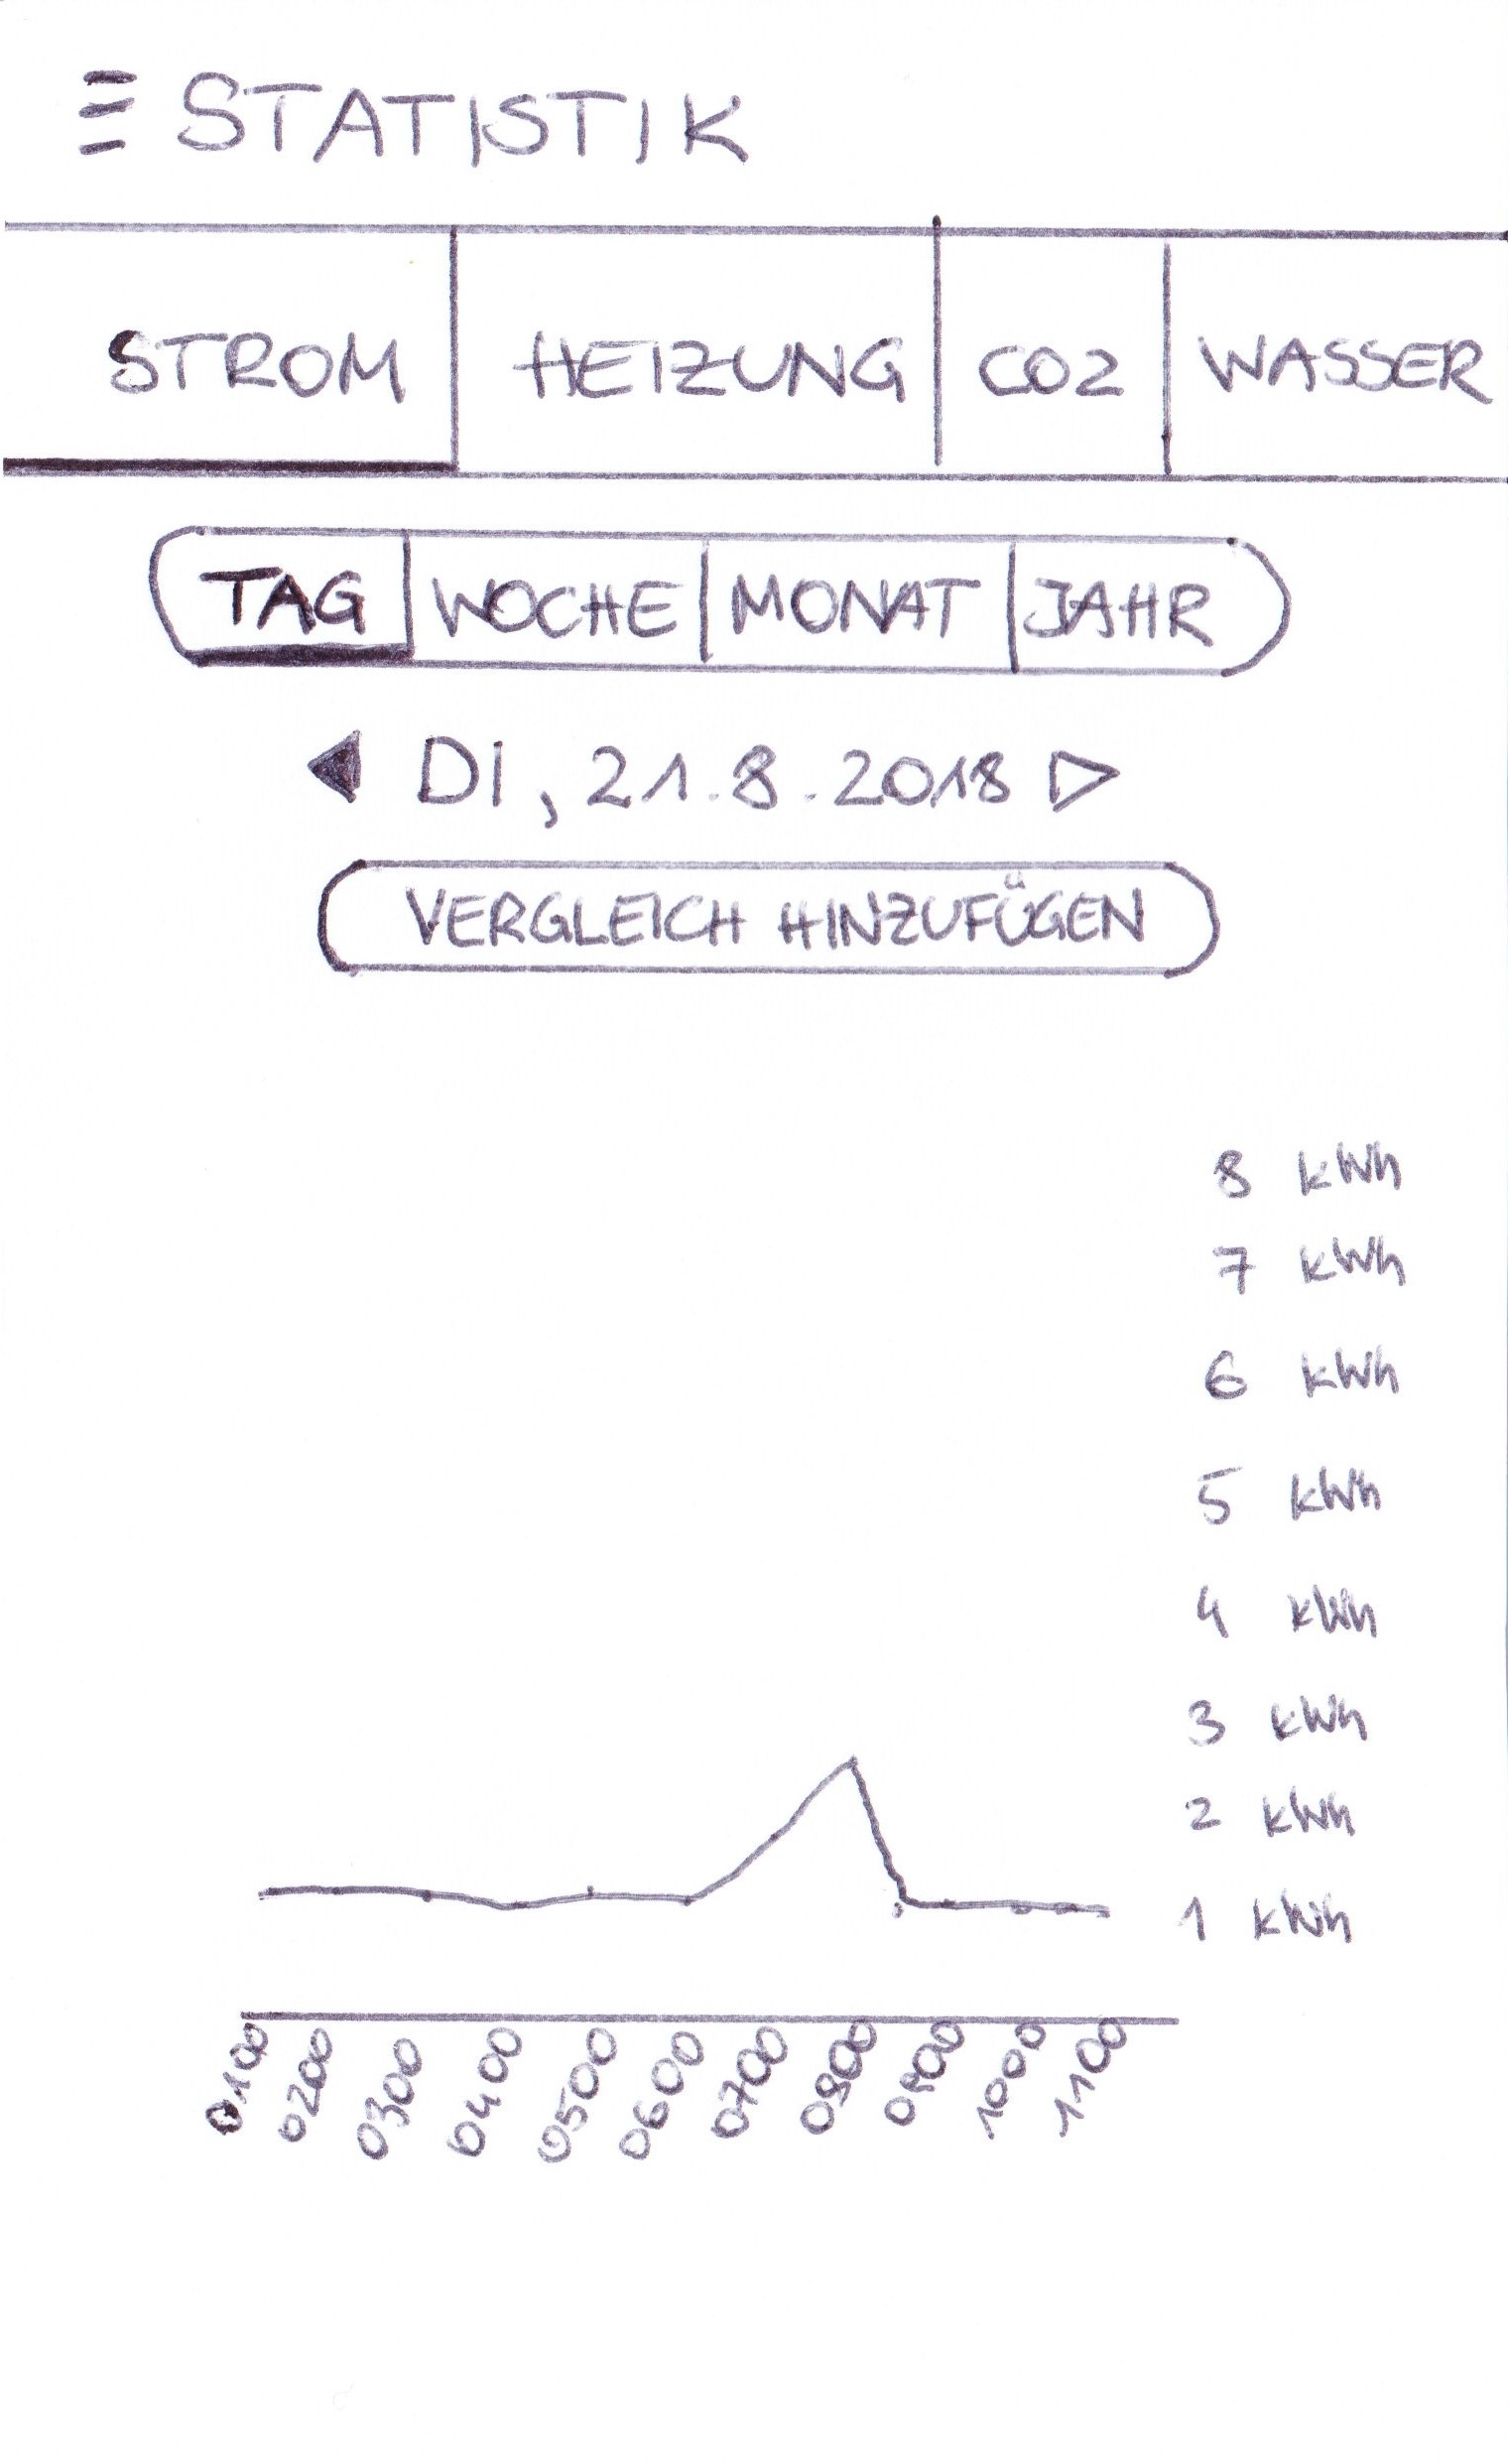
\includegraphics[width=\textwidth]{screens/Statistik_1234}
		\subcaption{Professional and Hedonist}
		\label{fig:statistik:ohnevergleich}
	\end{subfigure}
	\begin{subfigure}[b]{0.24\columnwidth}
		\centering
		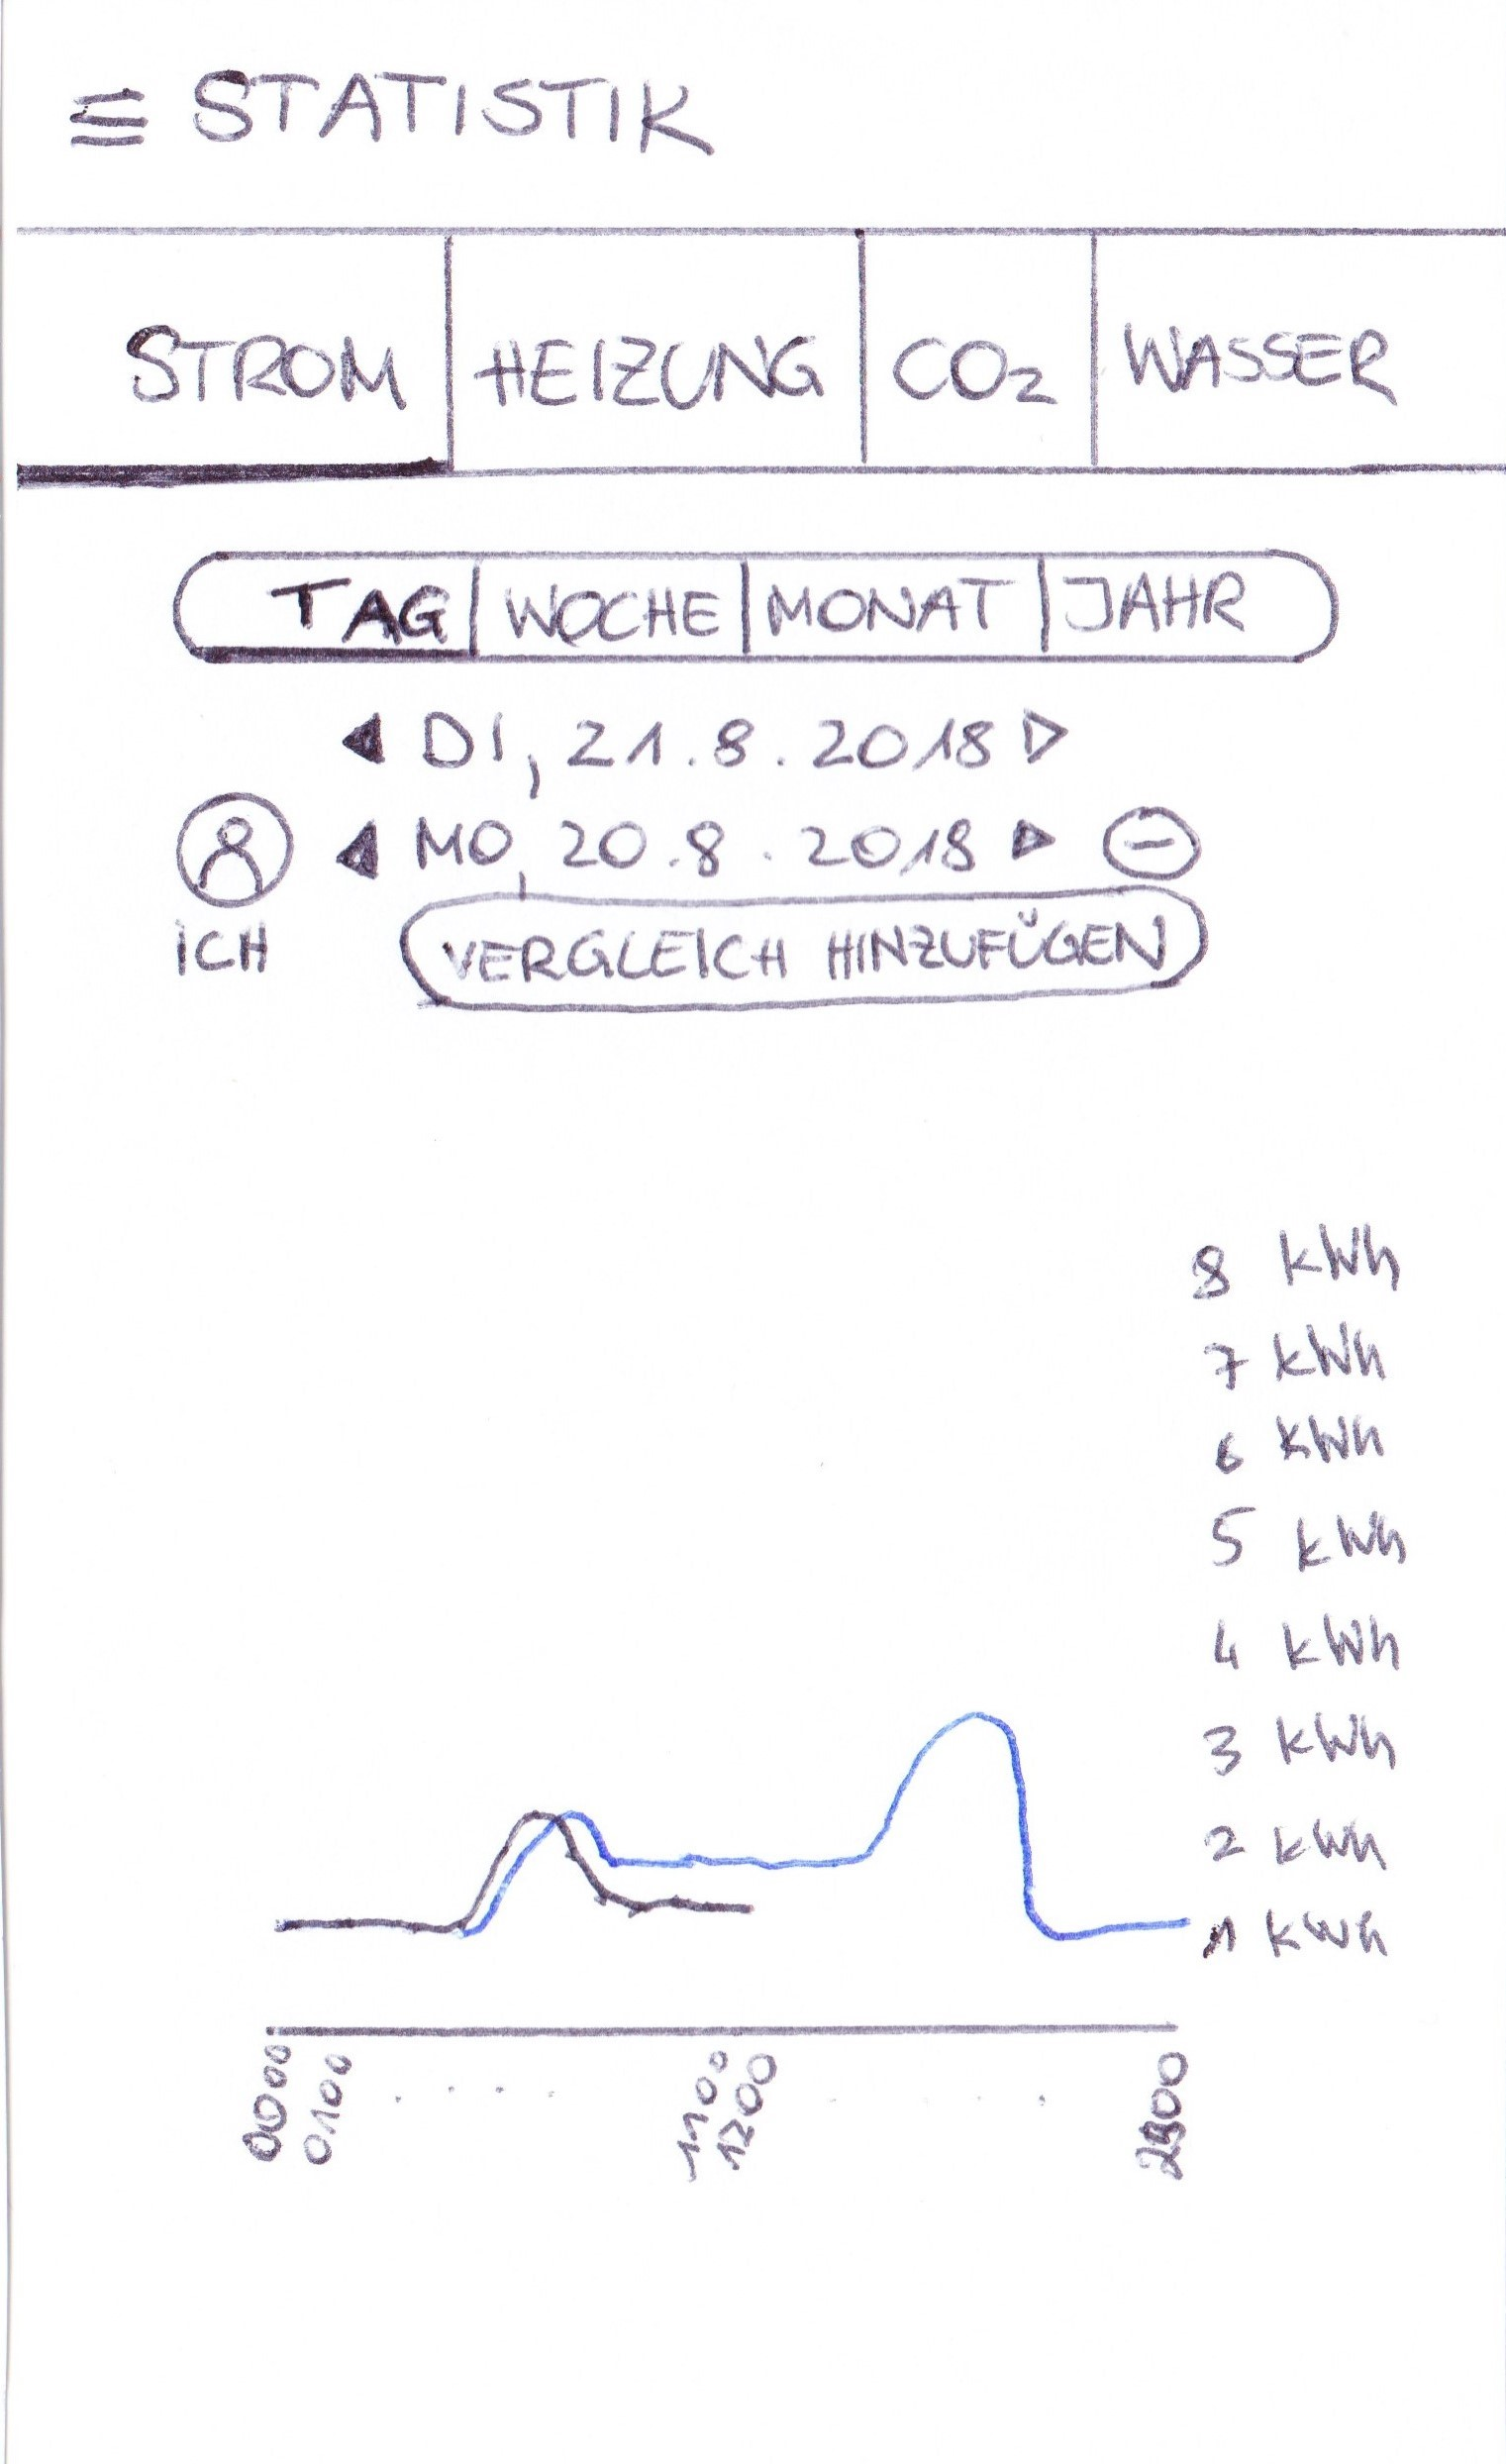
\includegraphics[width=\textwidth]{screens/Statistik_Vergleich}
		\subcaption{Optimizer and Indifferent}
		\label{fig:statistik:mitvergleich}
	\end{subfigure}
	\caption{The proposed screens for statistics}
	\label{fig:statistik} % \label has to be placed AFTER \caption (or \subcaption) to produce correct cross-references.
\end{figure}

\subsection*{Guideline 4: Provide diagrams to monitor the consumption rate for Professionals, Optimizer, Indifferents and Hedonists}

Making use of diagrams to show consumption and history data and provide the possibility to switch between different time intervals.

\textbf{Evidence} \quad The design principle of Self-monitoring, as explained in ~\nameref{subsec:primaryTask}, shall provide users with the possibility to monitor their performance, which is clearly given with diagrams of latest consumption figures. All of the test user mentioned that they like to have a look on past consumption figures.

\section{Equipment control}

All the manageable tools are grouped in the equipment control. The ones that are managed are active and the other ones are greyed out, as pictured in Figure~\ref{fig:equipment:overview}. Profiles can be selected and are adaptable.

\textbf{Improvements} \quad All test users proposed to use other wording for the profile. "Home" instead of "Home-office" because it is not clear that "Home-office" can also be used at weekend. Instead of "Goal temperature" the term "Manually" was mentioned. One Professional noticed an obvious lack of the equipment control: the absence of weekly profiles. The adding of who has changed the value at last time was wished from a Hedonist participant.

\begin{figure}[h]
	\centering
	\begin{subfigure}[b]{0.24\columnwidth}
		\centering
		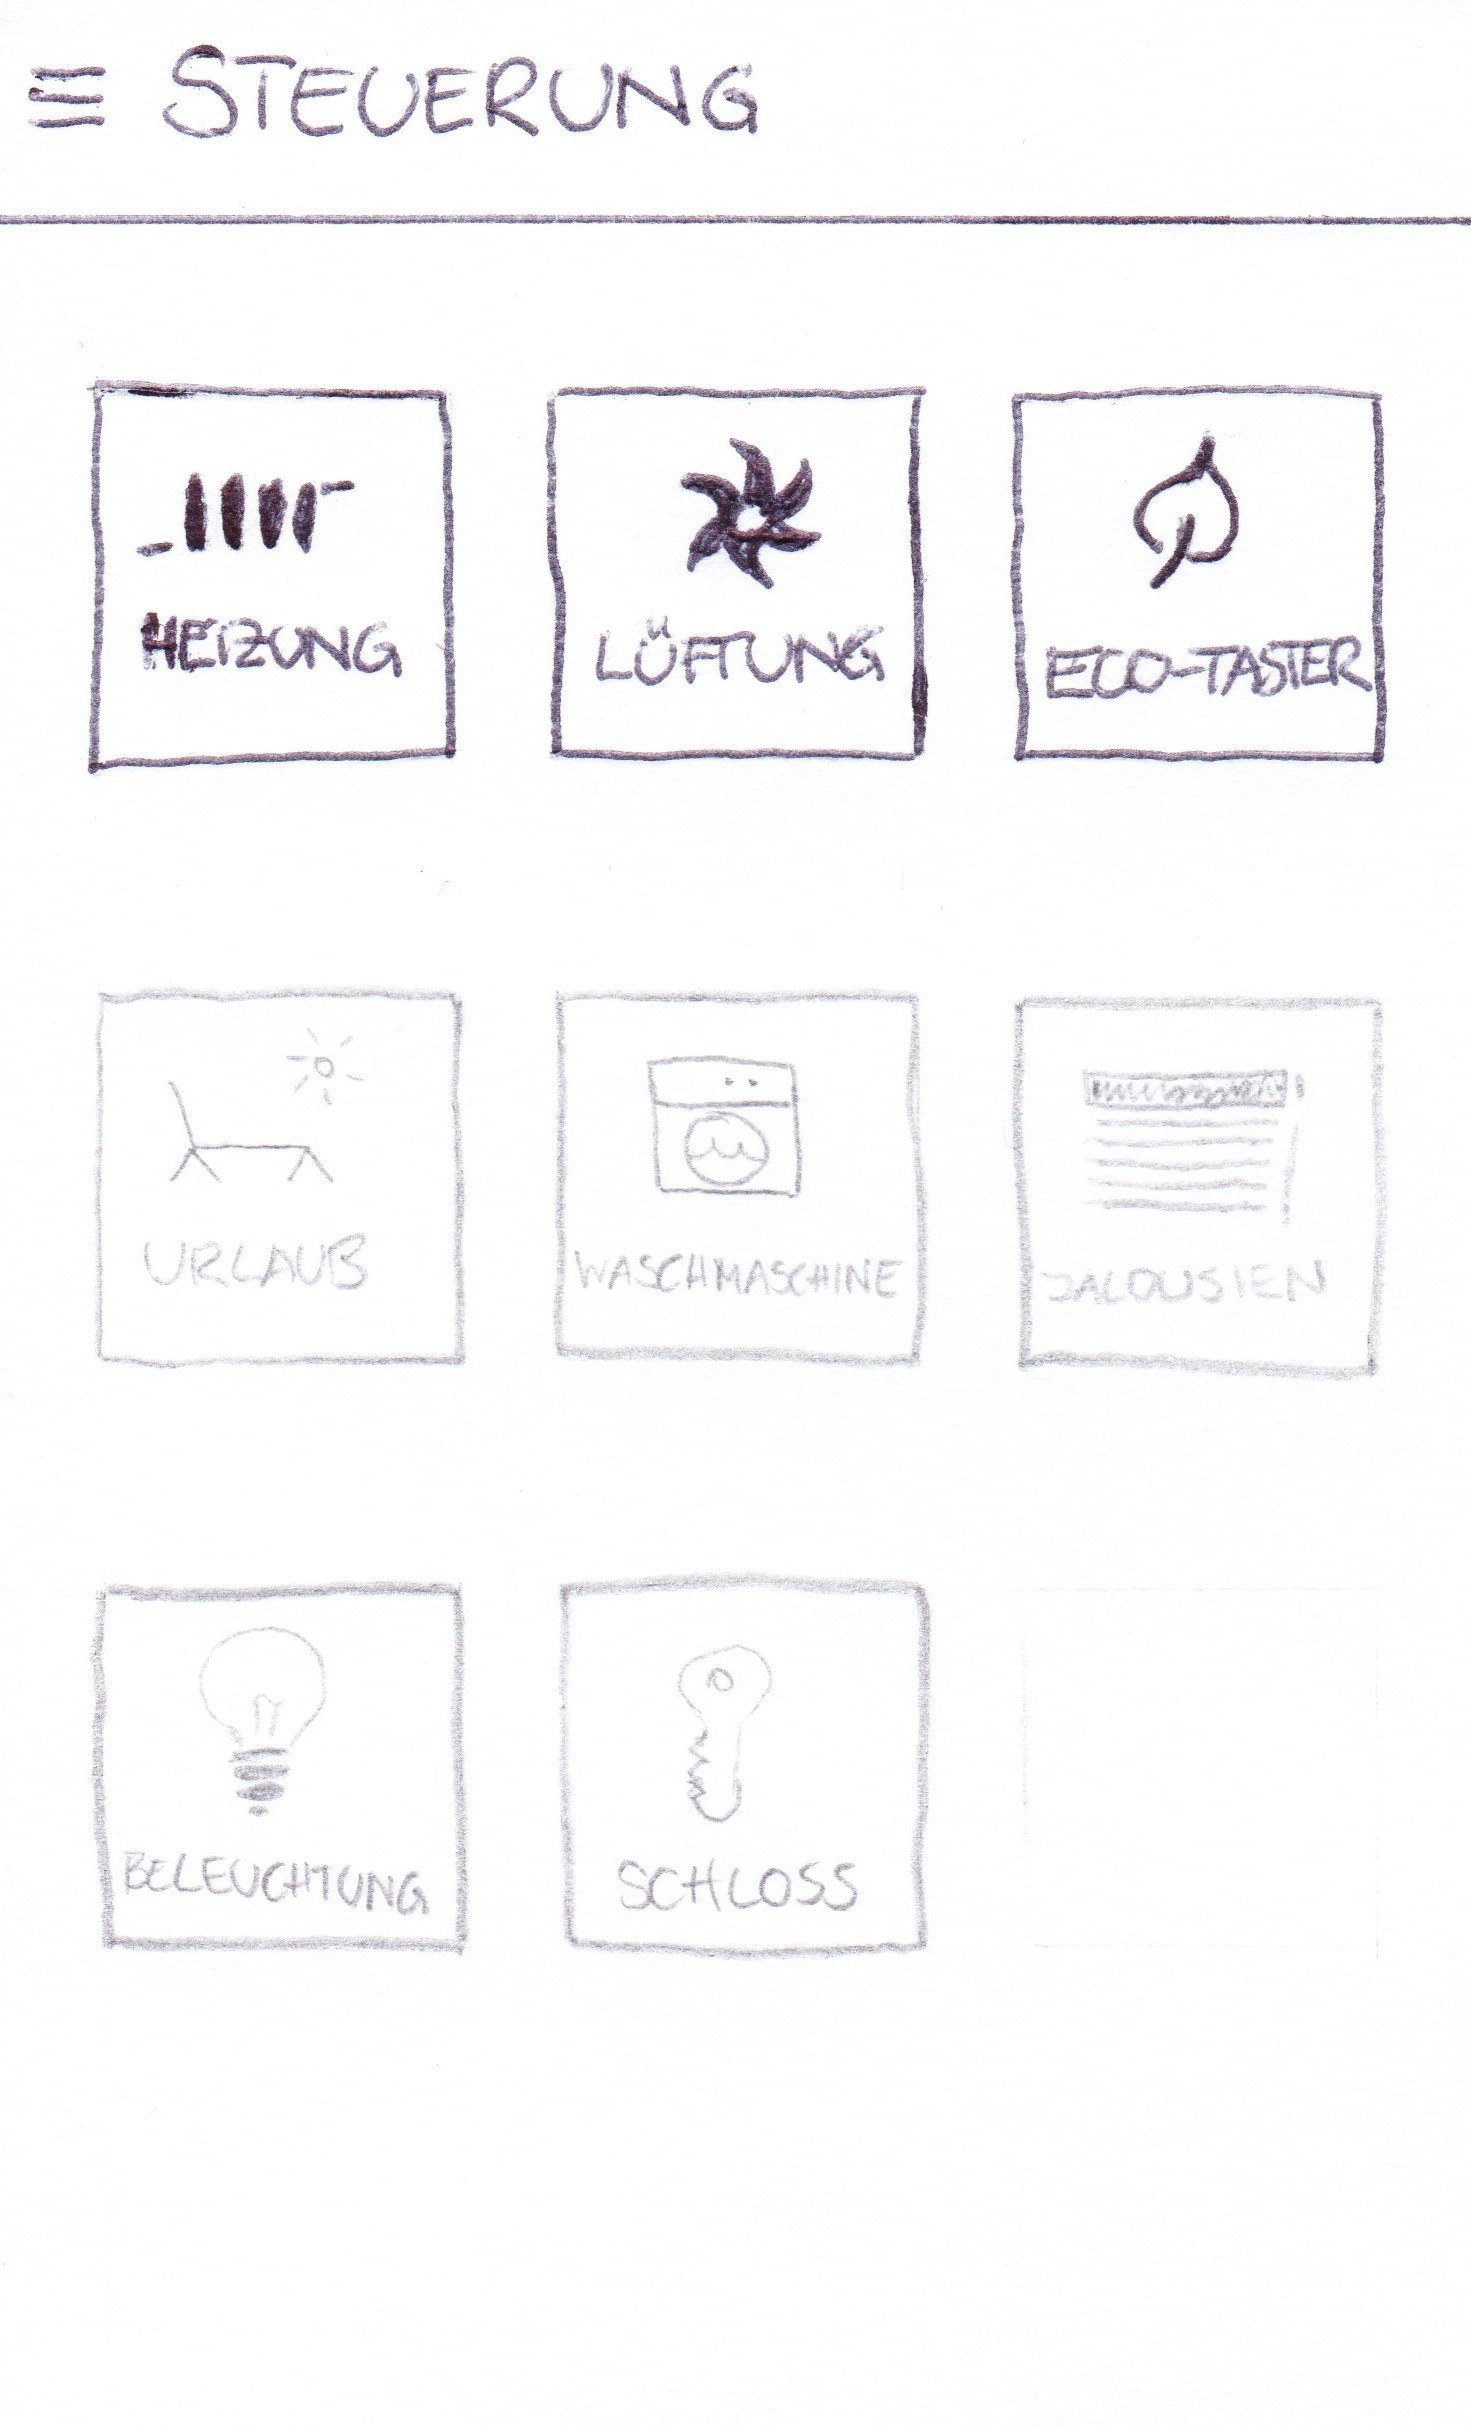
\includegraphics[width=\textwidth]{screens/Steuerung_1234}
		\subcaption{Professional and Hedonist}
		\label{fig:equipment:overview}
	\end{subfigure}
	\begin{subfigure}[b]{0.24\columnwidth}
		\centering
		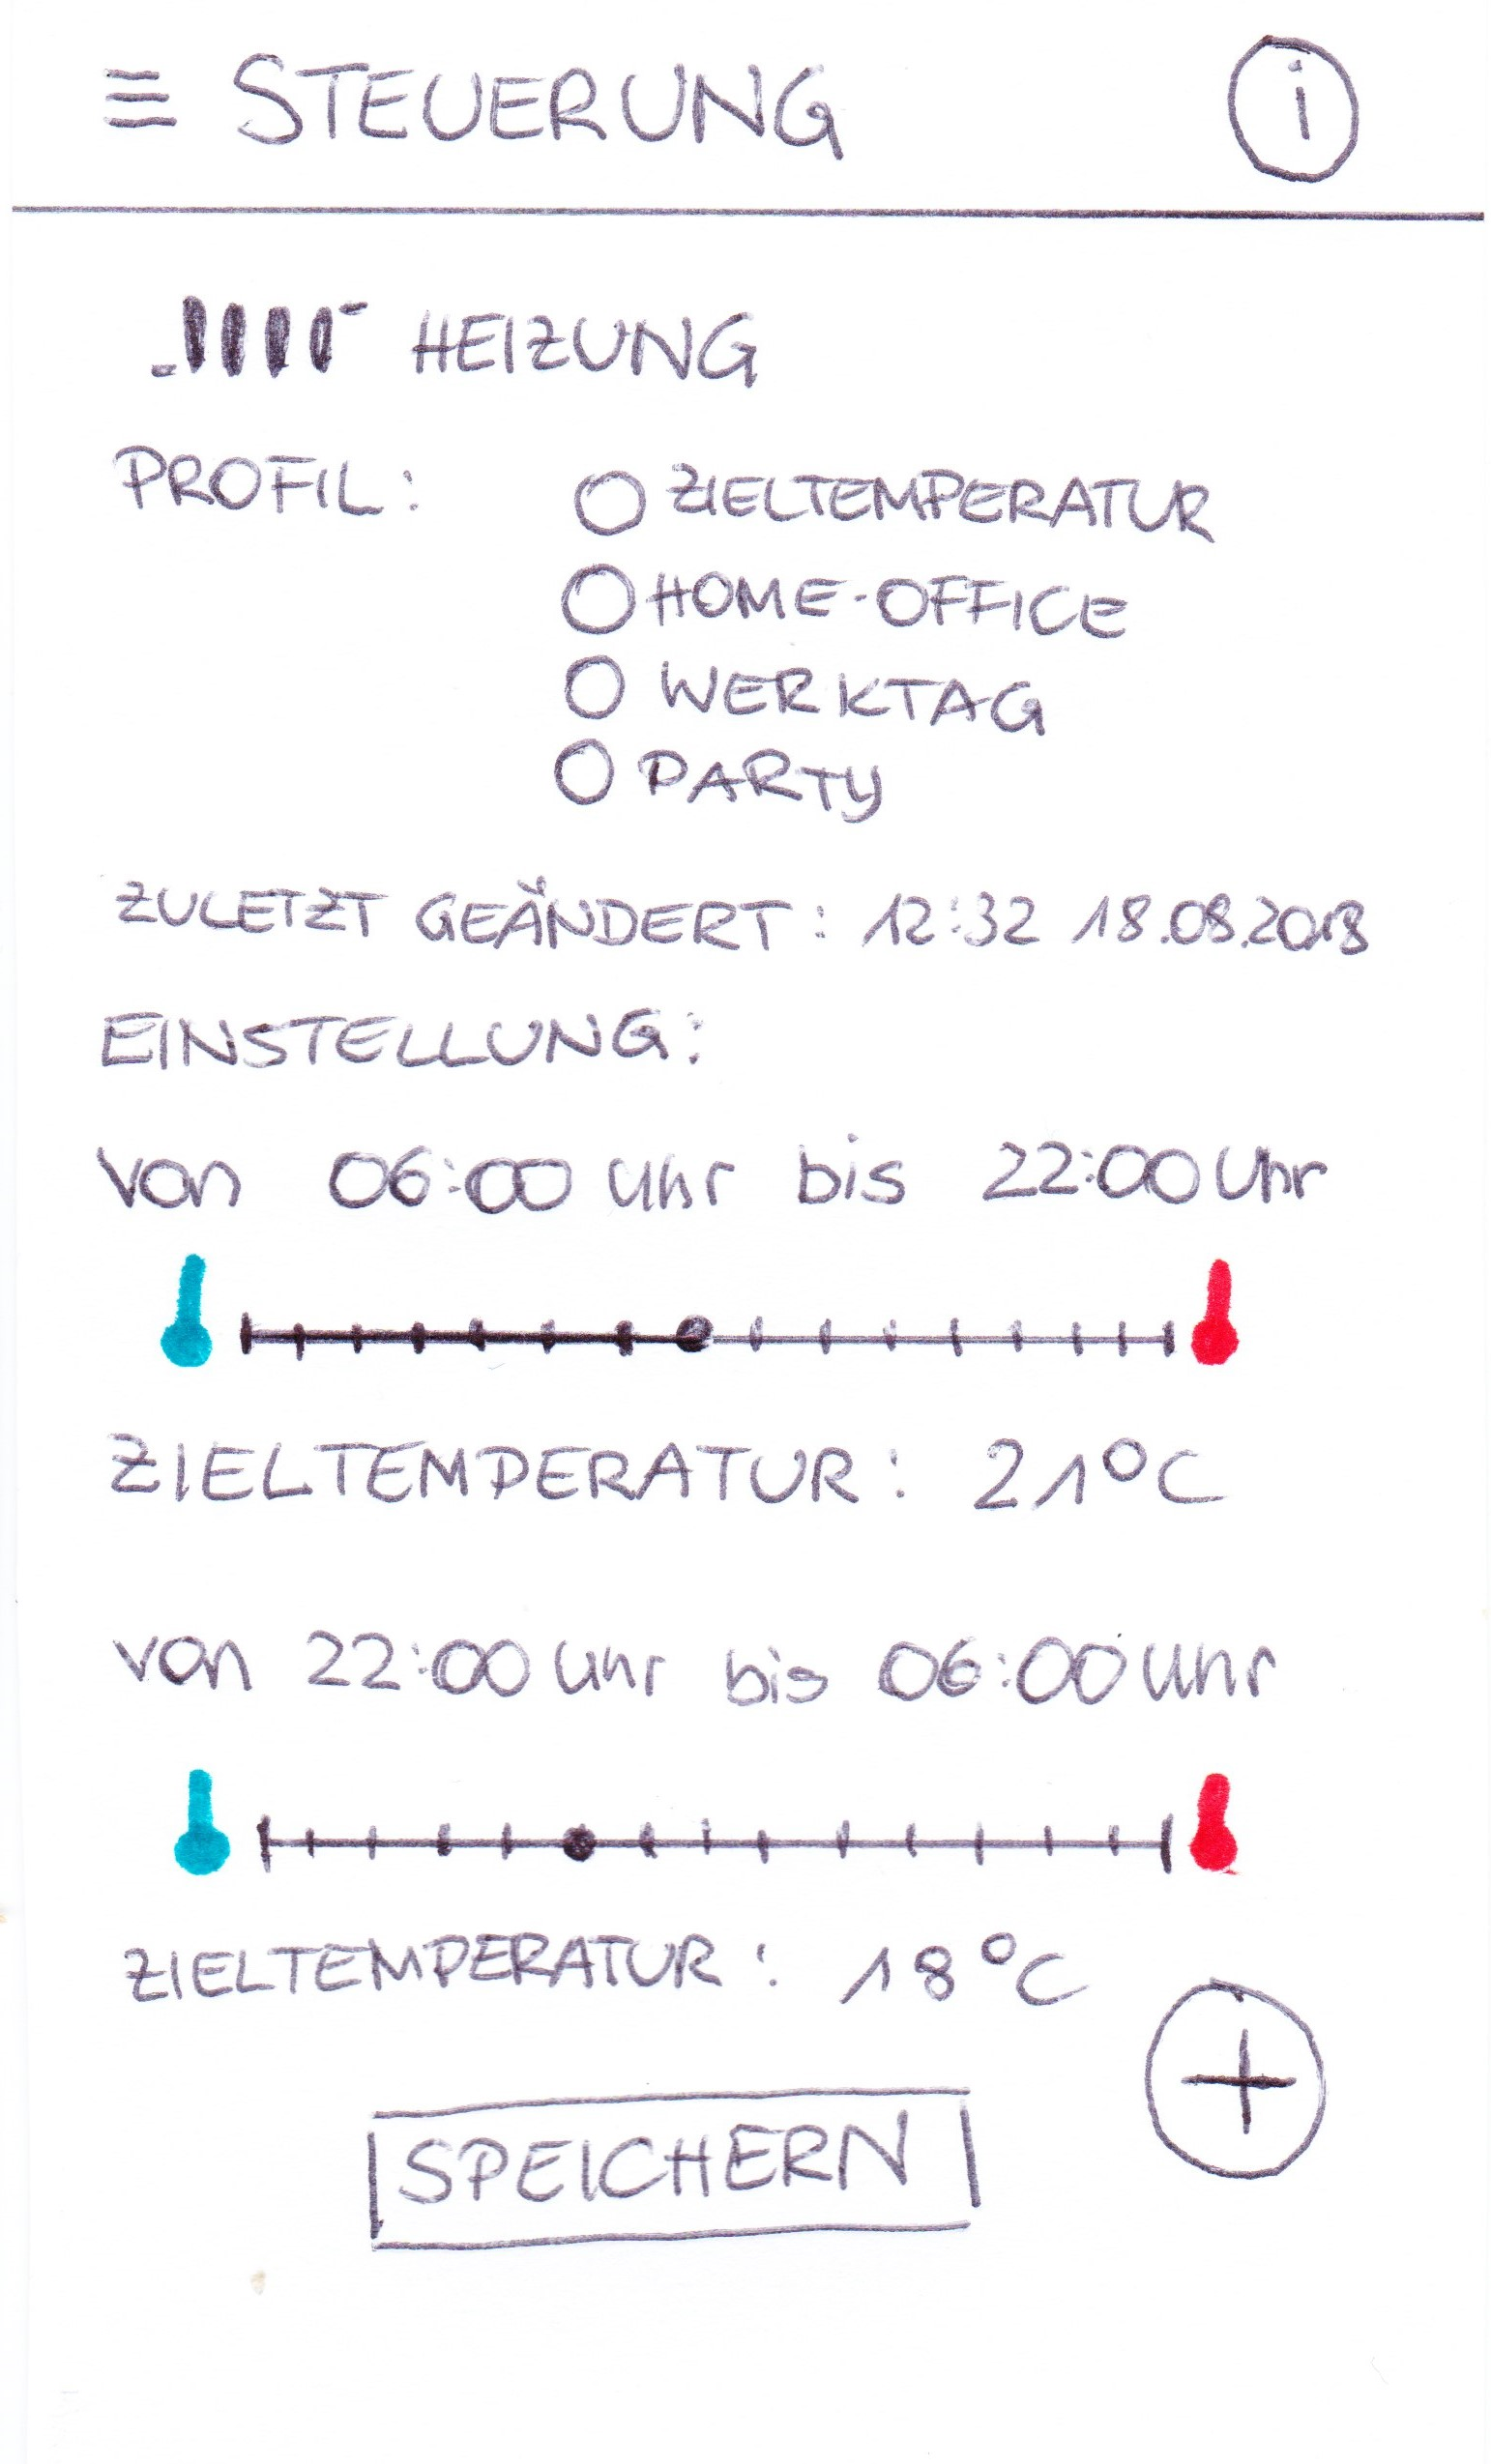
\includegraphics[width=\textwidth]{screens/Steuerung_Heizung}
		\subcaption{Optimizer and Indifferent}
		\label{fig:equipment:profile}
	\end{subfigure}
	\caption{The proposed screens for equipment control}
	\label{fig:equipmentcontrol} % \label has to be placed AFTER \caption (or \subcaption) to produce correct cross-references.
\end{figure}

\section{Comparison of Savings}

Figure~\ref{fig:sparen} shows the screens for the comparison of savings for all user types. The screen for the Professionals, see Figure~\ref{fig:sparen:professional}, provides the possibility to compare yourself to the average of your neighbours, to one friend and to see yourself on a rank table. For Optimizers the screen in Figure~\ref{fig:sparen:optimizer} shows that they can set themselves a goal with which they are then compared, leaning on the design principle self-monitoring. Also the total savings of the time interval are shown and an example is given of what can be bought from that amount. A motivation is given by showing the amount that can be saved when the target behaviour is maintained which orientates to the design principle rehearsal. The screen for the Indifferents, pictured in Figure~\ref{fig:sparen:indifferent}, also includes a comparison of the aim and the current value and animates to search for more trophies. Similarly, Hedonists can also see their current value compared to their goal, see Figure~\ref{fig:sparen:hedonist}. Hedonists are then motivated to start or go on with existing projects.

\textbf{Improvements} \quad The Professionals expressed their concerns of sharing their data publicly. They would use the feature of comparing with others but are not ready to make their data available for others. Even here the Professionals preferred kWh to Euros. One Professional criticised the use of too much text and suggested to structure the infos better. The Professionals were the only user group who would like their screen for all the other consumption data. The Optimizer, Indifferents and Hedonists stated that they would like all the four screens for the different tabs. and prefer the mixture of text and values. The Indifferent voiced the concern of feeling supervised when the measured time interval is very short.

\begin{figure}[h]
	\centering
	\begin{subfigure}[b]{0.24\columnwidth}
		\centering
		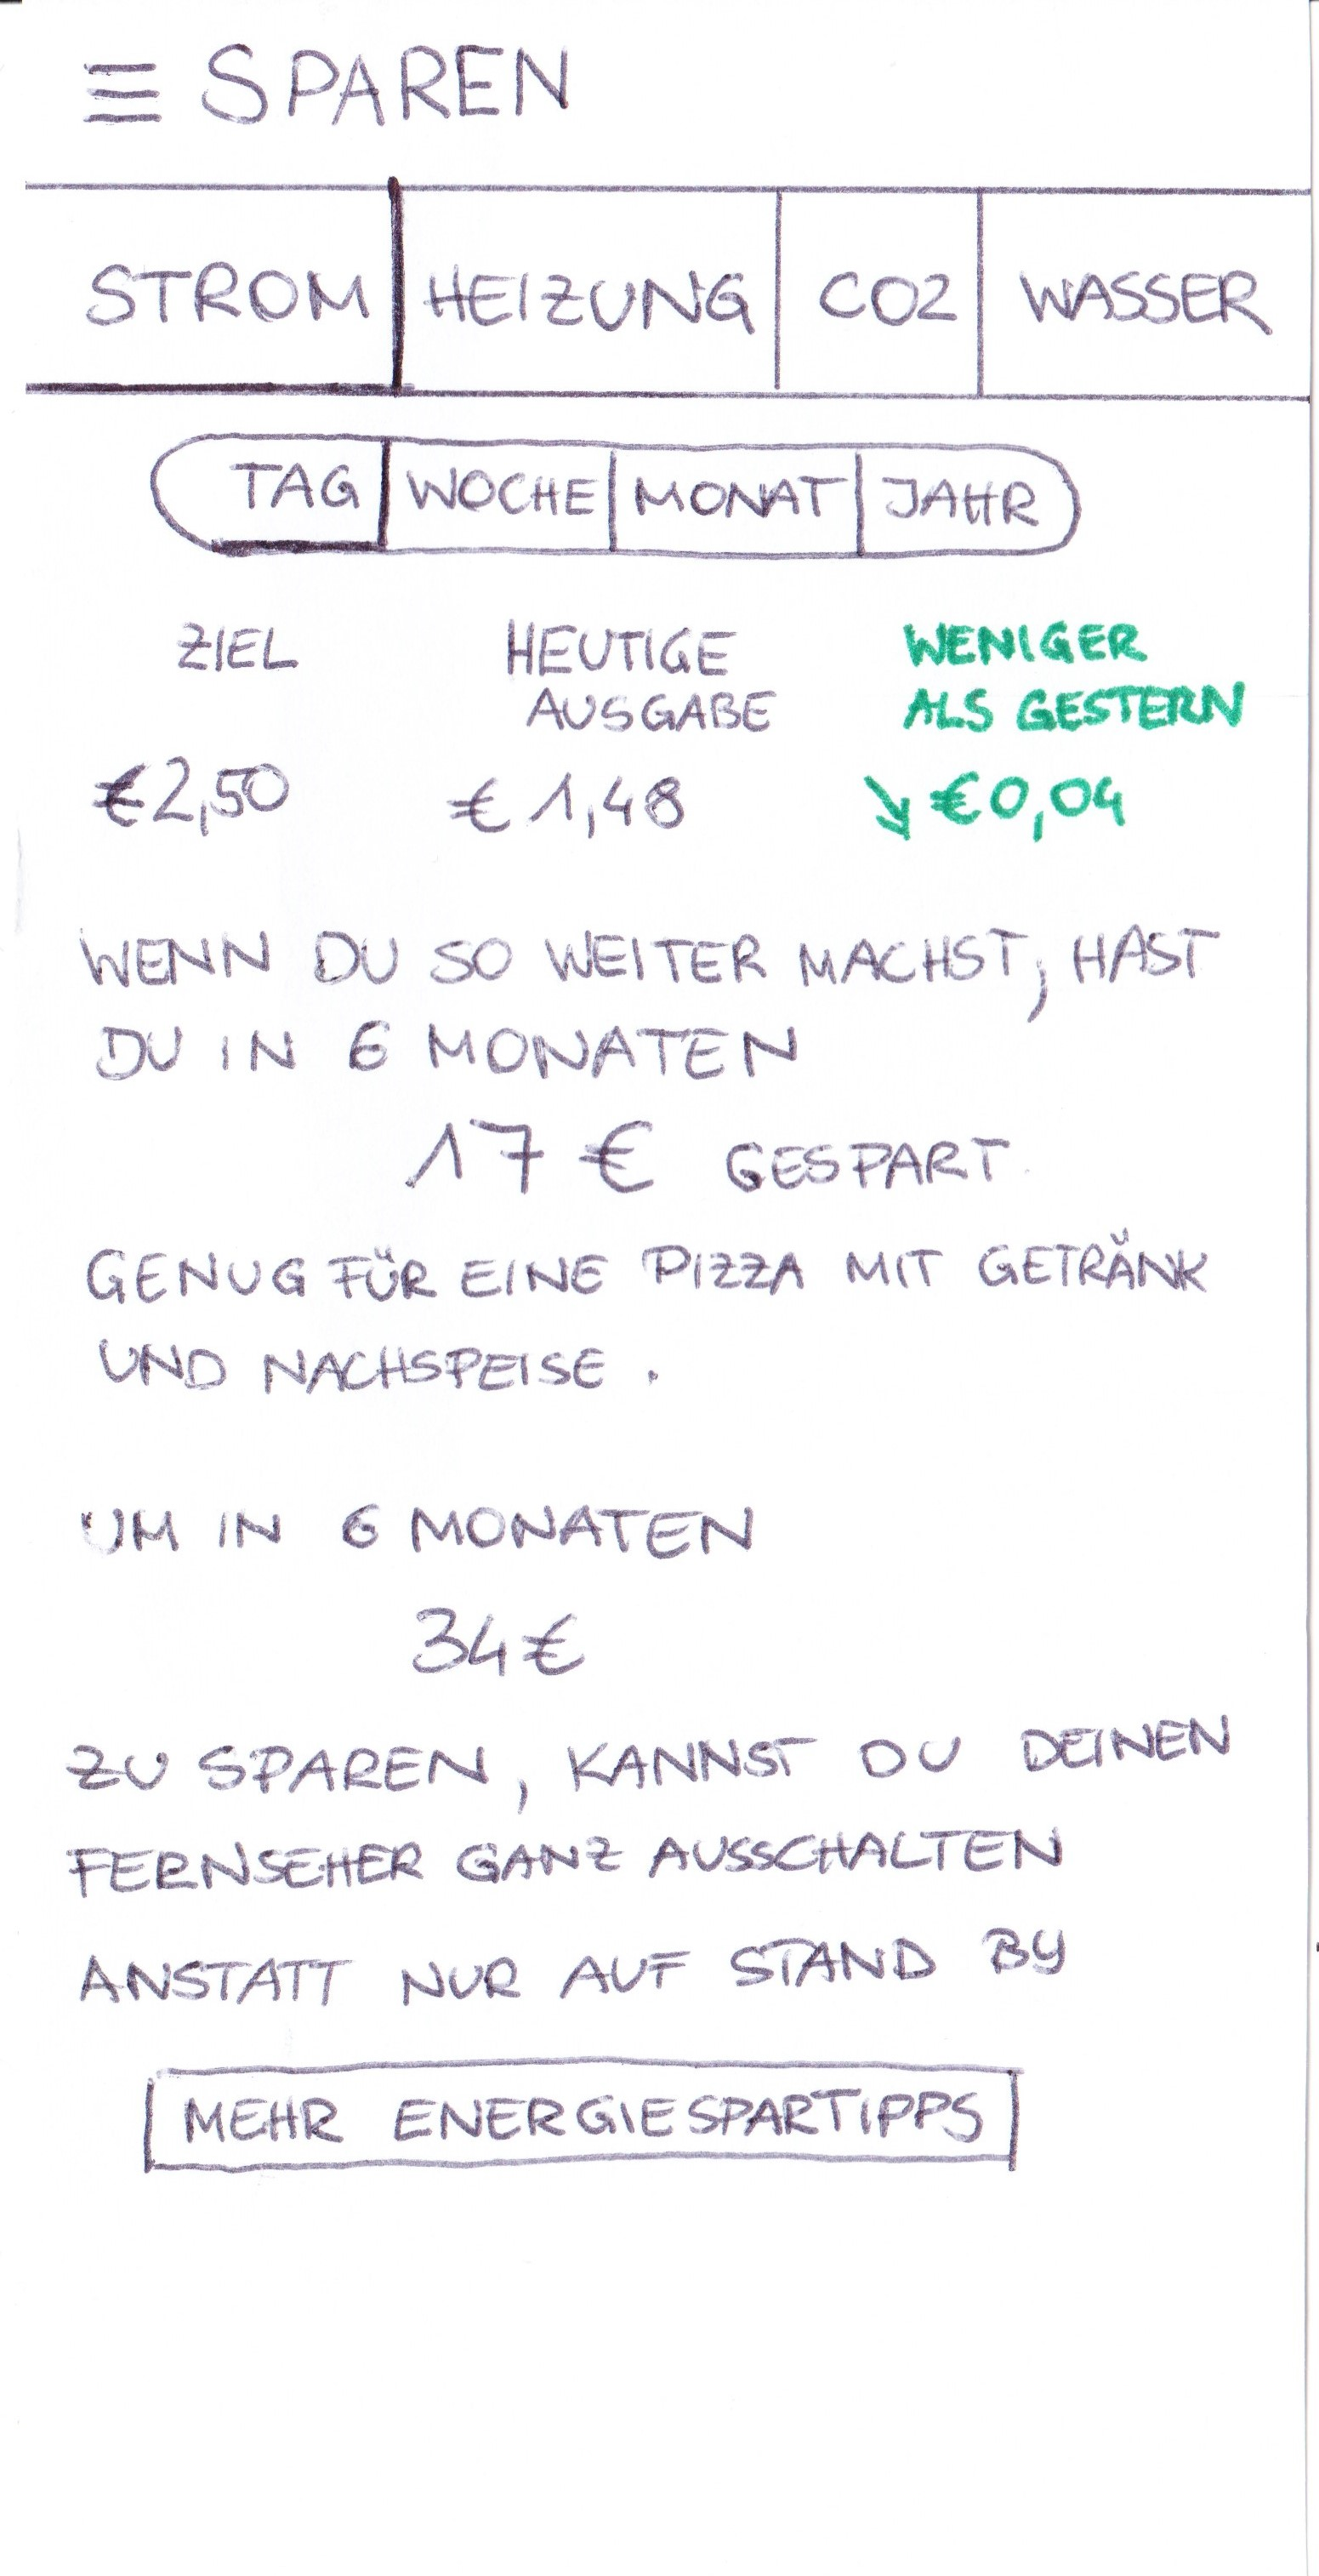
\includegraphics[width=\textwidth]{screens/Sparen_1}
		\subcaption{Professional}
		\label{fig:sparen:professional}
	\end{subfigure}
	\begin{subfigure}[b]{0.24\columnwidth}
		\centering
		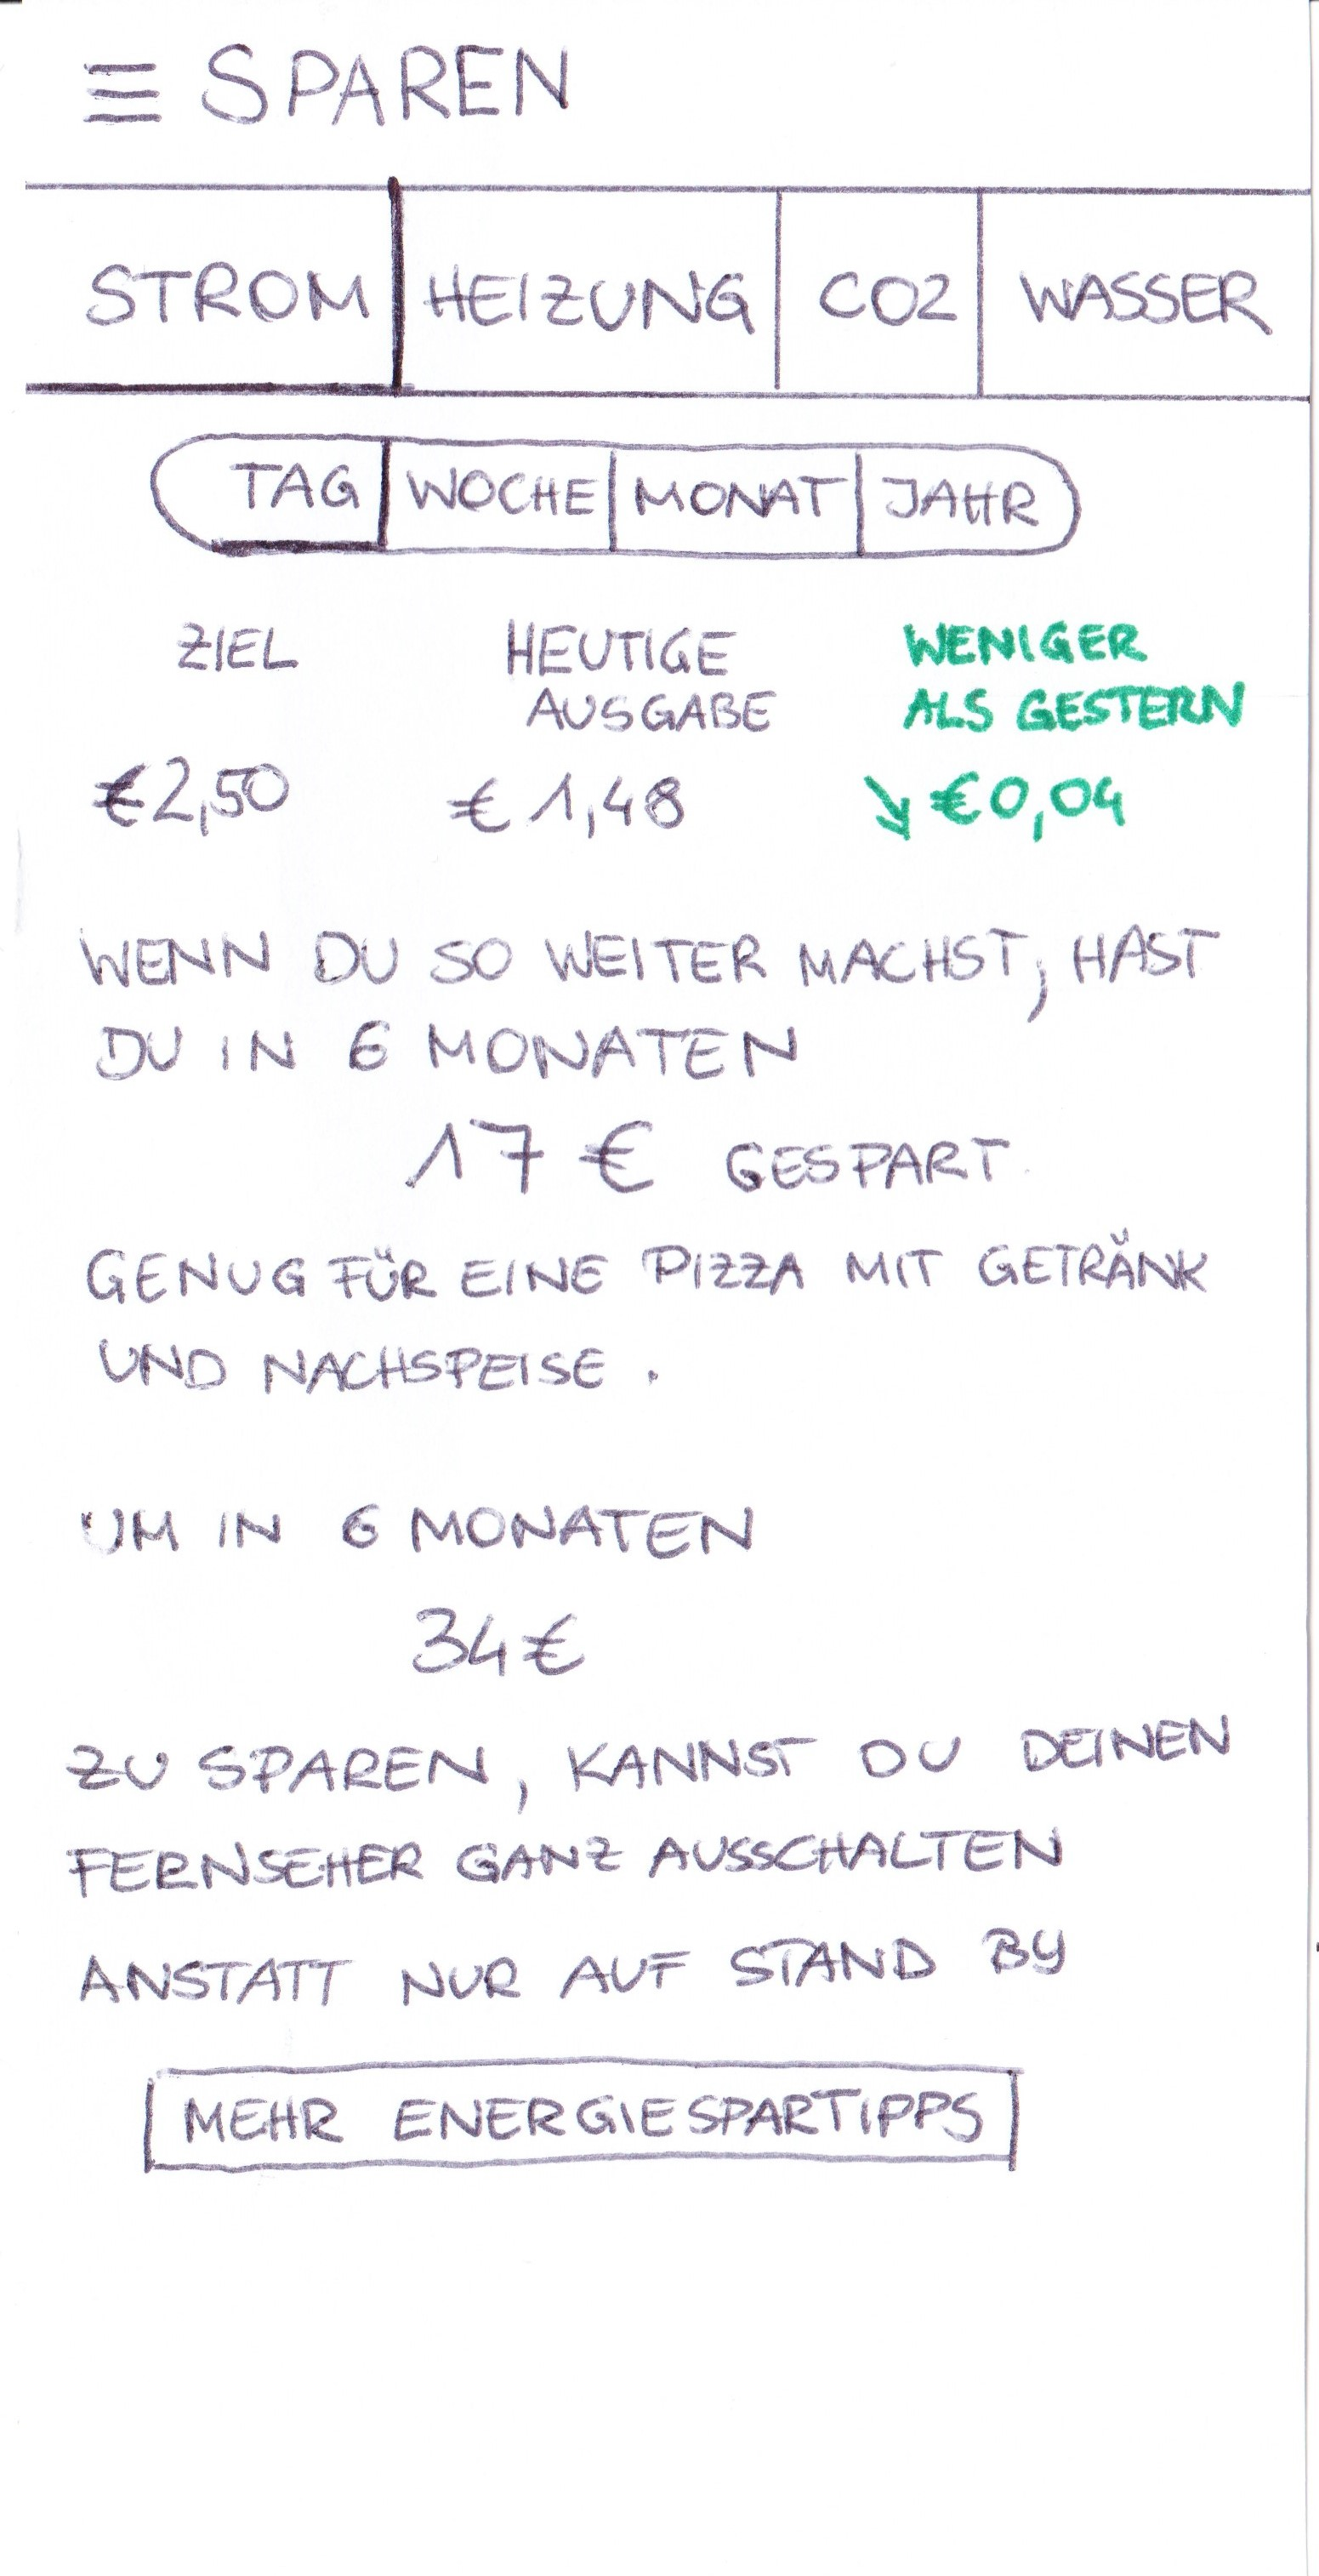
\includegraphics[width=\textwidth]{screens/Sparen_2}
		\subcaption{Optimizer}
		\label{fig:sparen:optimizer}
	\end{subfigure}
	\begin{subfigure}[b]{0.24\columnwidth}
		\centering
		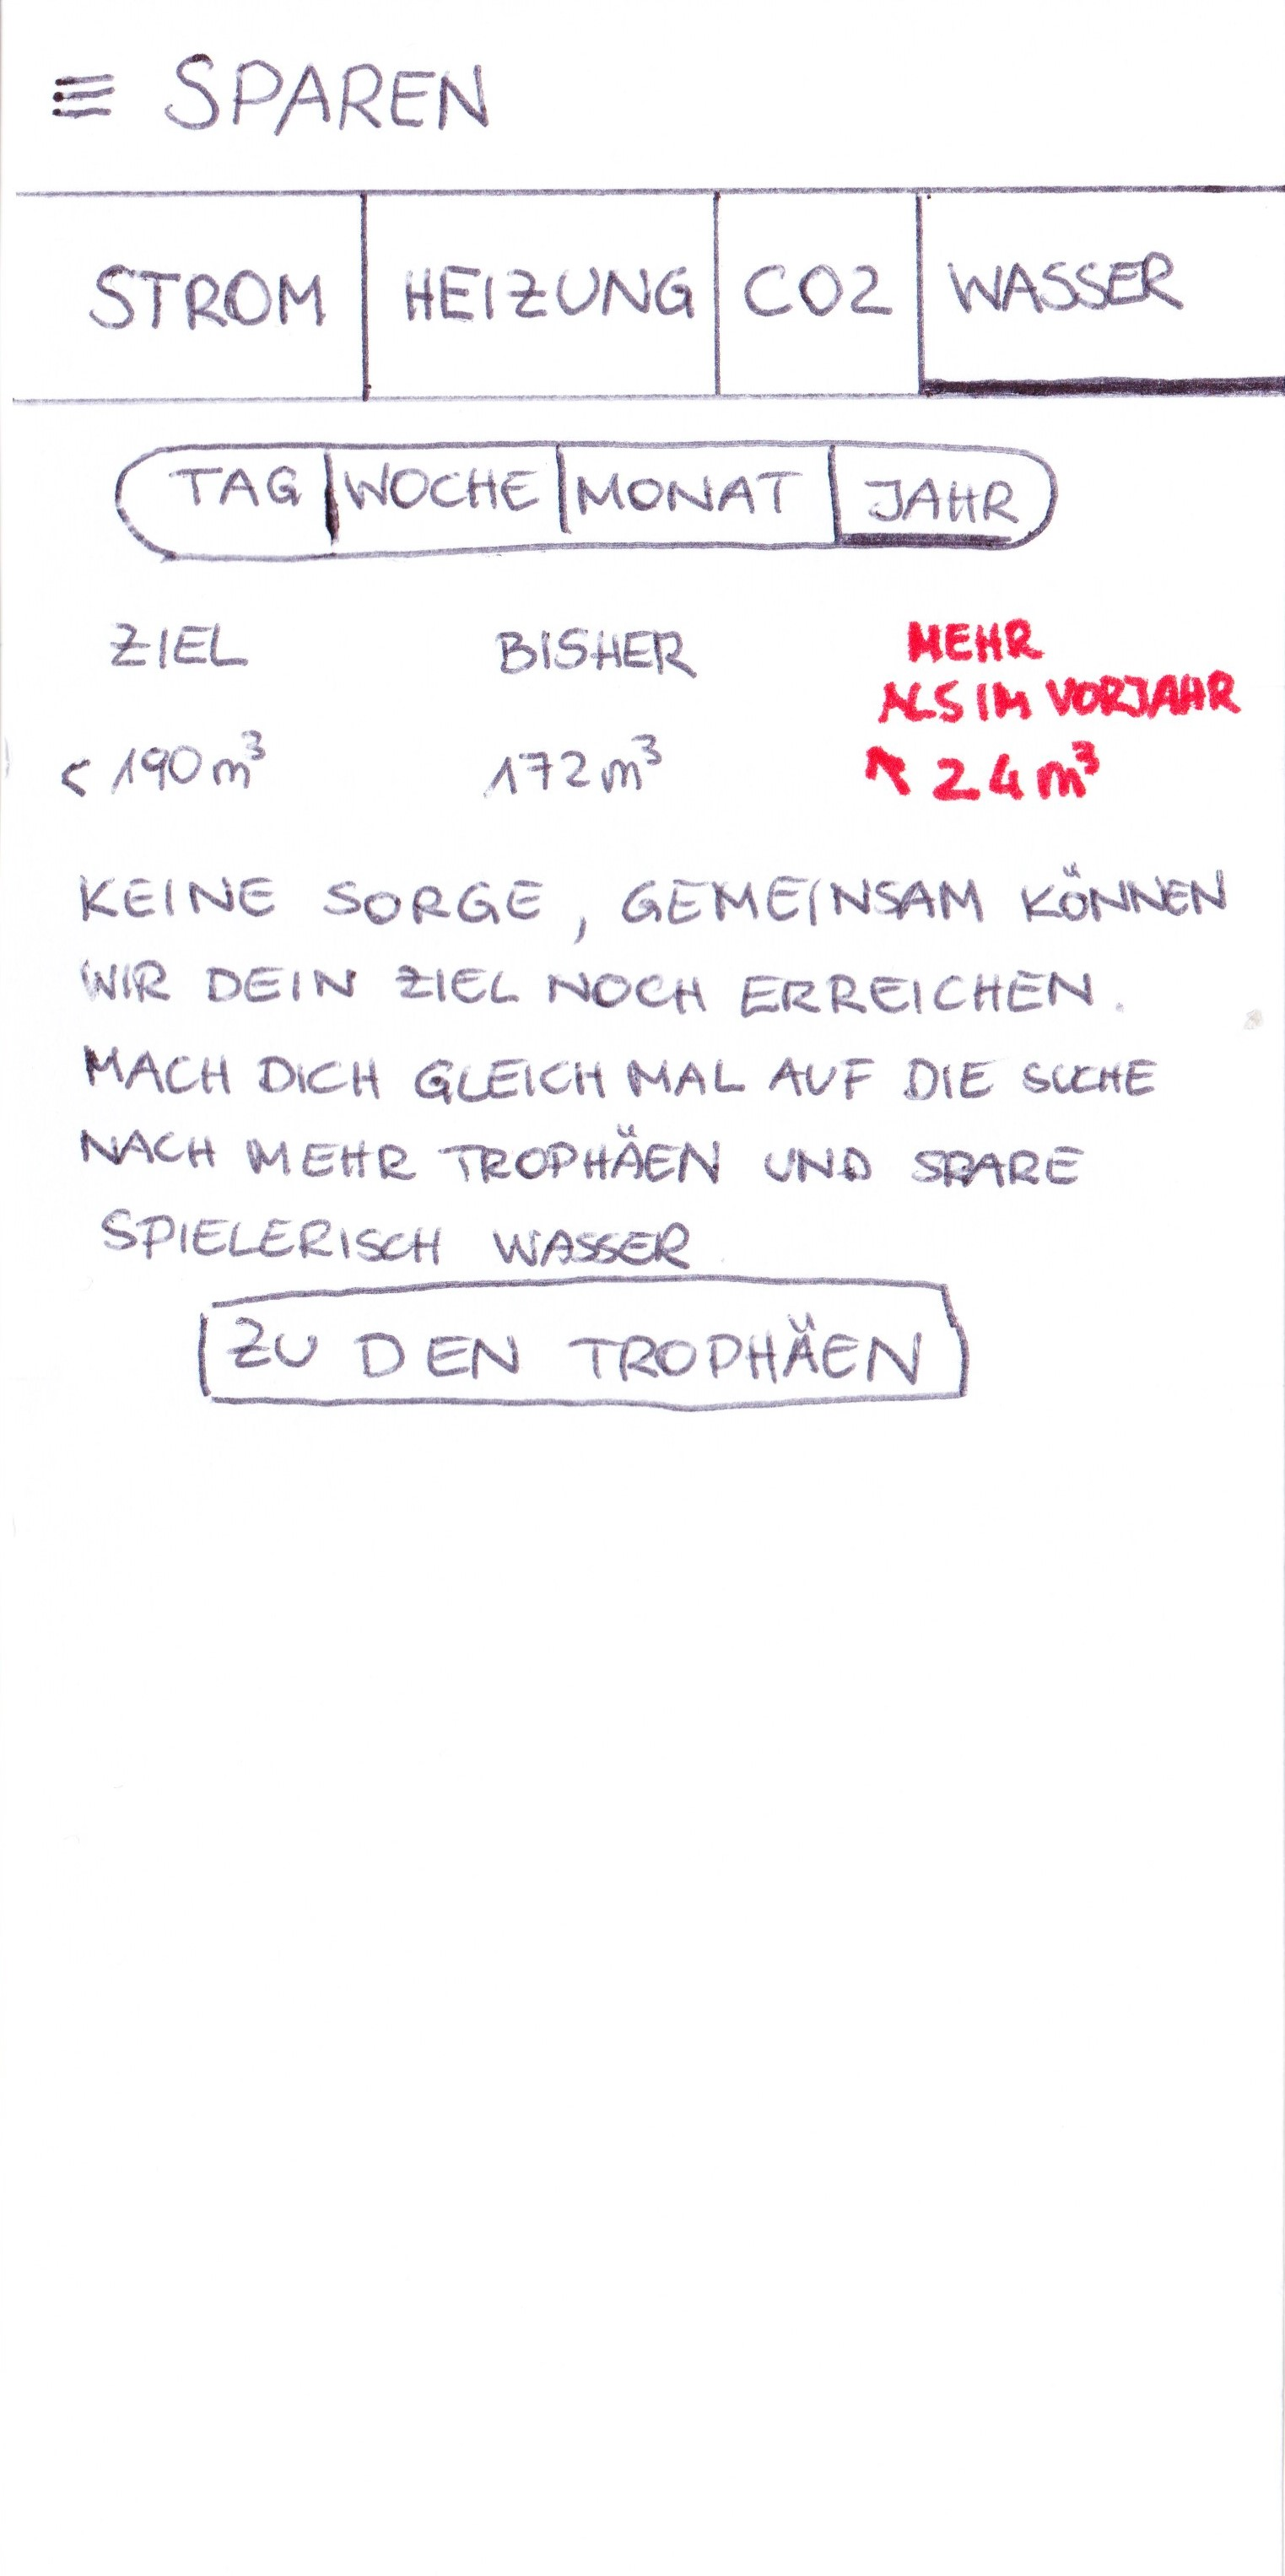
\includegraphics[width=\textwidth]{screens/Sparen_3}
		\subcaption{Indifferent}
		\label{fig:sparen:indifferent}
	\end{subfigure}
	\begin{subfigure}[b]{0.24\columnwidth}
		\centering
		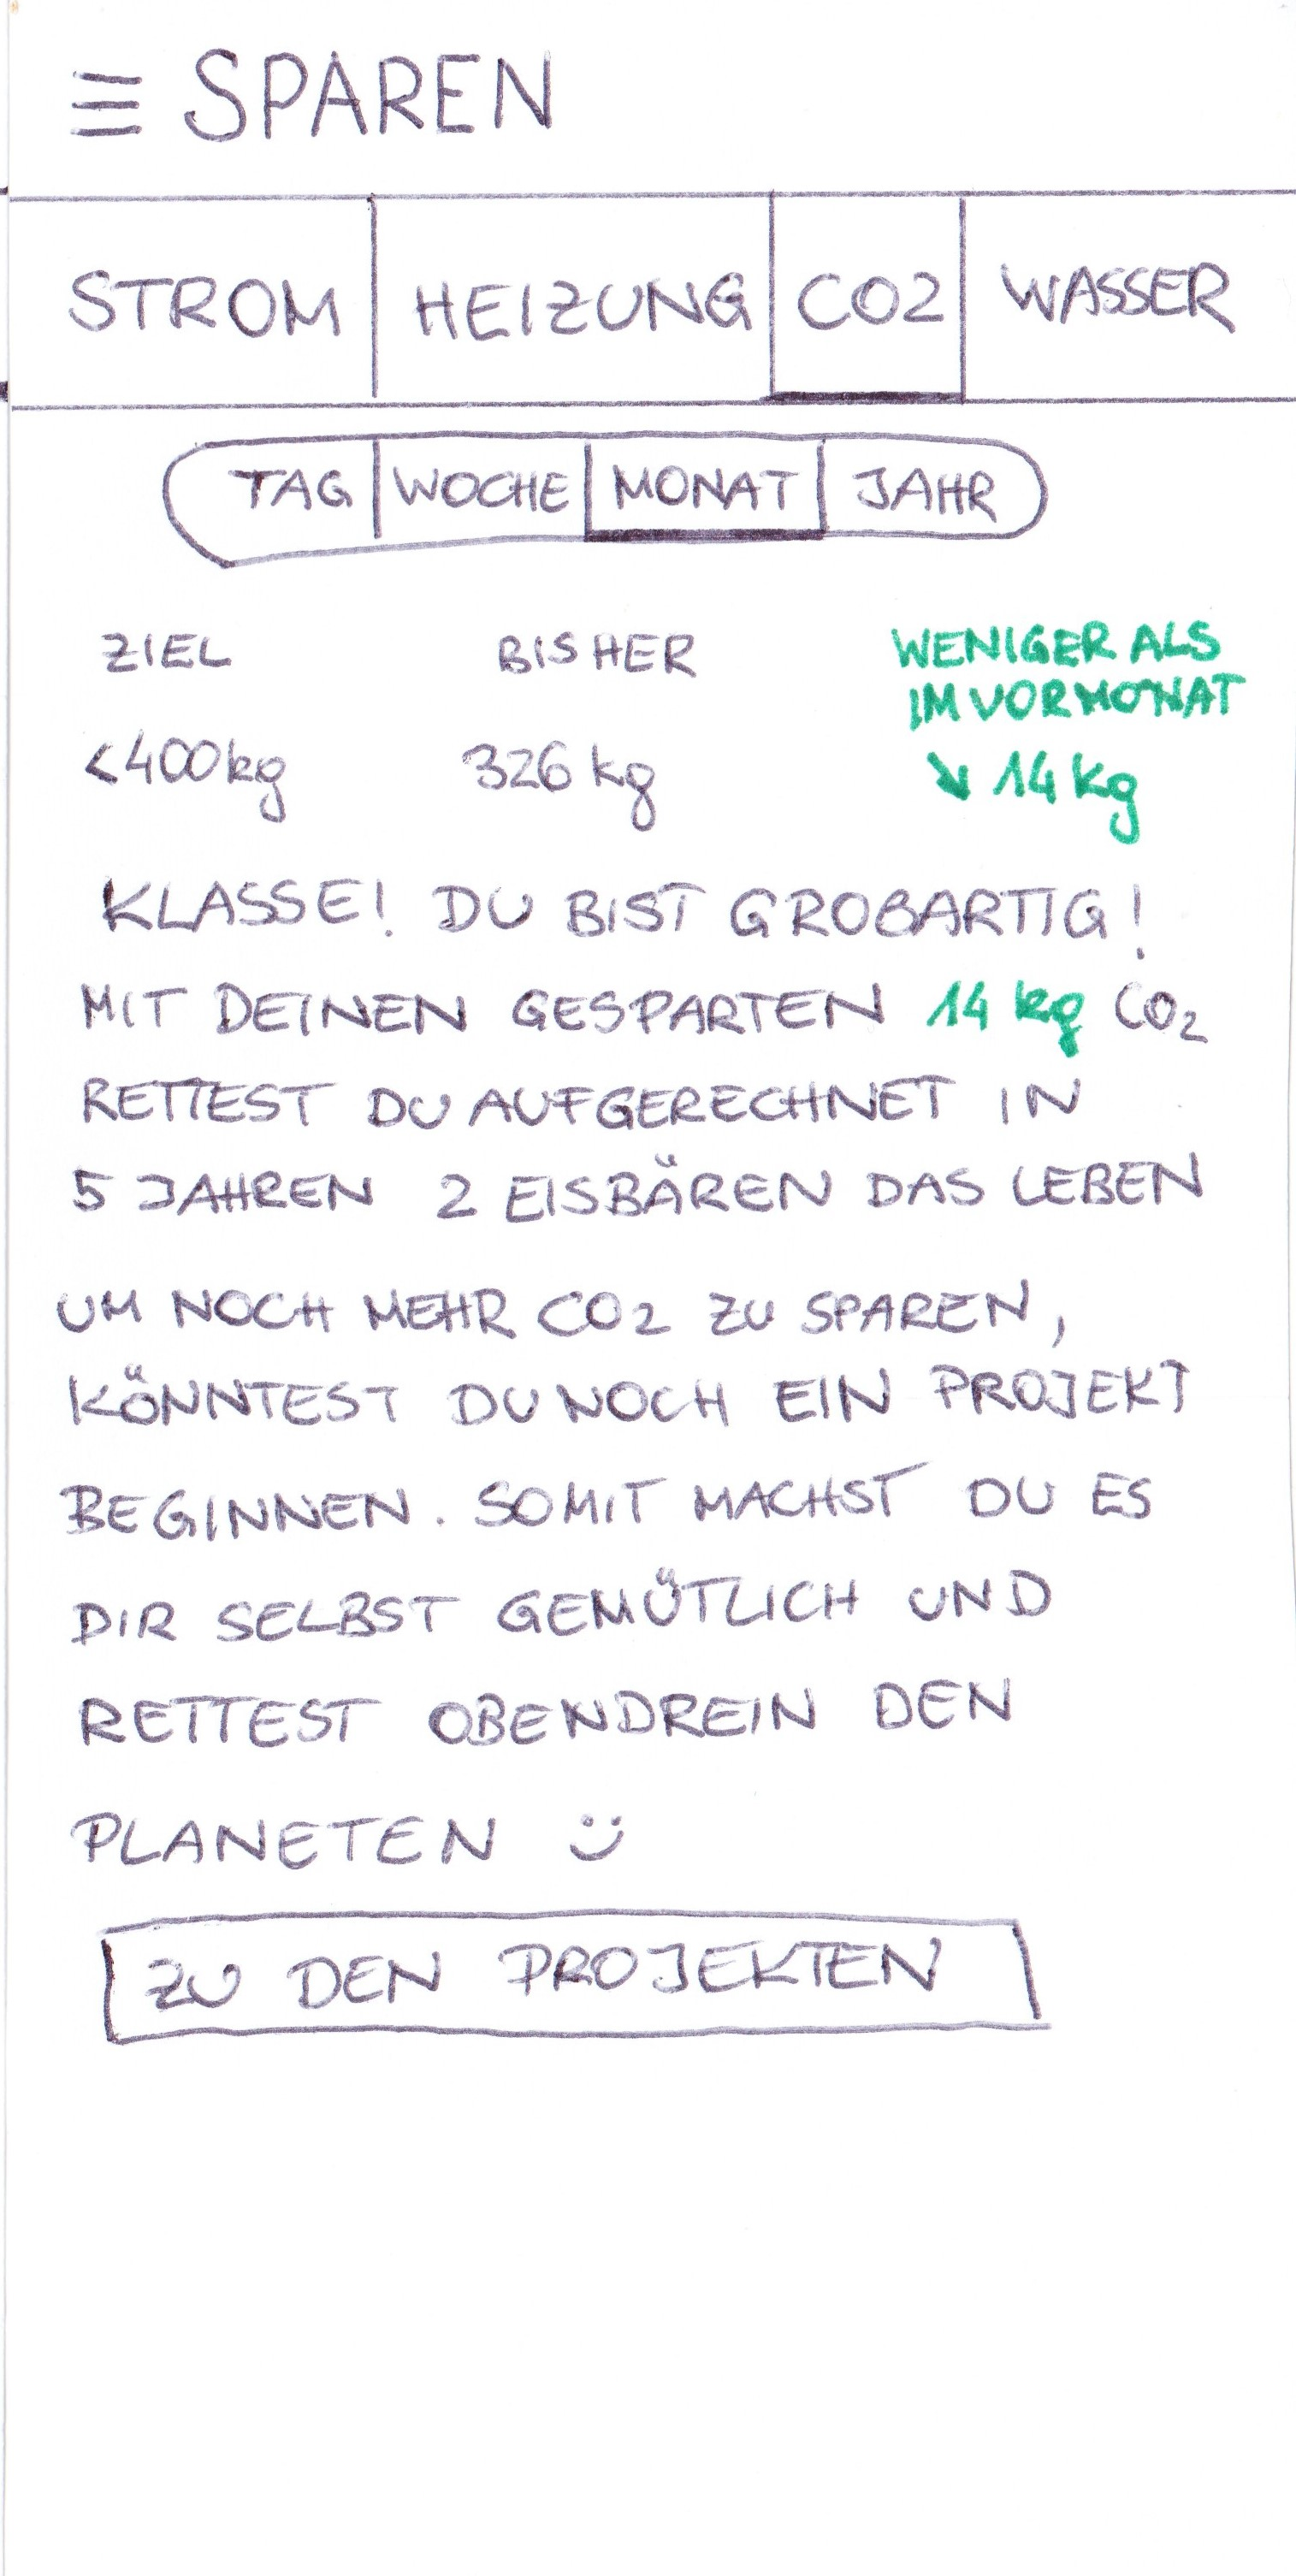
\includegraphics[width=\textwidth]{screens/Sparen_4}
		\subcaption{Hedonist}
		\label{fig:sparen:hedonist}
	\end{subfigure}
	\caption{The paper prototype screens for comparison of savings for all four user segments}
	\label{fig:sparen} % \label has to be placed AFTER \caption (or \subcaption) to produce correct cross-references.
\end{figure}

\subsection*{Guideline 5: Provide the possibility to compare with others for Professionals}

Preparing ones consumption data with other even unknown people is motivating for a Professional.

\textbf{Evidence} \quad The ranking table and the comparison with others is based on the design principles social learning, social comparison, normative influence, competition and recognition, that are described above in the section~\ref{subsubsec:socialsupport}. In the paper prototype sessions the Professionals also liked their proposed screen the most. The following user story was derived from the statement of the Professional test users: \begin{itemize}
	\item As a Professional I want to compare my consumption data with others.
\end{itemize}

\section{Energy-Saving Tips}

The energy-saving tips are subdivided into categories which can be scrolled horizontally as shown in Figure~\ref{tipps}. The interface is the same for all user types but the tips are tailored to the specific preferences. A Hedonist does not get tips that limit comfort, see Figure~\ref{fig:tipps:hedonist}. An Optimizer should not get tips that are written in technical language. A Professional prefers deeper information about a tip and why the appliance of a special behaviour saves money. For Hedonists tips for saving energy or CO2 should not concern longer usage of laptops or entertainment screens, as streaming and use of social media is an important leisure activity for them.

\textbf{Improvements} \quad The projects are more logical to be an extra menu item and not a part of the energy-saving tips. The list of tips can be updated from time to time to make it more interesting.

\begin{figure}[h]
	\centering
	\begin{subfigure}[b]{0.24\columnwidth}
		\centering
		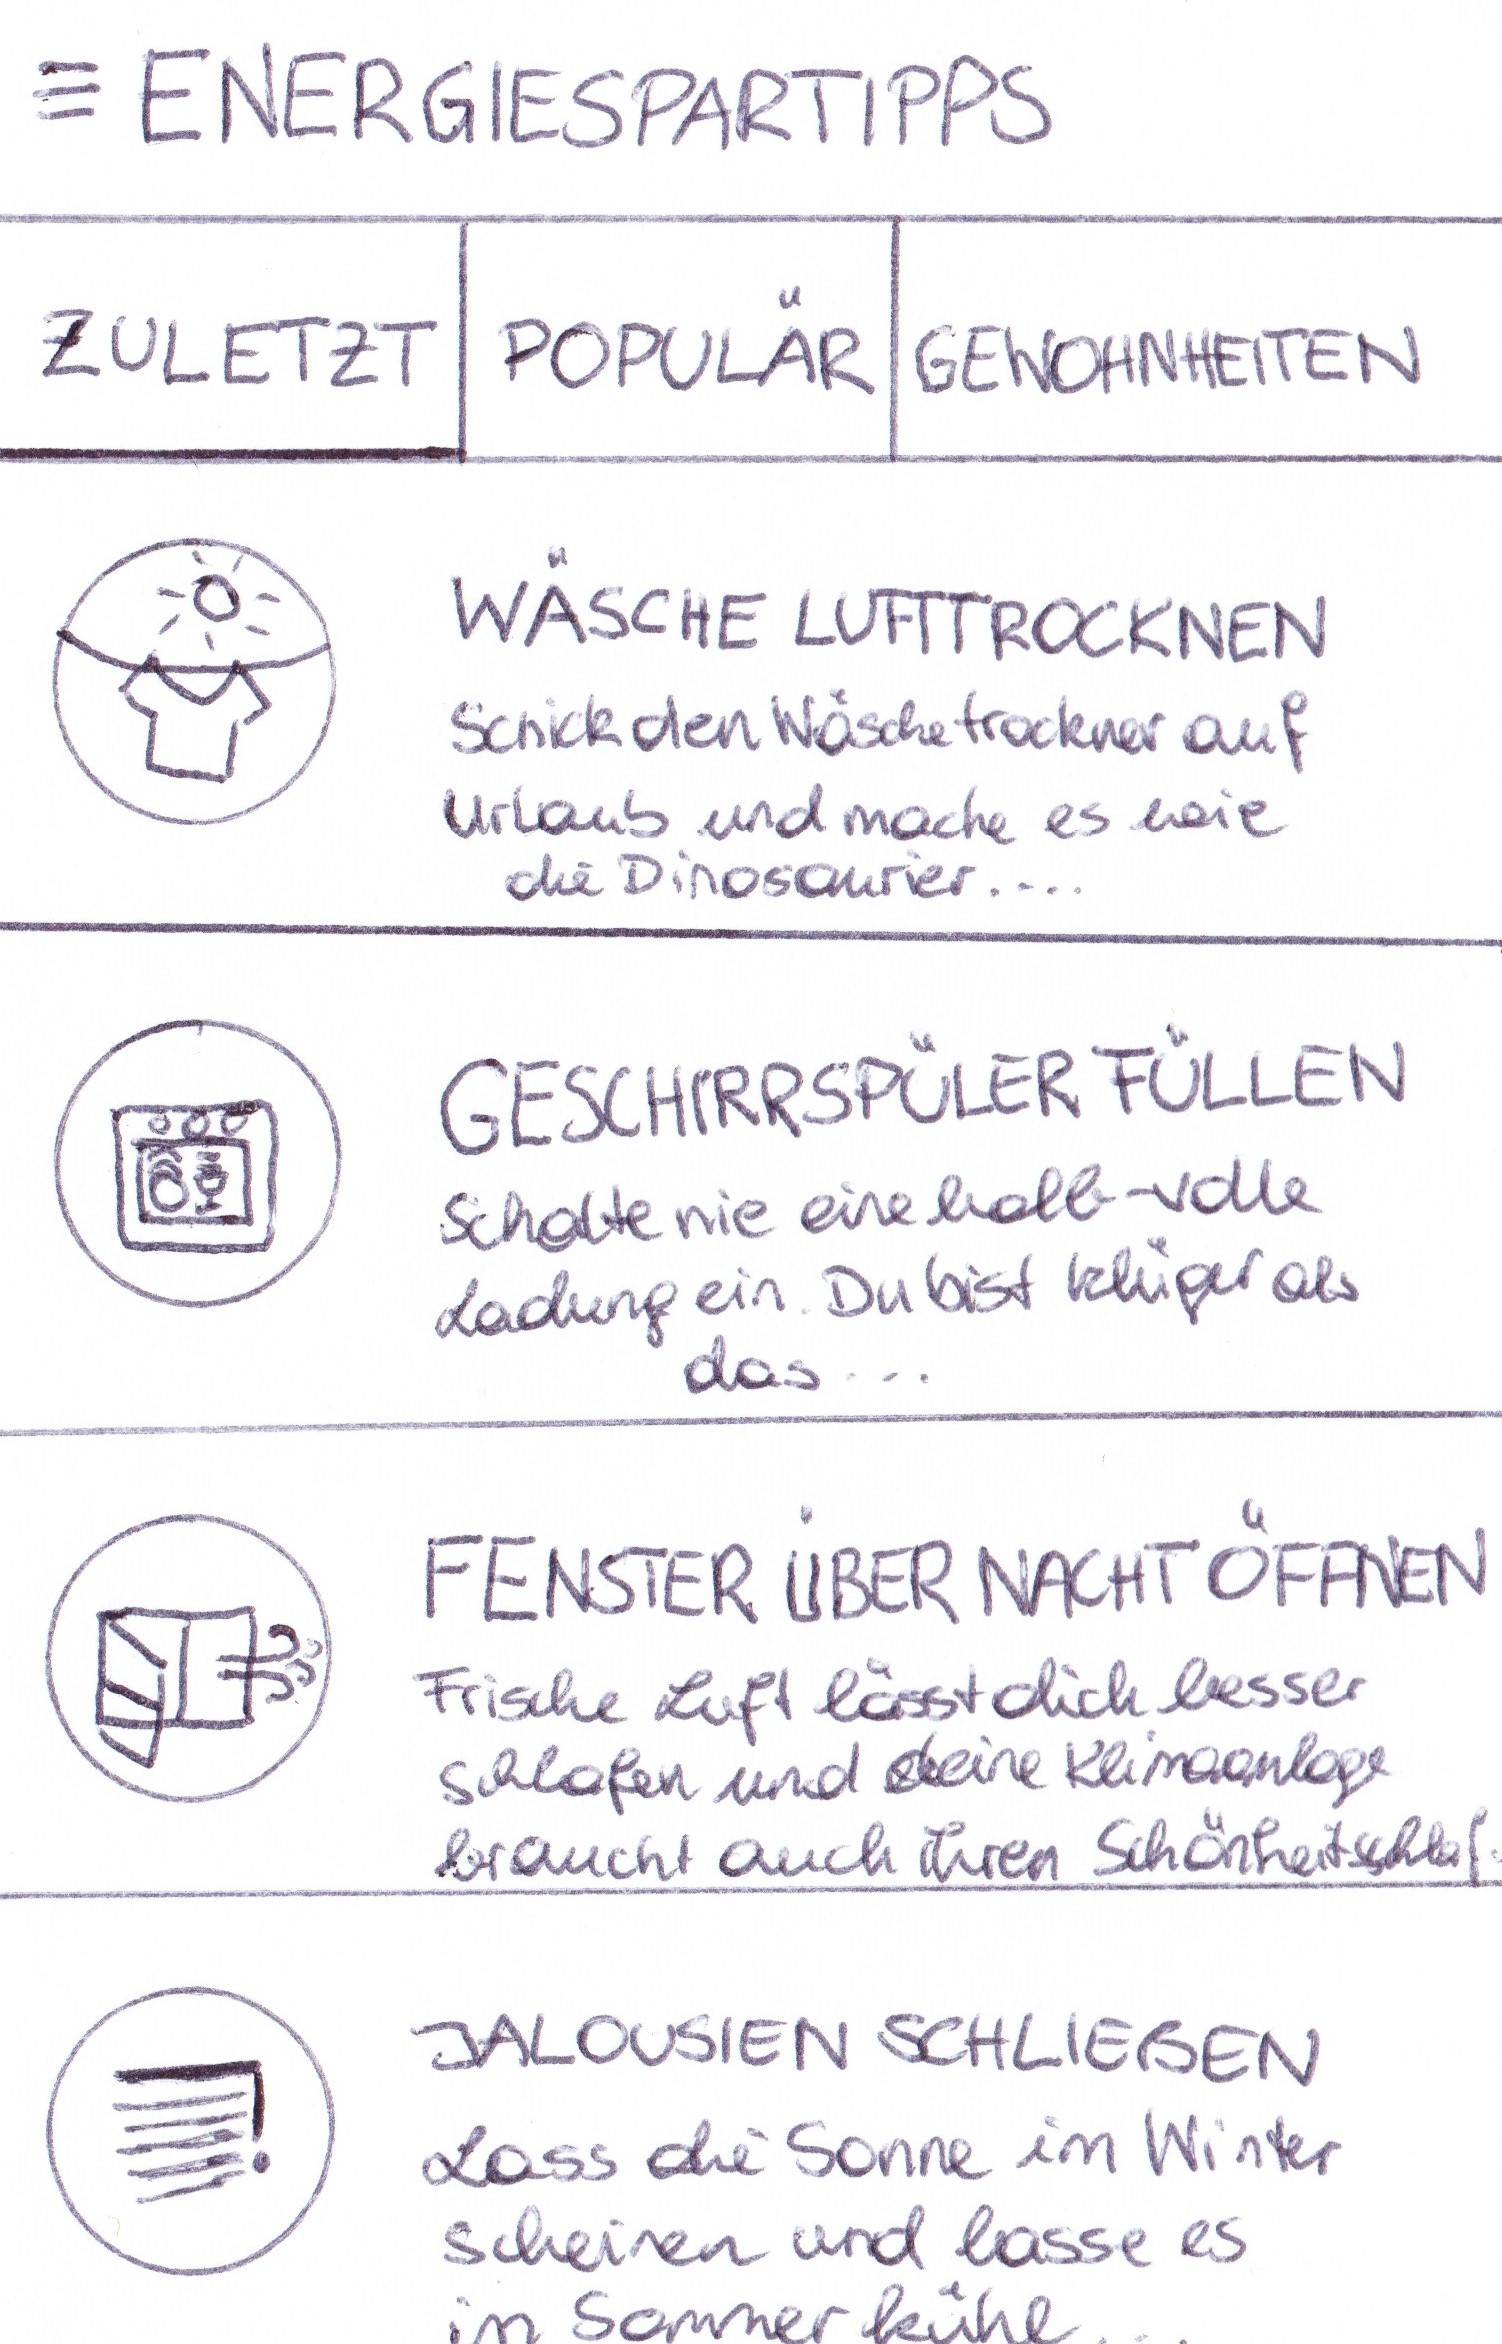
\includegraphics[width=\textwidth]{screens/tipp_1}
		\subcaption{Professional}
		\label{fig:tipps:professional}
	\end{subfigure}
	\begin{subfigure}[b]{0.24\columnwidth}
		\centering
		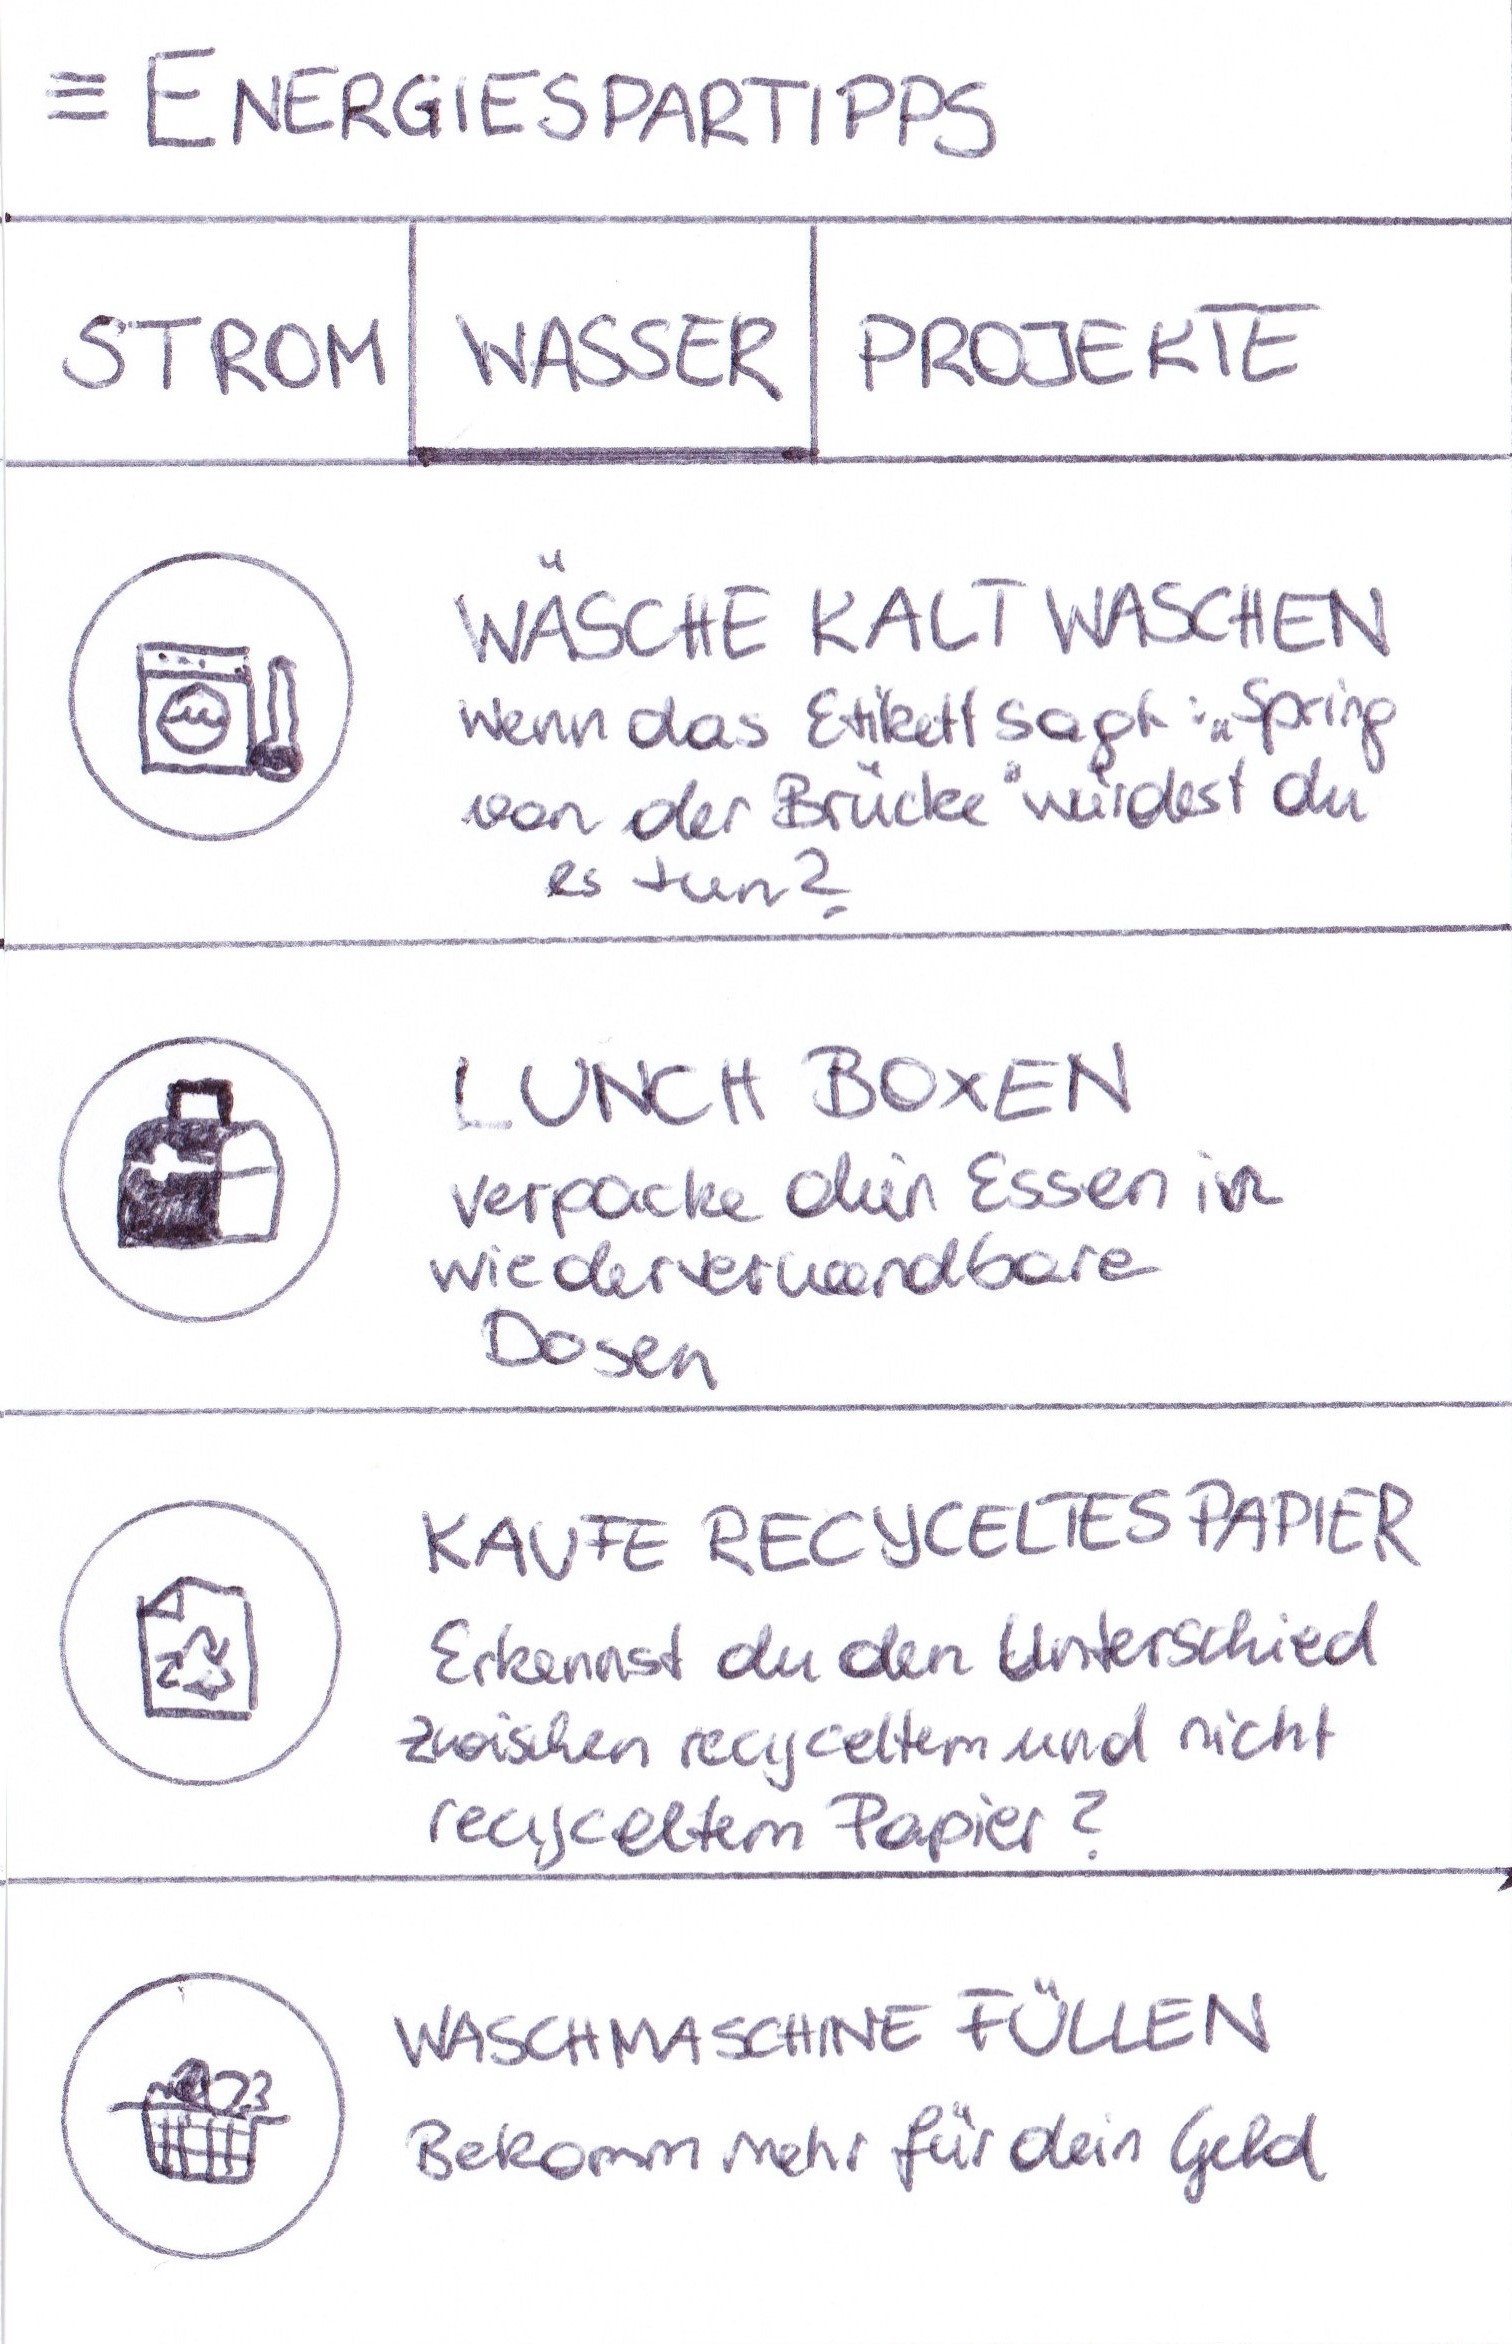
\includegraphics[width=\textwidth]{screens/tipp_2}
		\subcaption{Optimizer}
		\label{fig:tipps:optimizer}
	\end{subfigure}
	\begin{subfigure}[b]{0.24\columnwidth}
		\centering
		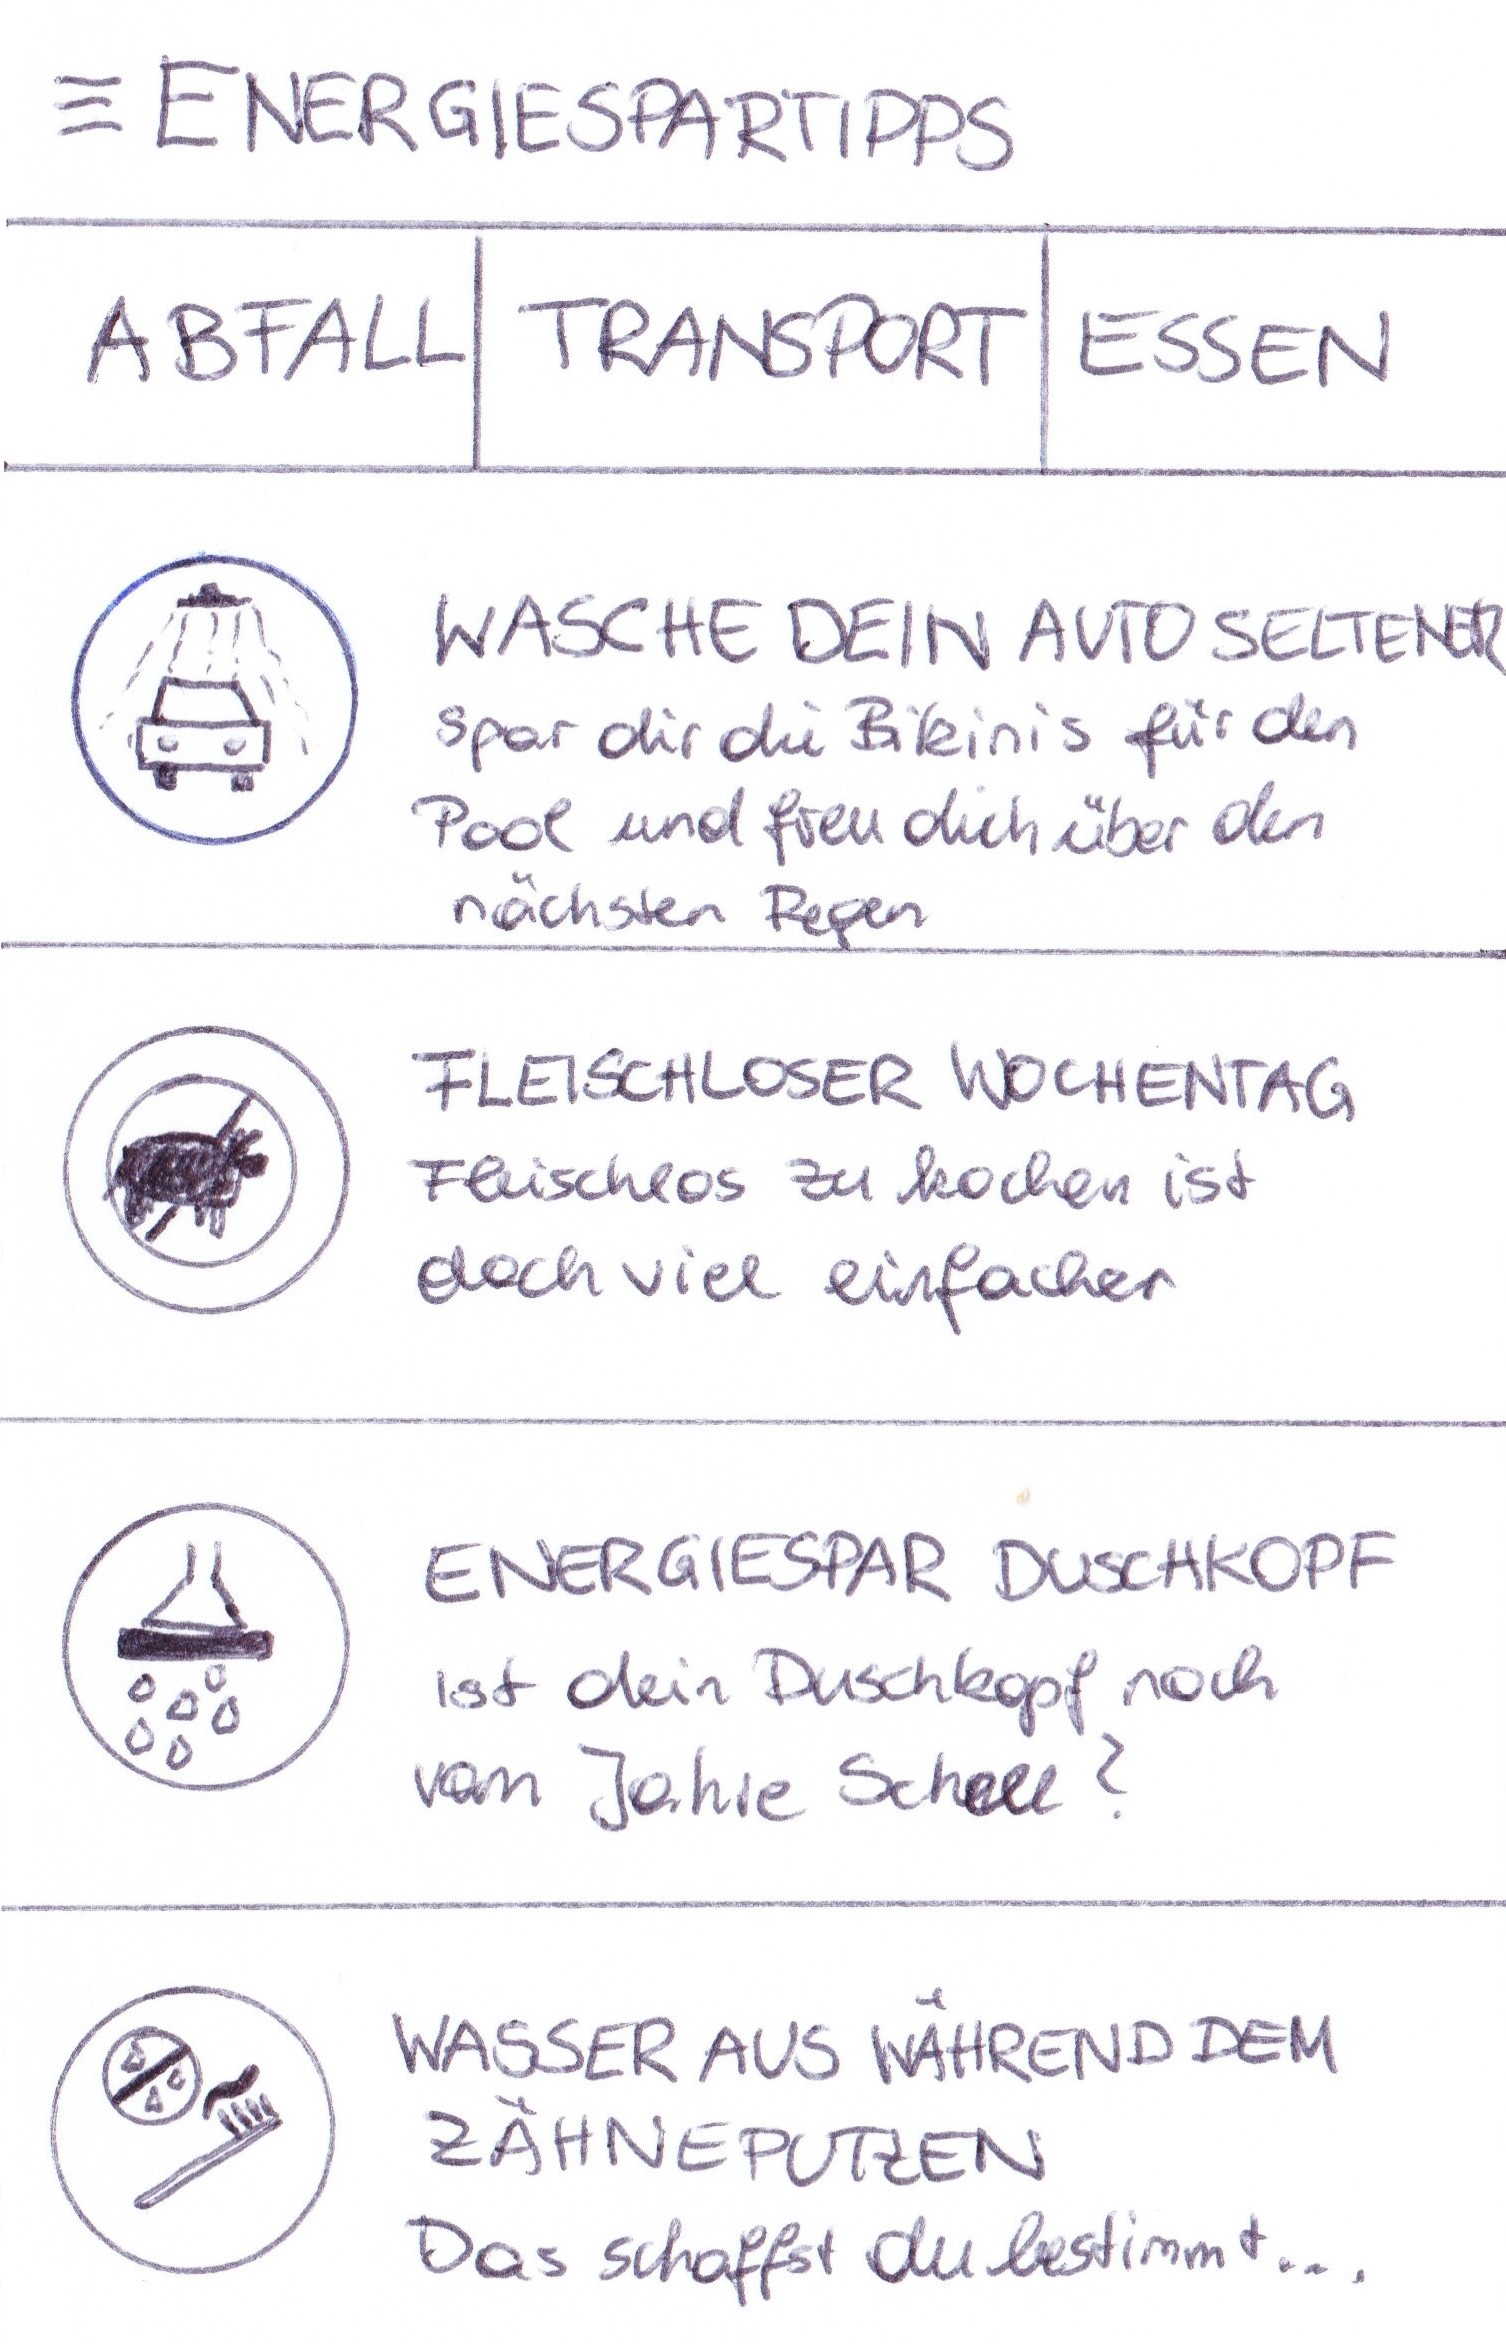
\includegraphics[width=\textwidth]{screens/tipp_3}
		\subcaption{Indifferent}
		\label{fig:tipps:indifferent}
	\end{subfigure}
	\begin{subfigure}[b]{0.24\columnwidth}
		\centering
		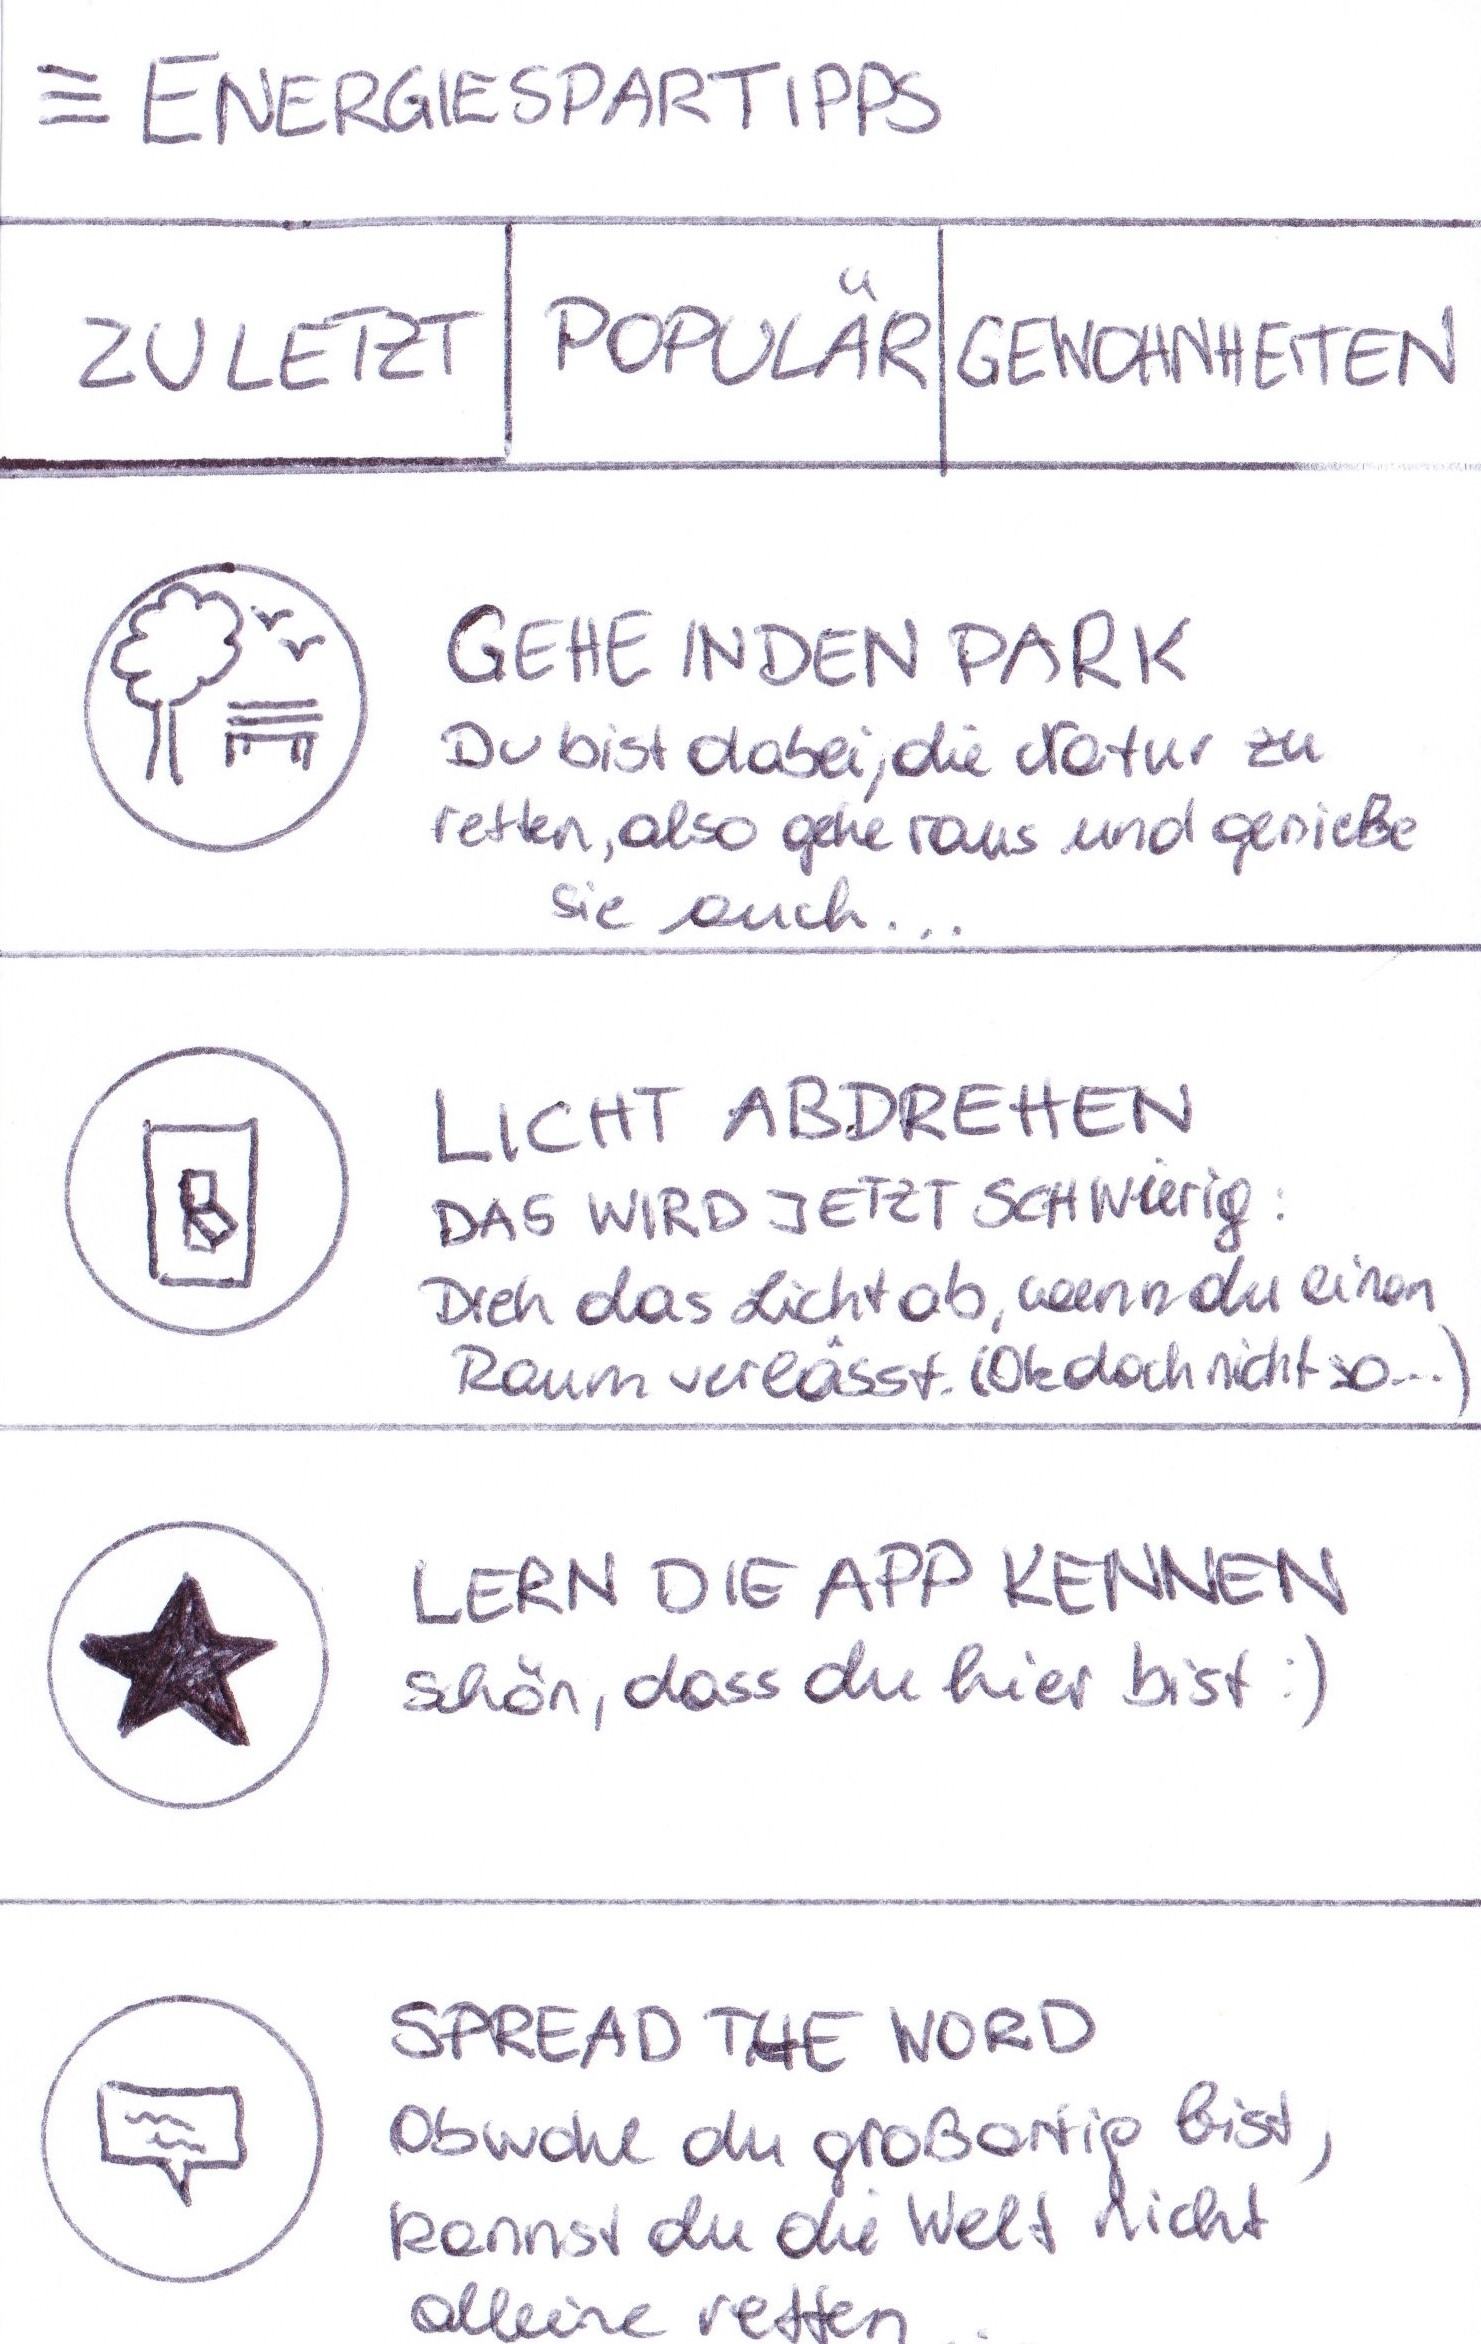
\includegraphics[width=\textwidth]{screens/tipp_4}
		\subcaption{Hedonist}
		\label{fig:tipps:hedonist}
	\end{subfigure}
	\caption{The paper prototype screen for energy saving tips}
	\label{fig:tipps} % \label has to be placed AFTER \caption (or \subcaption) to produce correct cross-references.
\end{figure}

\subsection*{Guideline 6: Avoid to present comfort limiting energy-saving tips to Hedonists}

Hedonists prefer to do projects that save energy for them in the long run and are comfort-oriented. The hedonistic lifestyle with its strong convenience and comfort orientation is in the foreground. In order not to loose them, do not present energy saving tips to Hedonists when they limit comfort.

\textbf{Evidence} \quad As mentioned in the user segmentation section~\ref{chap:usersegmentation} Hedonists do not want to be limited in comfort, which the Hedonist test users confirmed in the paper prototype session. The following user story was derived:

\begin{itemize}
	\item As a hedonist I do not want energy-saving tips that limit my comfort.
\end{itemize}

\subsection*{Guideline 7: Provide deeper information for an energy-saving tip for Professionals}

Professionals are interested in deeper information for saving tips and want to understand how and why a tip works.

\textbf{Evidence} \quad Based on the findings from the study from SCDA, as mentioned in the User Segmentation Section ~\ref{chap:usersegmentation}, Professionals like to dive deeper into the topic. Again the Tailoring design principle is here applied as the other user segments get shorter information to energy-saving tips. The user story for this guideline is:

\begin{itemize}
	\item As a Professional I want to have deeper information for energy-saving tips.
\end{itemize}


\subsection*{Guideline 8: Avoid to motivate a Professional with gamification elements}

Professionals are intrinsically motivated for energy topics and don't need to be sensitized for these topics.

\textbf{Evidence} \quad The professional test user stated that they would not change their behaviour in order to collect trophies. The proceeding in the game does not motivate them to deal with energy topics more deeply. Some said, that it may be interesting to have a look on but the gamification approach is not persuasive for them. 

\subsection*{Guideline 9: Provide optimizers with the information of how much can be saved when following an energy-saving tip}

Optimizer also like to know the concrete benefits of a certain behaviour change. The explanations shall be as close to reality as possible and technical language shall be avoided. The energy feedback is reduced to essential information. The saved costs after a behaviour change shall be visible to provide some kind of reward for the new habits.

\textbf{Evidence} \quad The design principle "Simulation" as described in ~\ref{subsec:primaryTask} is the basis for this guideline. The information of how much can be saved is the link between the cause and effect with regard to the user's behaviour. The test user of the Optimizer workshop session also mentioned that they like to the amount of money that can be saved by following a special tip.

\subsection*{Guideline 10: Reward an Indifferent with game progress for applying a target behaviour}

Indifferents want to be rewarded with game progress for applying a target behaviour. The main goal that we had with Indifferents was to sensitize them for the project. This was best possible with a gamification approach that is an additional motivation for other user segments but the main one for Indifferents.

\textbf{Evidence} \quad The design principle "Reward" of the dialogue support  ~\ref{subsec:dialogueSupport} proposes to reward a target behaviour. The best reward for Indifferents to change behaviour is game progress, which was also found out in the paper prototyping sessions with Indifferents.


\section{Gamification approach}

Gamification is the application of game theory concepts and techniques to activities that normally don't contain gaming elements. The Gamification elements shall help attract consumers to more efficient energy management. The elements proposed by this thesis are trophies, as shown in Figure~\ref{fig:trophaen}. For earning a trophy a special behaviour has to be done. To increase in levels a special amount of trophies need to be saved.

\textbf{Improvements} \quad An improvement that was mentioned from an Indifferent was to not bind trophies to specific labels but to advance in levels when a special amount of trophies is earned, regardless which trophies. This avoids disappointment when a behaviour was done the whole time but the trophy for it could not be earned because the level was not reached.

\begin{figure}[h]
	\centering
	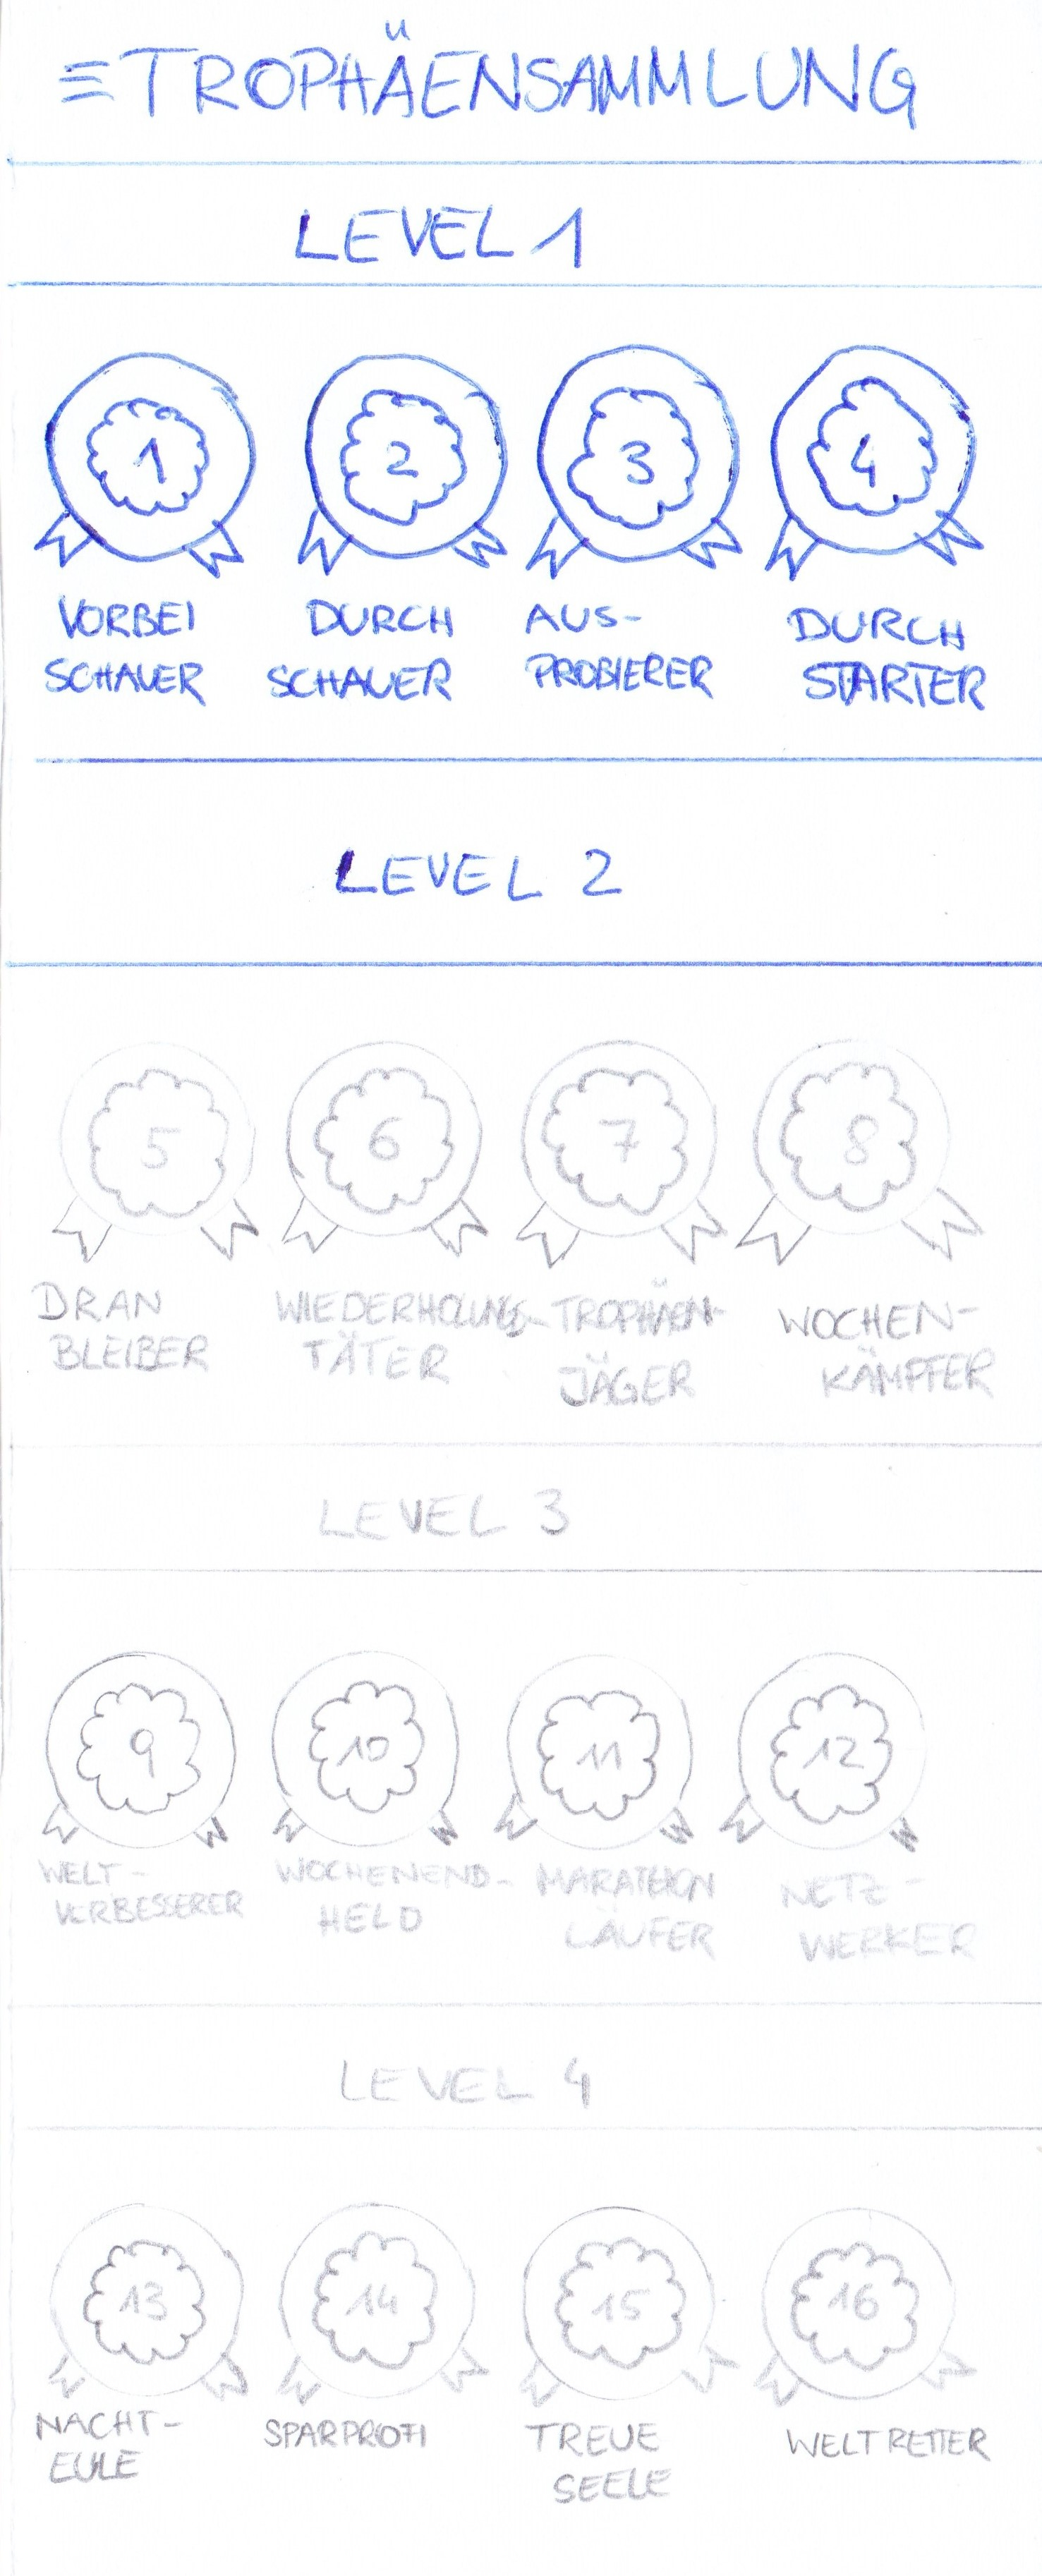
\includegraphics[width=0.24\columnwidth]{screens/Trophaensammlung}
	\caption{Sketch of collection of trophies}
	\label{fig:trophaen} % \label has to be placed AFTER \caption (or \subcaption) to produce correct cross-references.
\end{figure}

\subsection*{Guideline 11: Use gamification elements to sensitize Indifferents to energy-topics}

The Indifferents have low interest in energy topics in general, so the main requirement of the application for this type of user is in the first run to sensitize them for the topic, to raise awareness and to make electricity and CO2 saving appealing to them. To awaken their interest for energy and sustainability a gamification approach is recommended. When the game also has an addictive quality it may be even more beneficial for sensitization.

\textbf{Evidence} \quad The Indifferent in the user prototype session said "...I am the perfect type for this kind of gamification...". The following user story can be derived from this:

\begin{itemize}
	\item As a Hedonist I want to be rewarded with game progress for applying a target behaviour.
\end{itemize} 

\section{Trouble Shooting}
A suggestion how an FAQ screen can look like is shown in Figure~\ref{fig:trouble}. The Professionals and Indifferents like the possibility to read frequently asked questions first, the Optimizer prefer to call first and the Hedonists also like to read but when the solution can not be found in short time they also like to call.

\textbf{Improvements} \quad A chat was proposed by a Professional. In contrast, another Professional would not like a chat. Having the possibility to send an E-mail was categorized as low priority. The telephone number should be at first like in Figure~\ref{fig:trouble} for Optimizer but for the other types, the questions are preferably on the first position.

\begin{figure}[h]
	\centering
	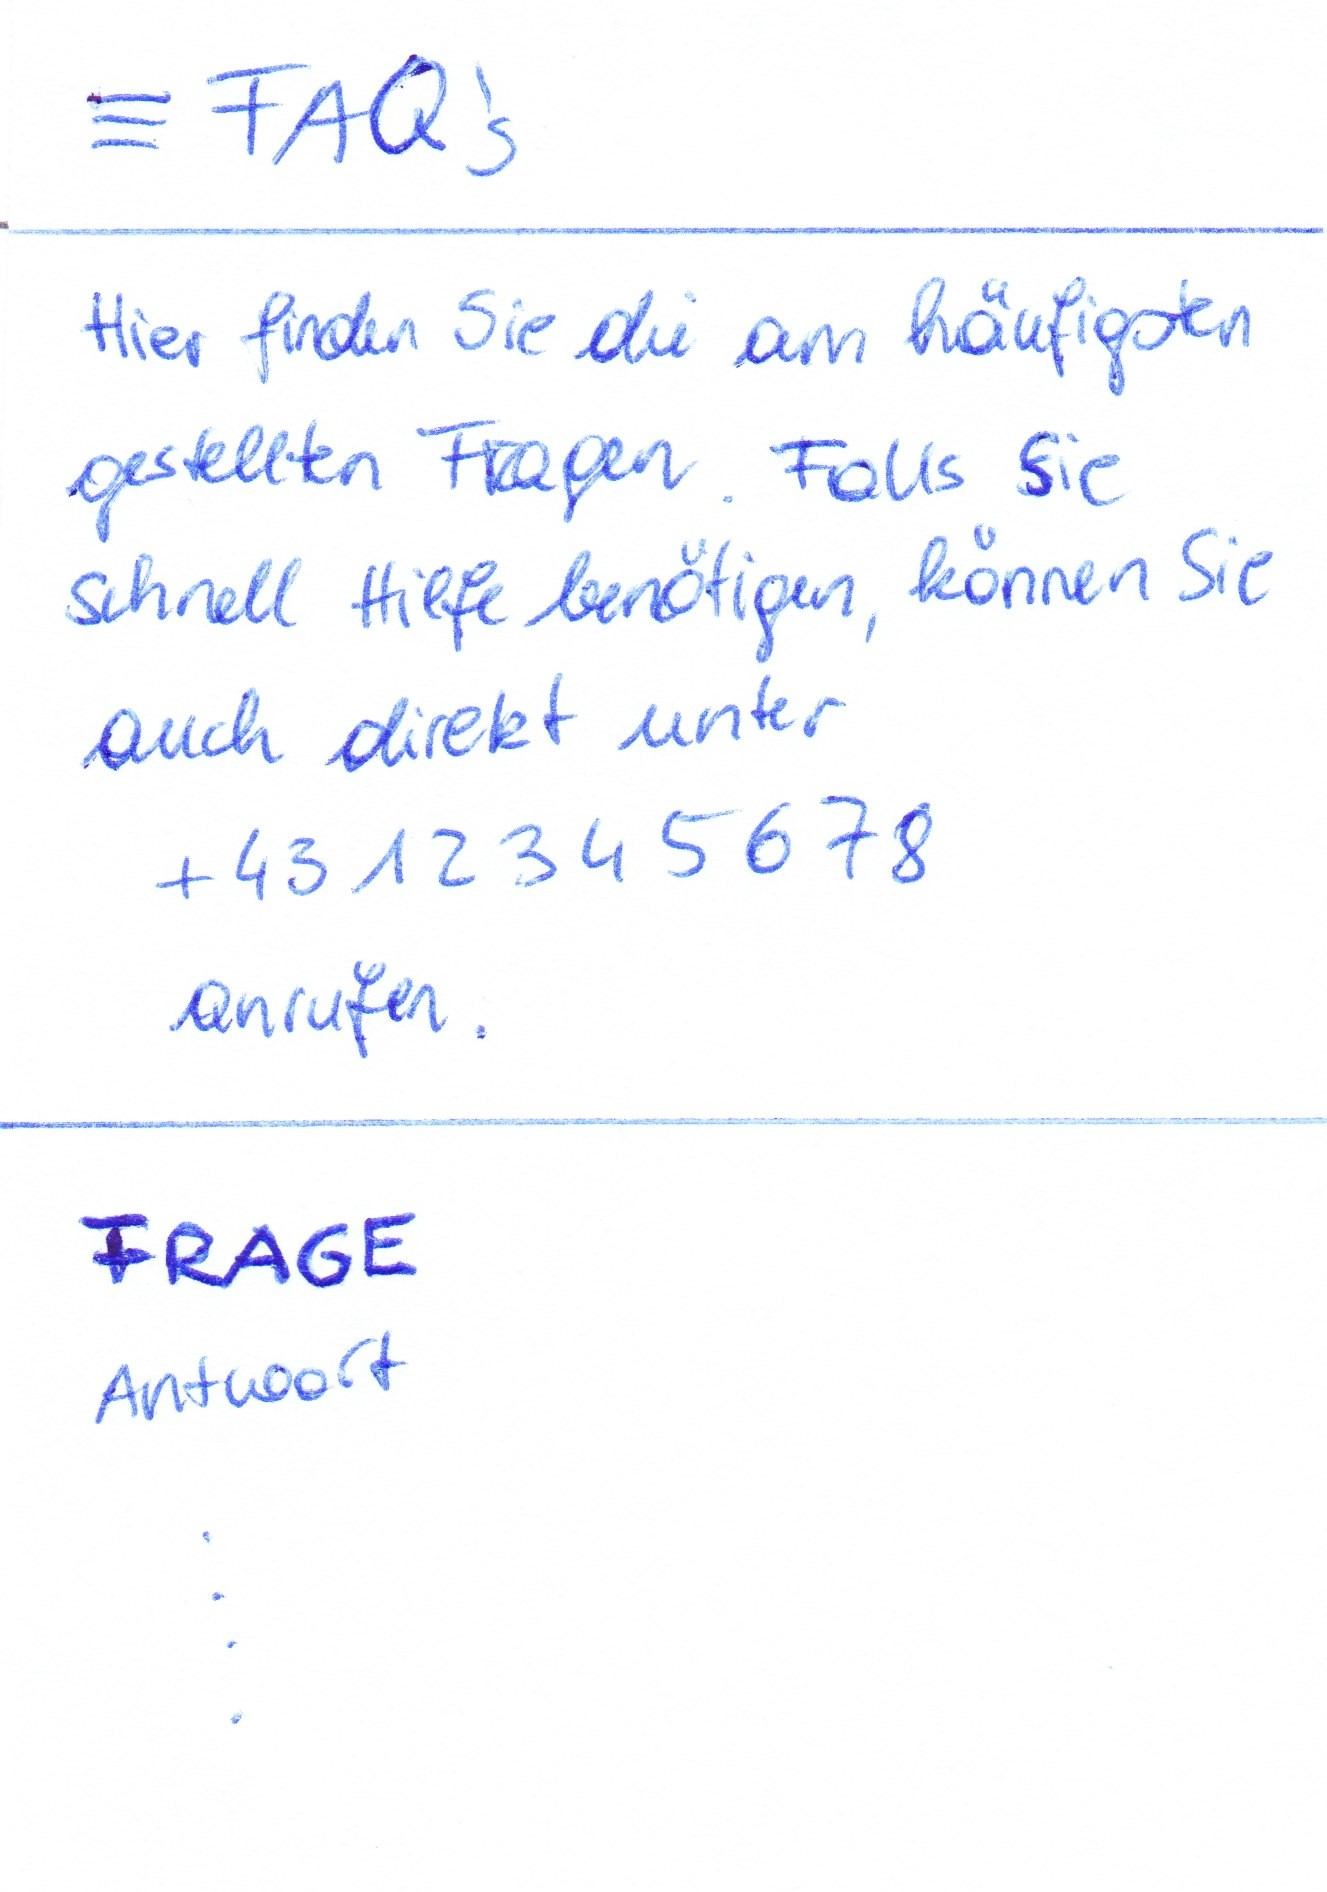
\includegraphics[width=0.24\columnwidth]{screens/FAQs}
	\caption{The proposed screens for Trouble shooting}
	\label{fig:trouble} % \label has to be placed AFTER \caption (or \subcaption) to produce correct cross-references.
\end{figure}

\subsection*{Guideline 12: Provide a hotline for trouble shooting for Optimizer and Hedonists}
For Optimizer trouble shooting shall be easily accessible, in order to reduce the time they are spending with the application and not to loose them on the way.

\textbf{Evidence} \quad In the paper prototyping session with the Optimizer it was wished for an hotline to call immediately when an error occurs. The Hedonist also stated, that calling is preferred to reading the FAQs.


\subsection*{Guideline 13: Provide FAQs for Professionals and Indifferents}

Professionals and Indifferents take the time to read frequently asked questions when a problem occurs. 

\textbf{Evidence} \quad One Professional stated he would read the FAQs carefully before calling the hotline. The Indifferent said, calling was not preferred at all, reading the FAQs or writing a mail would be done before calling.

\section{Communication}

Any interactive system provides some system feedback to the users, mostly via verbal information. The dialogue between computer and human shall help users to keep moving towards their goal or target behaviour.

\subsection*{Guideline 14: Use praise to motivate all energy-users}

Make use of praise via words, images, symbols or even the use of colours as a way to provide user feedback information based on previous behaviour.

\textbf{Evidence} \quad The design principle "Praise", mentioned in \nameref{subsec:dialogueSupport}, applies here. Also the paper prototype sessions showed that praise is the most beneficial way to make users open to persuasion.


\subsection*{Guideline 15: Use concrete instructions and avoid detailed information for Optimizer }

Optimizers prefer less time of interaction and rather like unclear instructions. Notifications and energy-saving tips should give concrete, clear and close to reality handling instructions on how to apply the target behaviour.

\textbf{Evidence} \quad The paper prototyping session with the Optimizer clearly showed that this user segment favours clear handling instructions to reduce the time of applying the wished behaviour. "Reduction", more deeply described in \nameref{subsec:primaryTask}, is the design principle that applies here, as it reduces effort to perform the target behaviour.


\section{Recommendations for improving the ASCR App}

Part of the paper prototype session with the test user was to evaluate the ASCR App on which the prototype was based upon. The Smart Home Control app developed by ASCR and EMAKINA\footnote{https://www.ascr.at/en/ascrs-smart-home-control-app/. Accessed: 02.09.2018} and is available on the Google Play Store\footnote{https://play.google.com/store/apps/details?id=at.ascr.app. Accessed: 02.09.2018}. The app provides an overview of energy consumption, along with all apartment control options. 

Besides that a time-variable electricity tariff has also been implemented with which users can activate households, e.g. running the dishwasher, ironing, charging batteries, etc., at times when electricity is cheaper. The evaluation of the tariff calendar screen revealed a lot of improvements possibilities.


\begin{figure}[h]
	\centering
	\begin{subfigure}[b]{0.3\columnwidth}
		\centering
		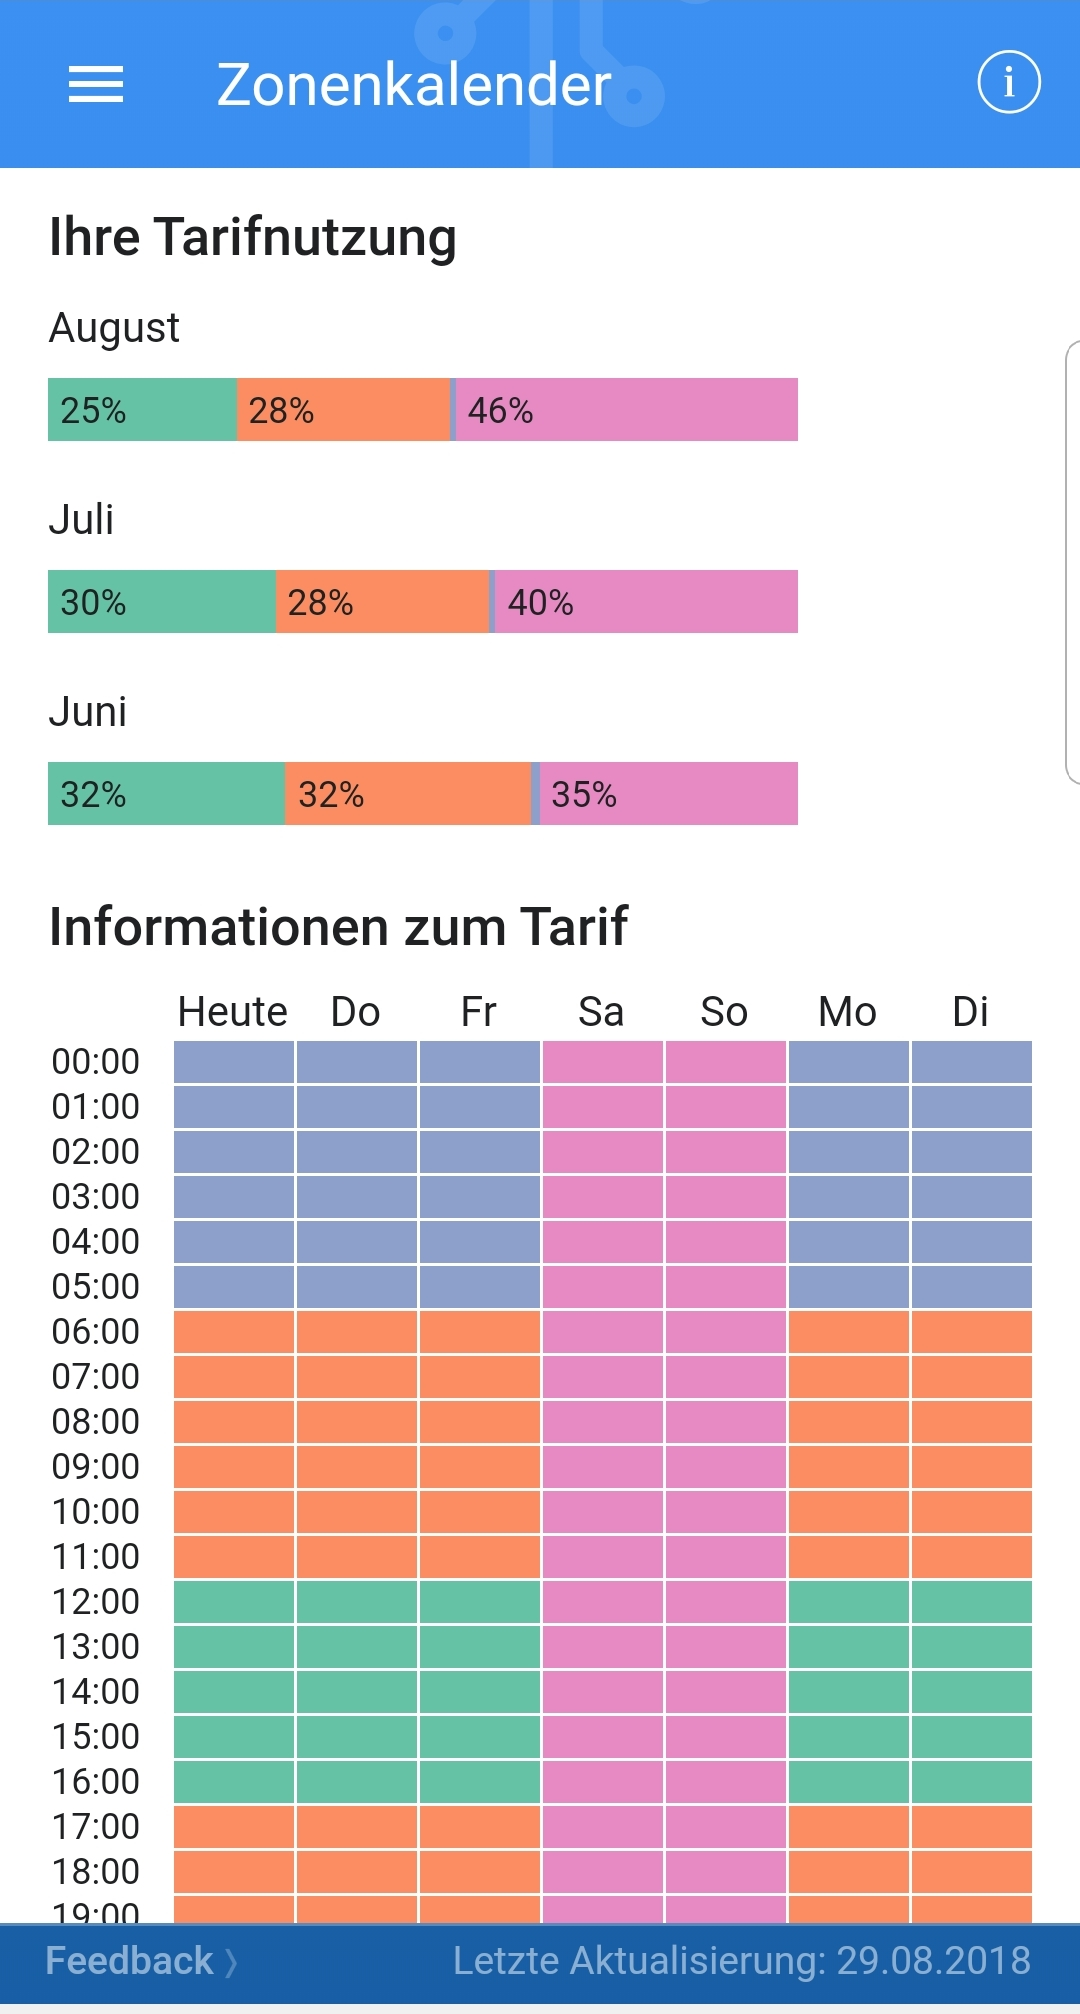
\includegraphics[width=\textwidth]{ascr/zonenkalender1}
		\subcaption{Tariff calendar screen on top}
		\label{fig:zonenkalender1}
	\end{subfigure}
	\begin{subfigure}[b]{0.3\columnwidth}
		\centering
		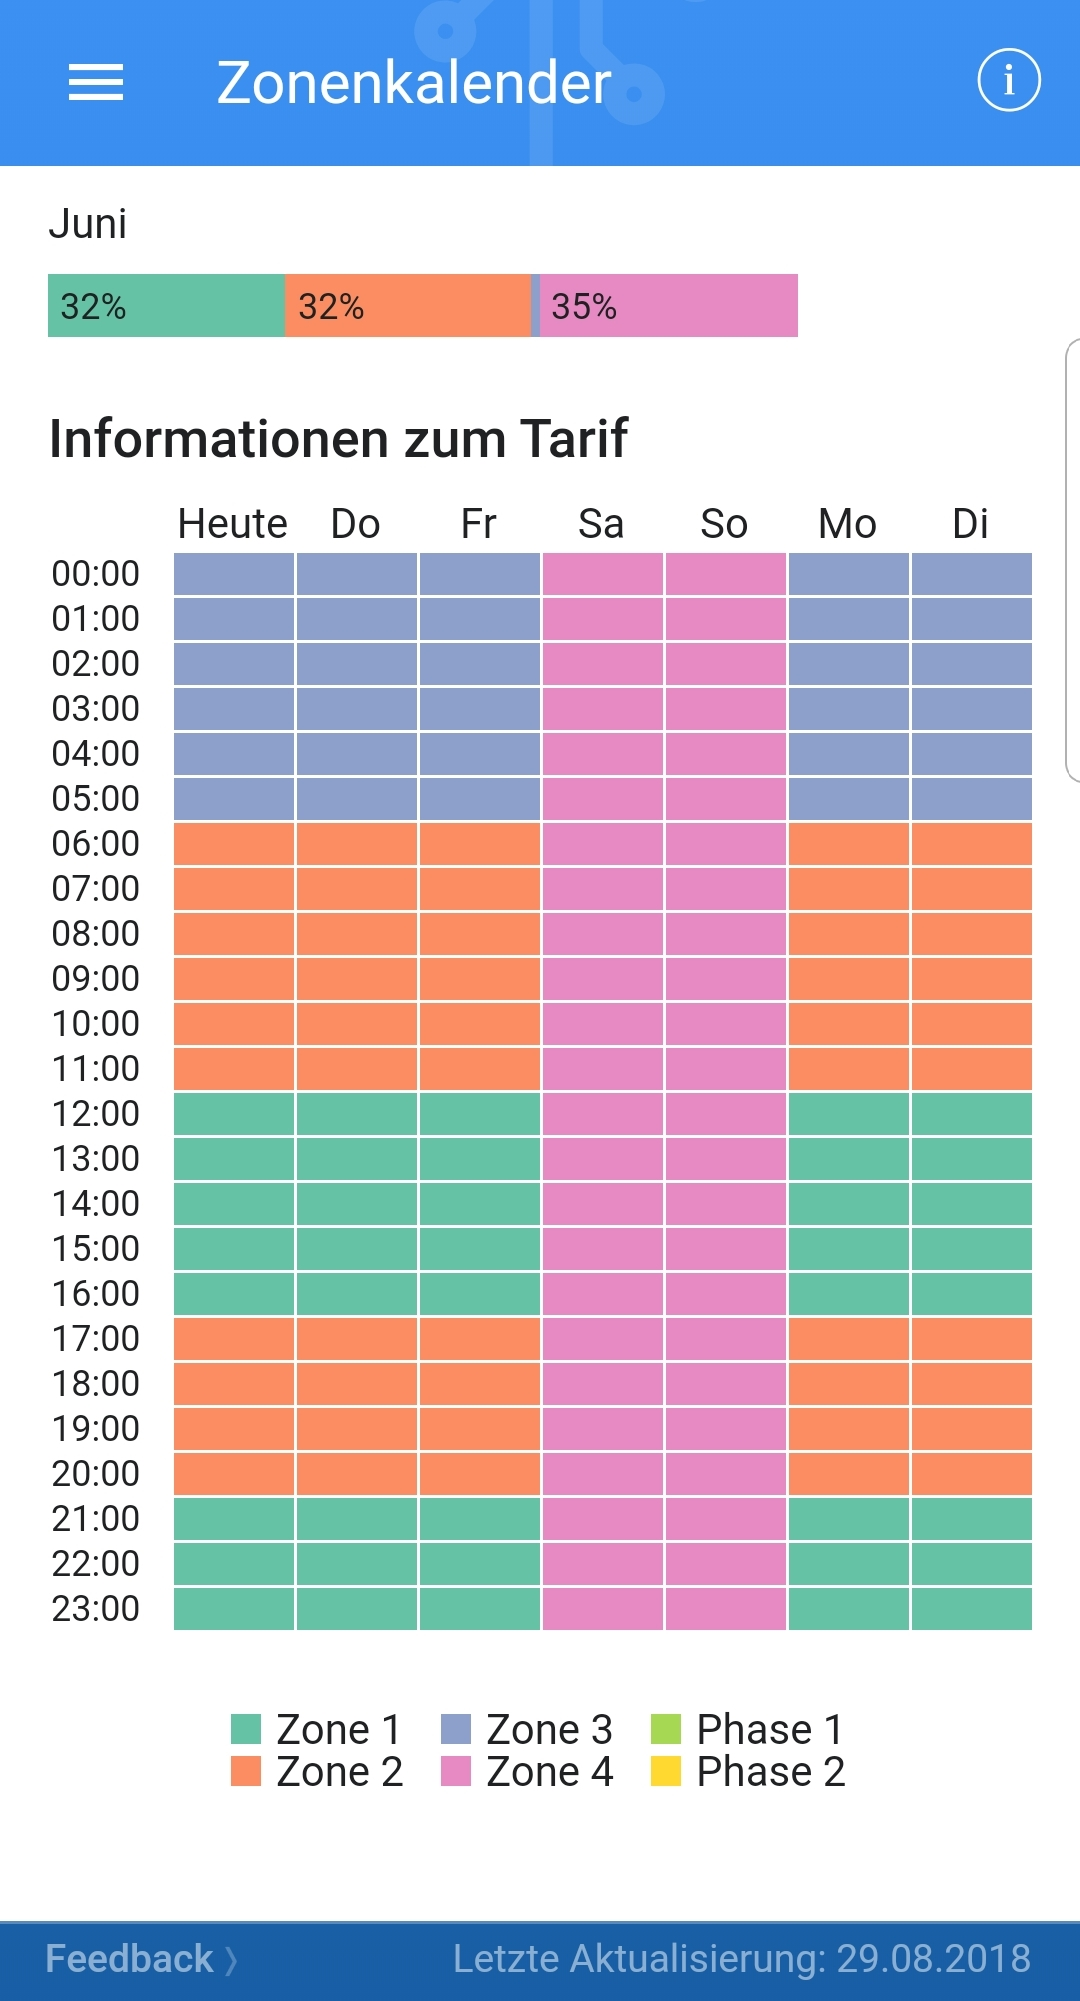
\includegraphics[width=\textwidth]{ascr/zonenkalender2}
		\subcaption{Tariff calendar screen above}
		\label{fig:zonenkalender1}
	\end{subfigure}
	\caption{The screens of the tariff calendar}
	\label{fig:equipmentcontrol} % \label has to be placed AFTER \caption (or \subcaption) to produce correct cross-references.
\end{figure}

\begin{figure}[h]
	\centering
	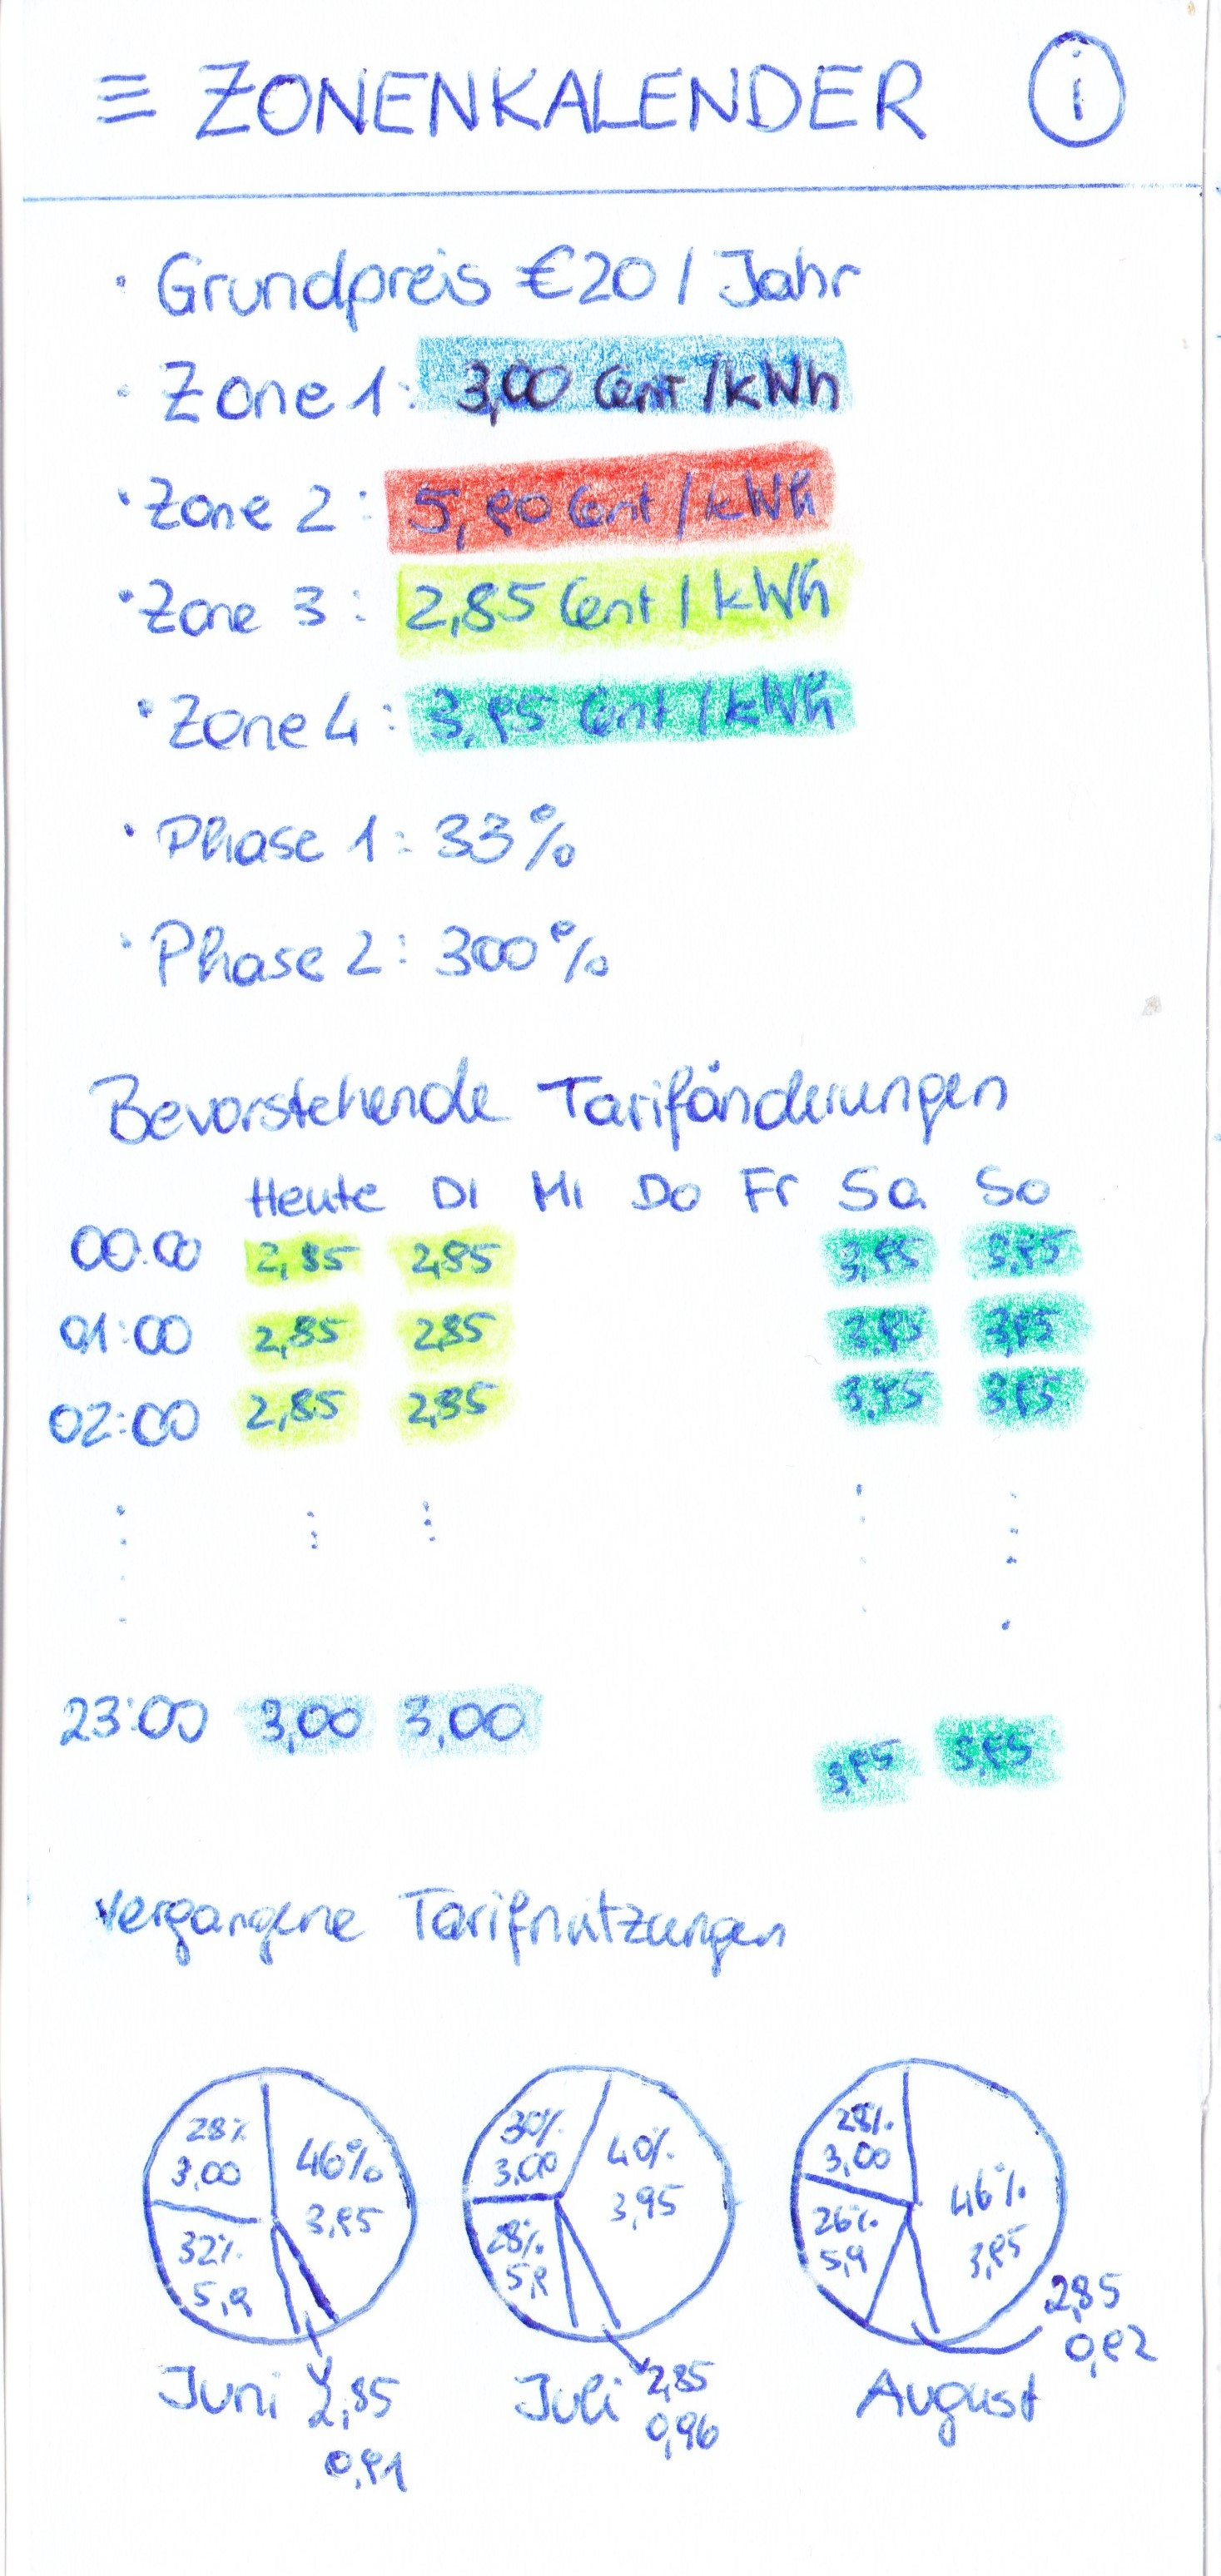
\includegraphics[width=0.3\columnwidth]{screens/Zonenkalender}
	\caption{A recommendation for the tariff description }
	\label{fig:kalender} % \label has to be placed AFTER \caption (or \subcaption) to produce correct cross-references.
\end{figure}

%el be shown in a dashboard, in about how much electricity, water and heating a user consumed, how much carbon-dioxide was produced and how the values can be made better in the sense of reducing consumptions. The screens shall be adapted to the user type to make the information and tips more attractive to a user's interests. The interfaces shall be different for each user but every user should basically have the possibility to do all tasks.
%
%\begin{enumerate}
%	\item As a user I want to have a look on your consumption rate of the last day/week/month/year
%	\item Compare your consumption rate of the last day/week/month/year with the consumption rate of the same week one year earlier.
%	\item Compare your consumption rate of the last week with the average consumption rate of your neighbours
%	\item Find tips on how to save more energy
%	\item Find out what to do to save costs for electricity
%	\item Find out how much you have saved in the last week
%	\item Earn trophies by interacting with the App
%	\item Start a project to install a home automation gadget that saves energy in the long run
%	\item Report a problem
%\end{enumerate}
%In order to elicit the requirements for the graphical user interfaces and to find usability mistakes we make use of Paper Prototyping. 
%
%\subitem{Hedonists}:
%The youngest segment, the Hedonists, are keen on developing technical solutions. The interest in technology can be used to give instructions for programming technical devices and using home automation. The primary motive for the Hedonists is not to save energy but the interest in technology. This will be considered in the notifications and tips of the day. The hedonistic lifestyle with its strong convenience and comfort orientation is in the foreground. For a hedonist the comfort gain is of great relevance. Programming and establishing home automation aspects is a great interface between the aim of saving energy and the affinity of technology.
%
